% !TEX root = main.tex
\section{Method}

\subsection{Programming a BWIM system}
Describe shortly how the BWIM system have been programmed.
Keywords:
\begin{itemize}
\item Beam bridge model
\item Producing a strain history through influence lines
\item Finding the speed of the train
\item Finding Axle distances
\item Solving system for axle weights
\end{itemize}
This master project began by learning how a BWIM-system works, and to then create a working model performing BWIM. To not make this a too big project this meant building a simple beam model of a bridge in Matlab, and simulate moving loads crossing it.

A simple flow diagram describing the intial BWIM program:
\begin{figure}[H]
	\centering
	% 
\tikzset{
  terminal/.style={draw, rounded rectangle, text width=3cm, text centered},
  process/.style={draw, text width=3cm, text centered},
  decision/.style={draw, diamond, aspect=2, text width=3cm, text centered},
  delay/.style={draw, rounded rectangle, rounded rectangle west arc=none, text width=3cm, minimum height=1cm, text centered},
  line/.style={draw, -latex}
}
\begin{tikzpicture}
  \node[terminal] (main) {Main script};
  \node[process, above=1cm of main] (createInfl) {create influence line};
  \node[process, right=2cm of main] (createStrain) {create strain signal};
  \node[process, below=2cm of main] (findSpeed) {find train speed};
  \node[process, left=1cm of findSpeed] (findAxleDist) {find axle distances};
  \node[process, left=2cm of main] (calcAxleWeights) {calculate axle weights};

  \draw[line] (main) -- (createInfl);
  \draw[line] (main) -- (createStrain);
  \draw[line] (main) -- (findSpeed);
  \draw[line] (findSpeed.west) -- (findAxleDist.east);
  \draw[line] (main) -- (calcAxleWeights);
\end{tikzpicture}%

\end{figure}


\subsubsection{Producing a strain signal}
Through the theoretical moment influence lines of the beam, a strain signal can be built through the moment-strain relationship, found in equation\ref{equation:moment_strain}, for a given set of axle weights. A simple beam bridge model, as seen in figure \ref{figure:beam_model}, will not recreate a actual bridge strain signal but will be used to create a working BWIM system. The produced strain signal will differ from an actual strain signal mostly because of dynamics, from the train and bridge, and because actual boundary conditions of a bridge will differ from the boundary conditions of a simple beam model. The strain sensors will also produce noise distorting the signal.

To make as good a signal as possible, some effort were placed into recreating the effect mentioned above. To add noise to the signal, white gaussian noise was included in the signal through Matlabs wgn function "http://se.mathworks.com/help/comm/ref/wgn.html".


This strain signal could then be used as a base to build the code for a BWIM system.

\begin{figure}[htpb]
	\begin{tikzpicture}
		\draw[thick] (0,0) to (5,0);
		\node[ledd fast={0}{0}{0}] (ledd) {};
		\node[ledd skyve={5}{0}{0}] (skyveledd) {};
		%\draw[->] (0,1) to {$\scriptstyle g$} (0,.1);
		\node (a) at (1,1.5) {};
		\node (b) at (1,.1) {};
		\draw[-open triangle 90] (a) to node[pos=-.4] {$axle 2$} (b);
		\node (c) at (3.5,1.5) {};
		\node (d) at (3.5,.1) {};
		\draw[-open triangle 90] (c) to node[pos=-.4] {$axle 1$} (d);
		\node (e) at (3.5,1) {};
		\node (f) at (4.5,1) {};
		\draw[-open triangle 90] (e) to node[pos=1.2] {$v$} (f);
		\node (g) at (1,.5) {};
		\node (h) at (3.5,.5) {};
		\draw[open triangle 90-open triangle 90] (g) to node[above] {$axle spacing$} (h);
		%\draw (2.5,0) circle [radius=0.1] {sensor};
		%\node[draw,circle] (s) at (2.5,0){};
		\filldraw
		(2.5,0) circle (2pt) node[align=left,   below] {strain sensor};
	\end{tikzpicture}
%\captionof{figure}{Beam model for initial BWIM}
\caption{Beam model for developement}
\label{figure:beam_model}

\end{figure}

\begin{figure}[htpb]
	\begin{tikzpicture}
		\draw[thick] (0,0) to (10,0);
		\node[ledd fast={0}{0}{0}] (ledd) {};
		\node[ledd skyve={10}{0}{0}] (skyveledd) {};
		% \node[spring={3}{0}{0}] (spring) {};
		% \node[spring={6}{0}{0}] (spring) {};
		%\draw[->] (0,1) to {$\scriptstyle g$} (0,.1);
		\node (a) at (1,1.5) {};
		\node (b) at (1,.1) {};
		\draw[-open triangle 90] (a) to node[pos=-.4] {$axle 2$} (b);
		\node (c) at (3.5,1.5) {};
		\node (d) at (3.5,.1) {};
		\draw[-open triangle 90] (c) to node[pos=-.4] {$axle 1$} (d);
		\node (e) at (3.5,1) {};
		\node (f) at (4.5,1) {};
		\draw[-open triangle 90] (e) to node[pos=1.2] {$v$} (f);
		\node (g) at (1,.5) {};
		\node (h) at (3.5,.5) {};
		\draw[open triangle 90-open triangle 90] (g) to node[above] {$axle spacing$} (h);
		%\draw (2.5,0) circle [radius=0.1] {sensor};
		%\node[draw,circle] (s) at (2.5,0){};
		% \node[ledd fast={2}{0}{0}] (ledd) {};
		% \draw (2,-.75) -- (2.25,-1) -- (1.75,-1.25) -- (2.25,-1.5) -- (1.75,-1.75); % spring""
		\node[ledd spring={2}{0}{0}] (skyveledd) {};
		\node[ledd spring={4}{0}{0}] (skyveledd) {};
		\node[ledd spring={6}{0}{0}] (skyveledd) {};
		\node[ledd spring={8}{0}{0}] (skyveledd) {};
		\filldraw
		(2.5,0) circle (2pt) node[align=left,   below] {strain sensor};
	\end{tikzpicture}
%\captionof{figure}{Beam model for initial BWIM}
\caption{A more realistic beam bridge model}
\label{figure:beam_model_alt}

\end{figure}


\subsubsection{Finding the speed of the train}
Two working methods of finding the speed of a passing train were developed:
\begin{itemize}
 \item By identifying peaks in the strain history for two different sensors, representing the same axle. The distance between the two sensors and the time difference between the found peaks should theoretically give a good estimate of the trains velocity.
 \item Through doing cross correlation between two sensors strain history. This involves finding the phase difference, or lag, between the signals. The known distance between the strain gauges should then along with a constant, based on distance between sensors, give a reliable estimate of train velocity. INSERT PLOT OF CORRELATION AND SHOW MATHEMATICAL EQUATION DESCRIBING CROSS CORRELATION.
\end{itemize}

\subsection{Finding influence lines}
Describe how influence lines have been found from the given strain history from Lerelva Bridge.
Keywords:
\begin{itemize}
\item Matrix method
\item Optimization
\item Speed
\end{itemize}
\subsubsection{Matrix method}
Describe the matrix method.

\subsubsection{Optimization}
Describe how optimization can be used to find optimal influence lines for the bridge.

\subsection{System setup}
\label{system_setup}
To test the BWIM-program on actual data, we Gunnstein, Daniel set up a BWIM-system to gather strain data from actual train passings. The subject bridge were Lerelva-Bridge in Trondheim, figure \ref{fig:lerelva_bridge}, a typical Norwegian steel railway bridge. Three strain gauges, \SI{3}{\mm} \SI{120}{ohms} from HBM, were placed by the support towards Trondheim on the first section of the longitudinal stringer, see figure \ref{fig:strain_gauges}. The sensors were placed with \SI{1}{\m} spacing around the middle of the stringer section. These strain gauges were connected to a National Instruments compactDAQ with module NI 9235 which produced an continuous data flow to a standard laptop, see figure \ref{fig:instruments}. A Kipor generator was brought for power.
% INSERT SYSTEM IMAGE HERE
\begin{figure}[H]
	\centering
	\begin{subfigure}[t]{0.49\textwidth}
    \centering
    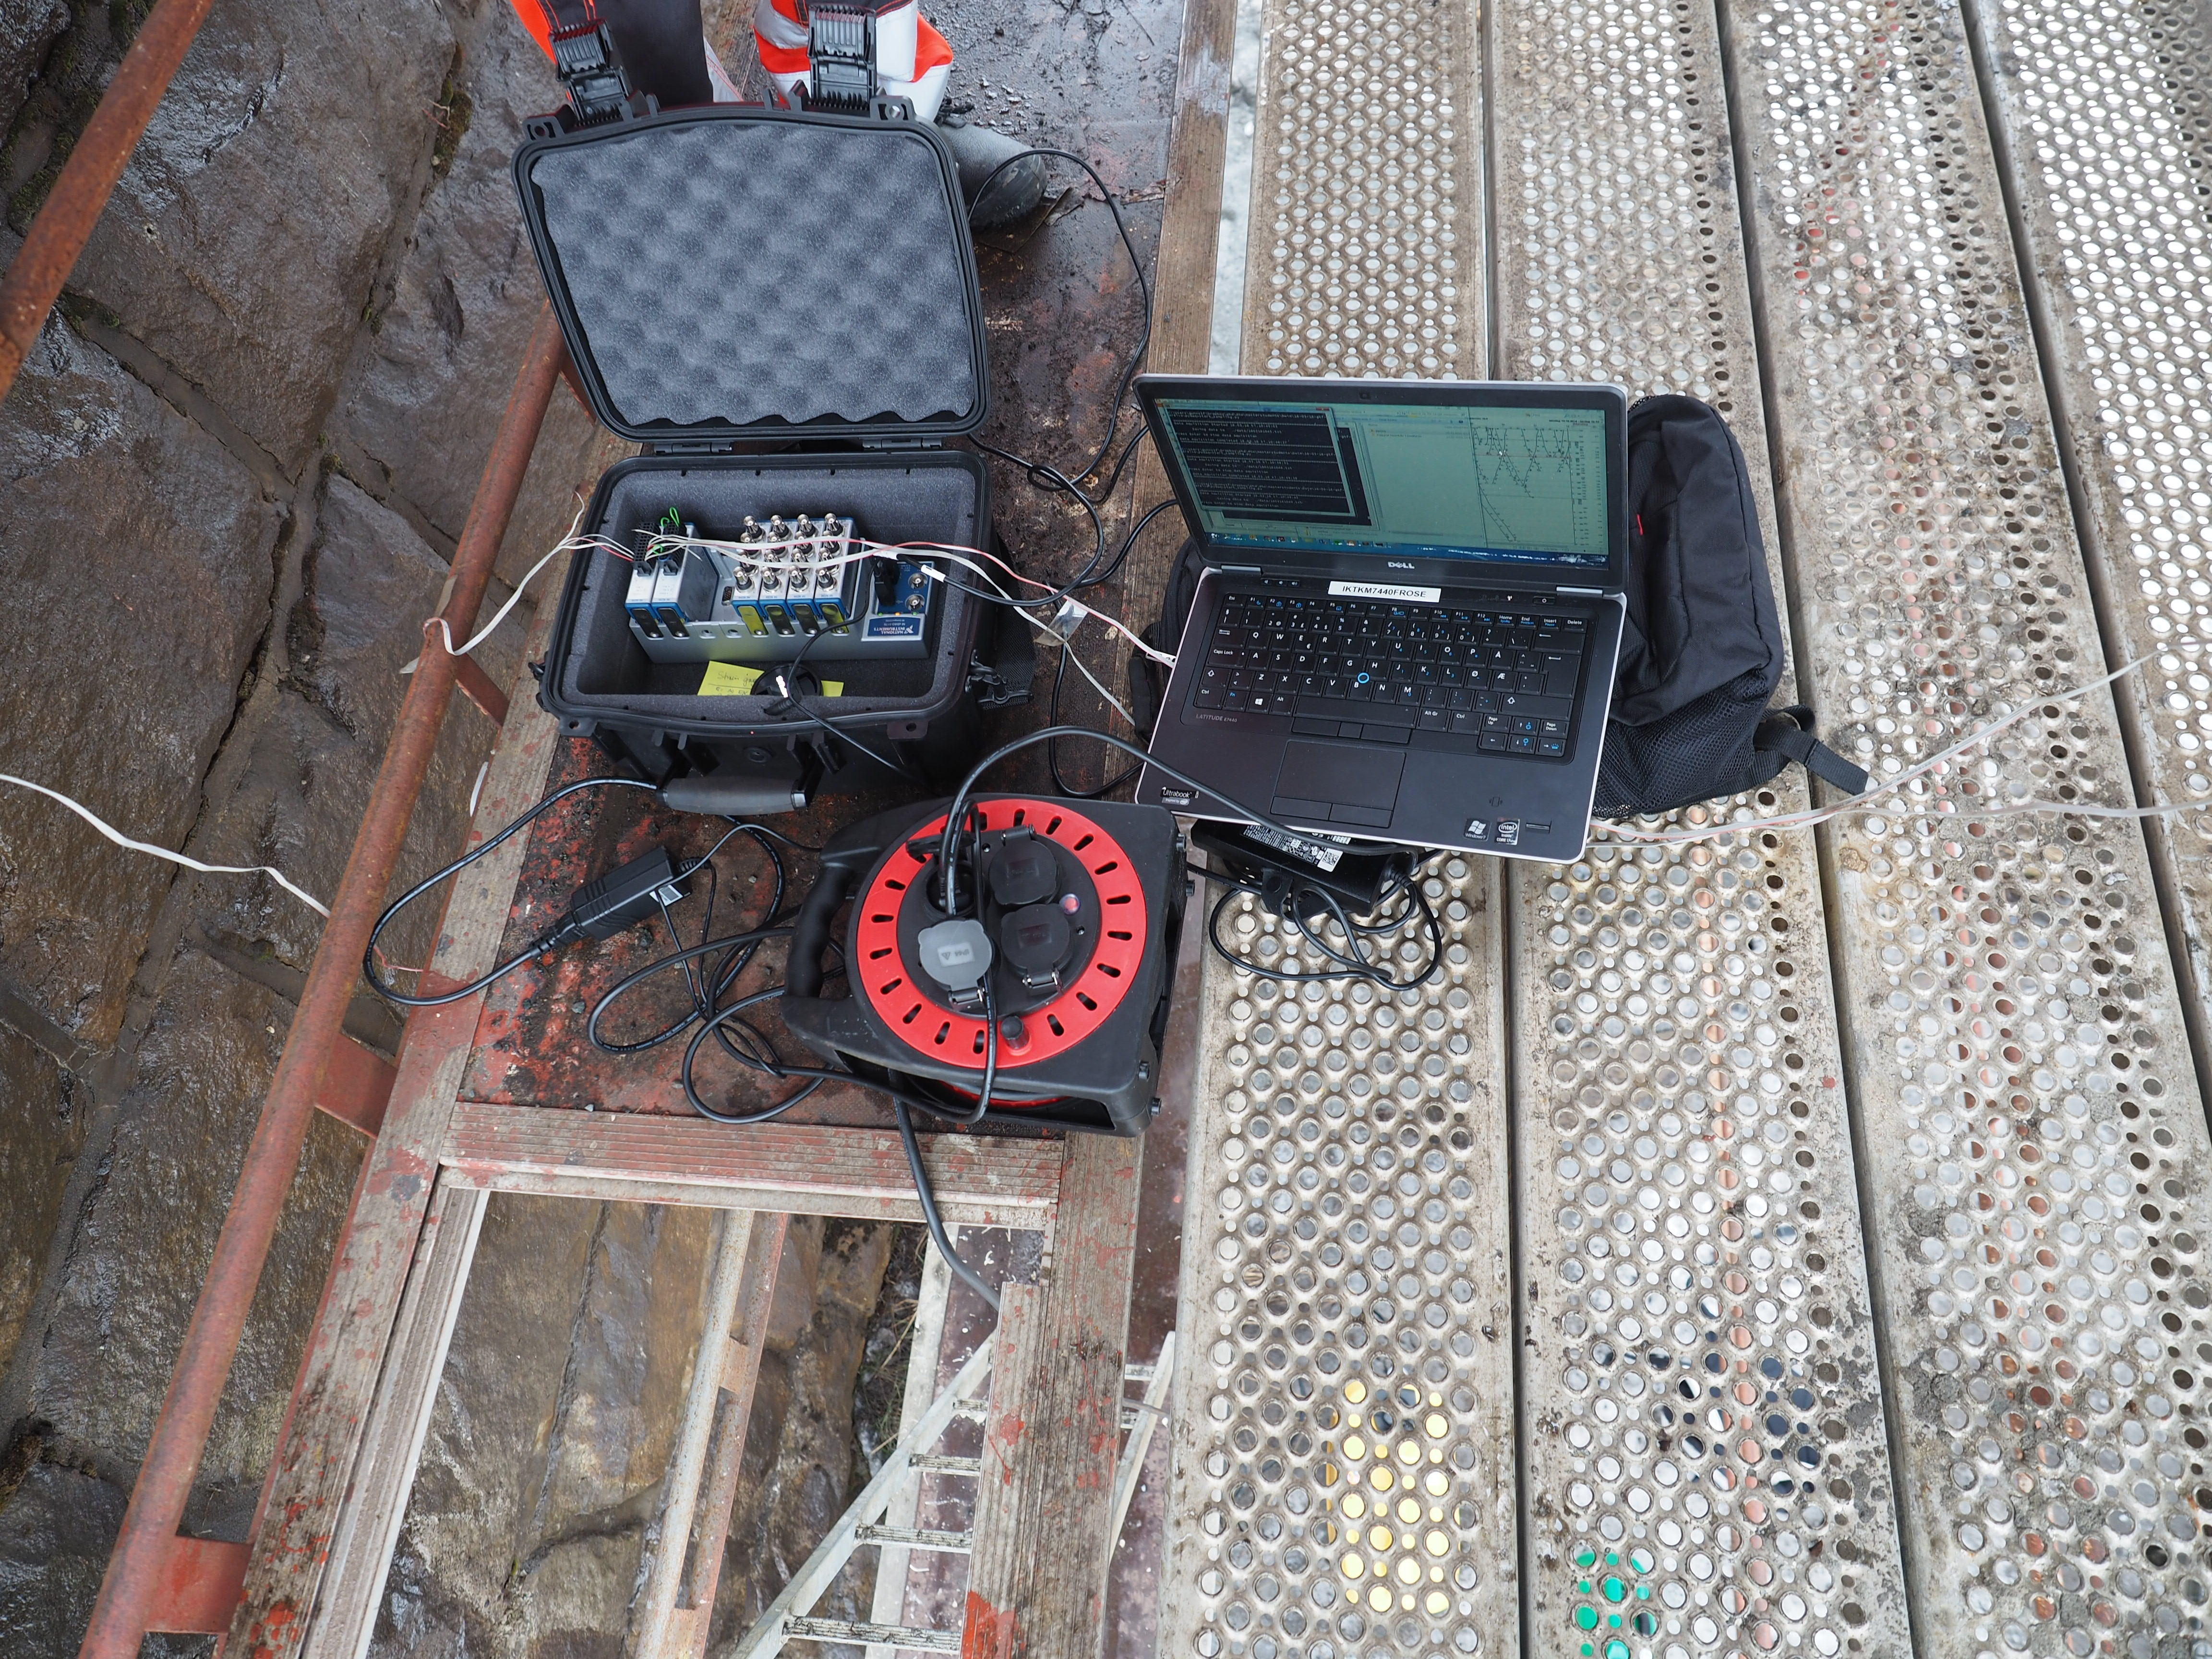
\includegraphics[width=\textwidth]{figures/system_setup}
		\caption{System setup from data gathering at Lerelva}
		\label{fig:instruments}
	\end{subfigure}
	\begin{subfigure}[t]{0.49\textwidth}
    \centering
    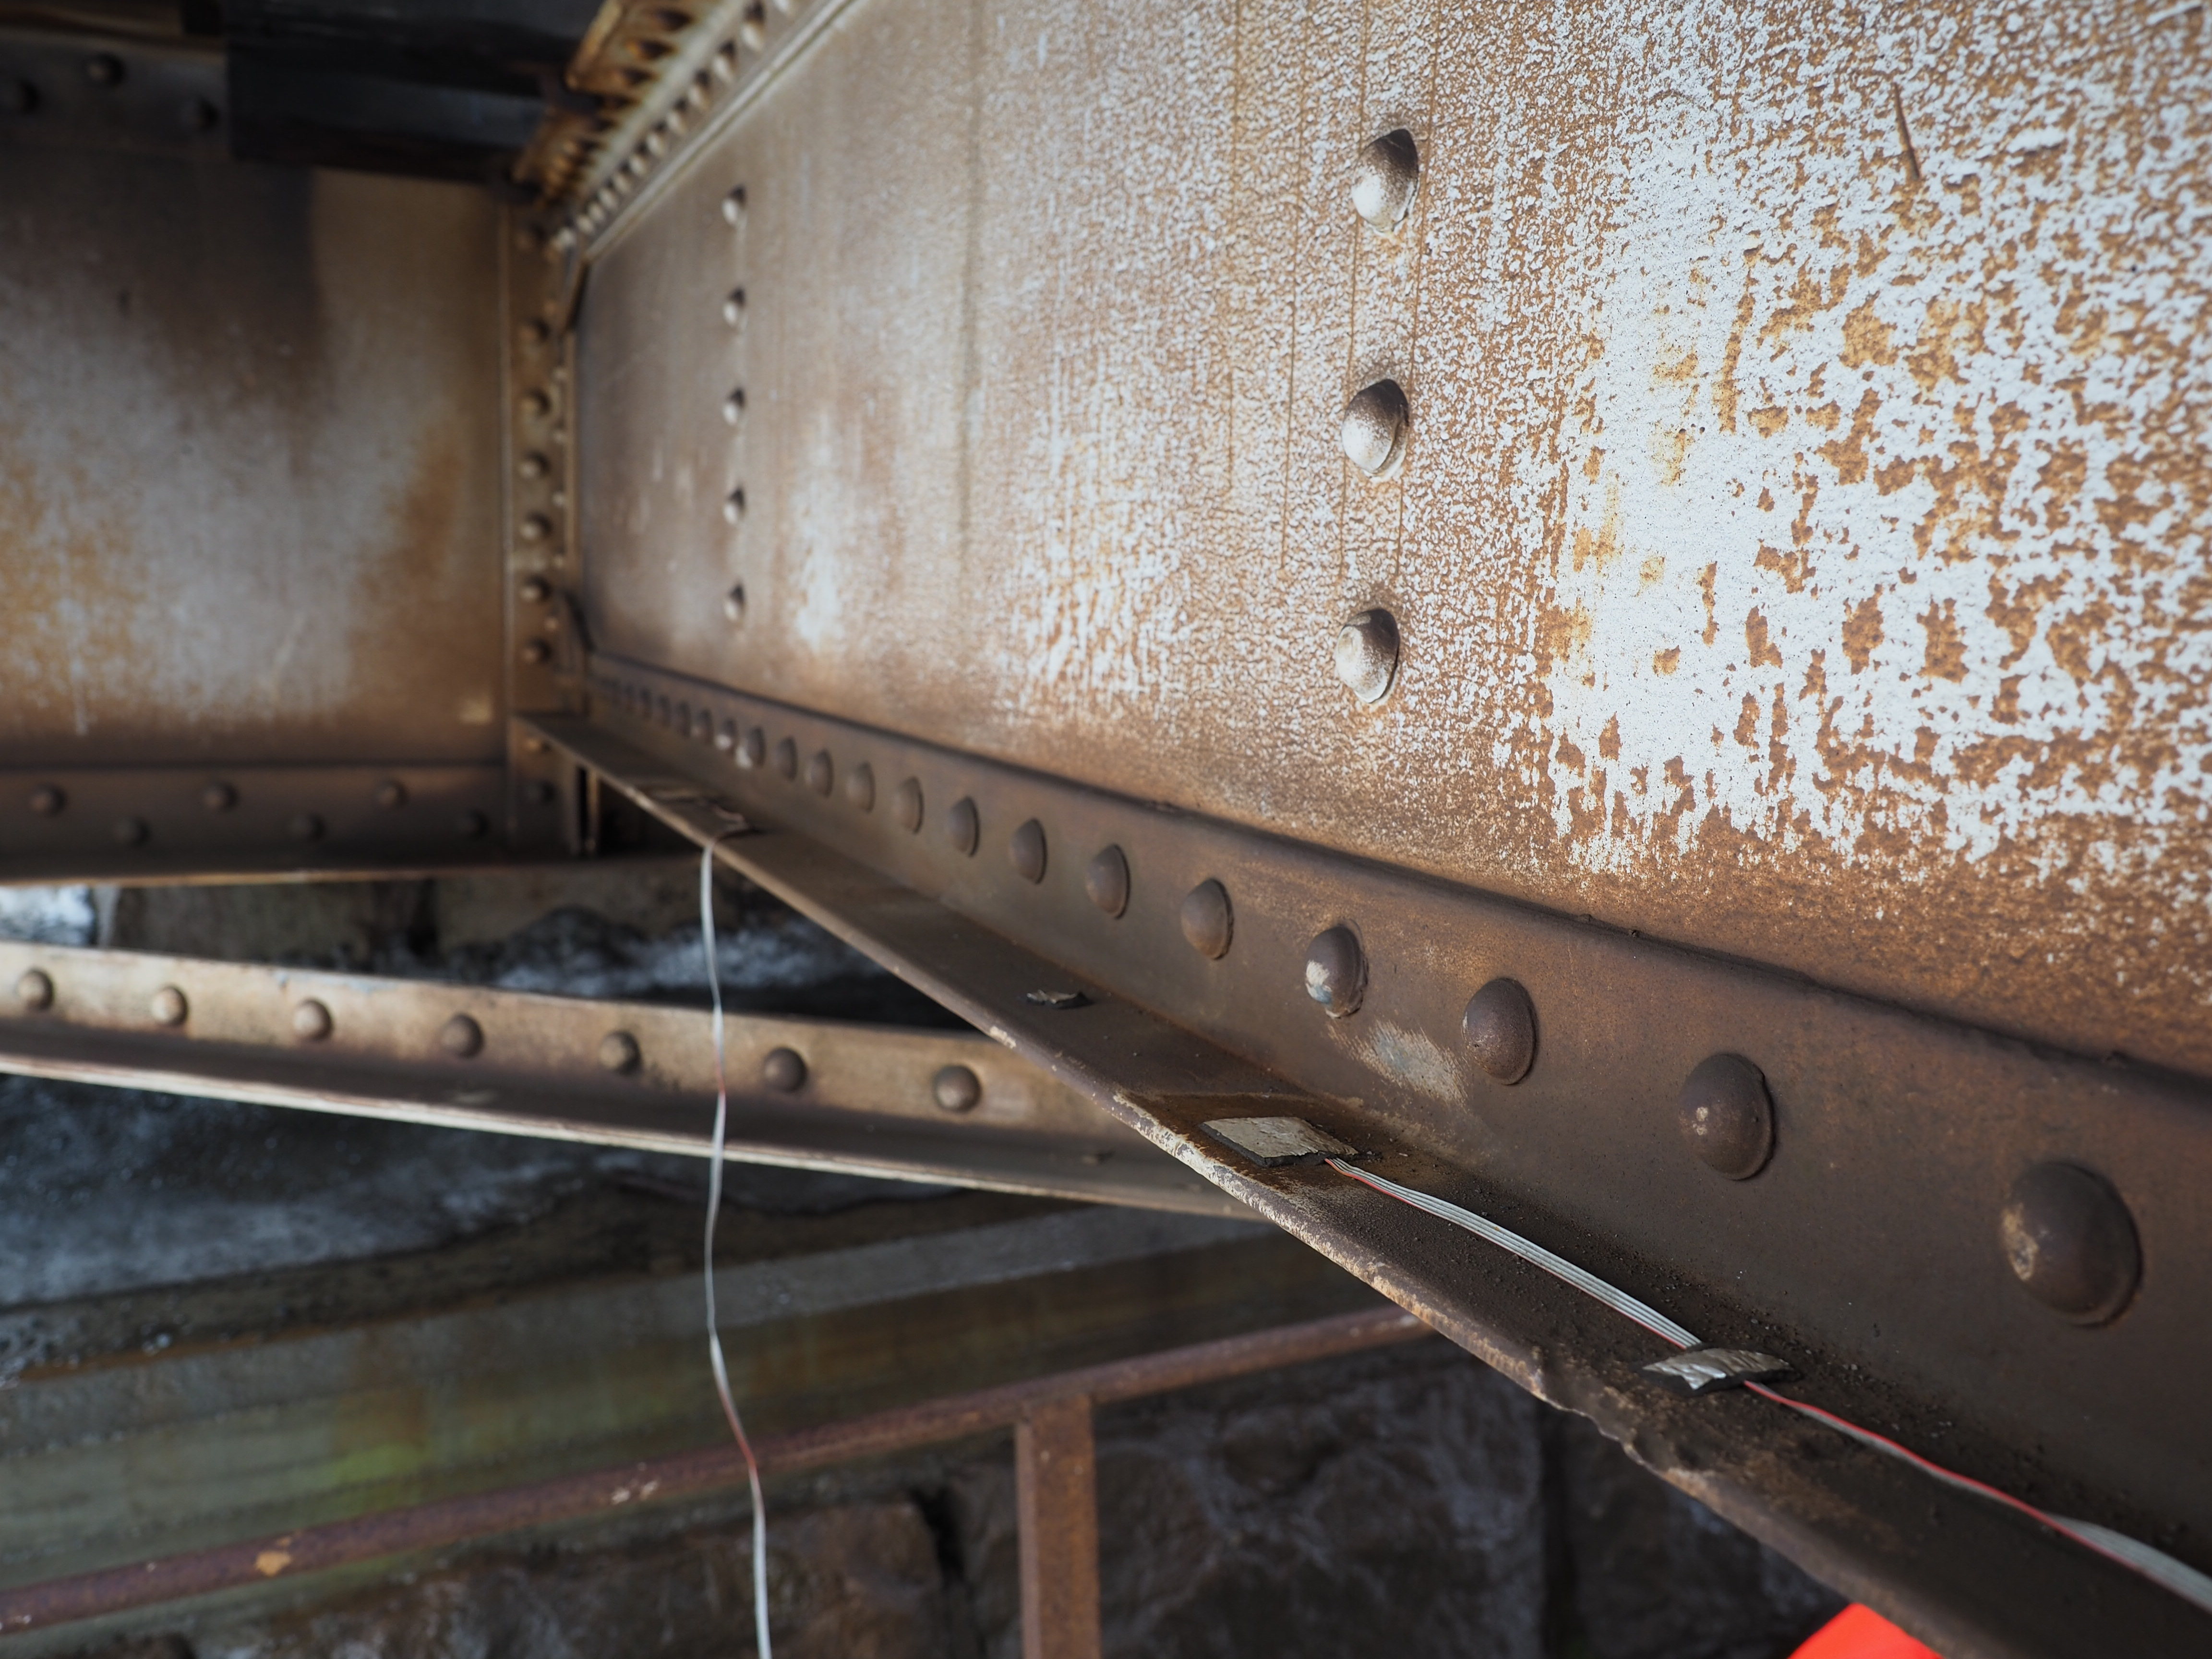
\includegraphics[width=\textwidth]{figures/sensor_placement}
		\caption{Placement of strain gauges on stringer section}
		\label{fig:strain_gauges}
	\end{subfigure}
	\caption{Instruments for aquiring strain data}
	\label{fig:system_setup}
	% 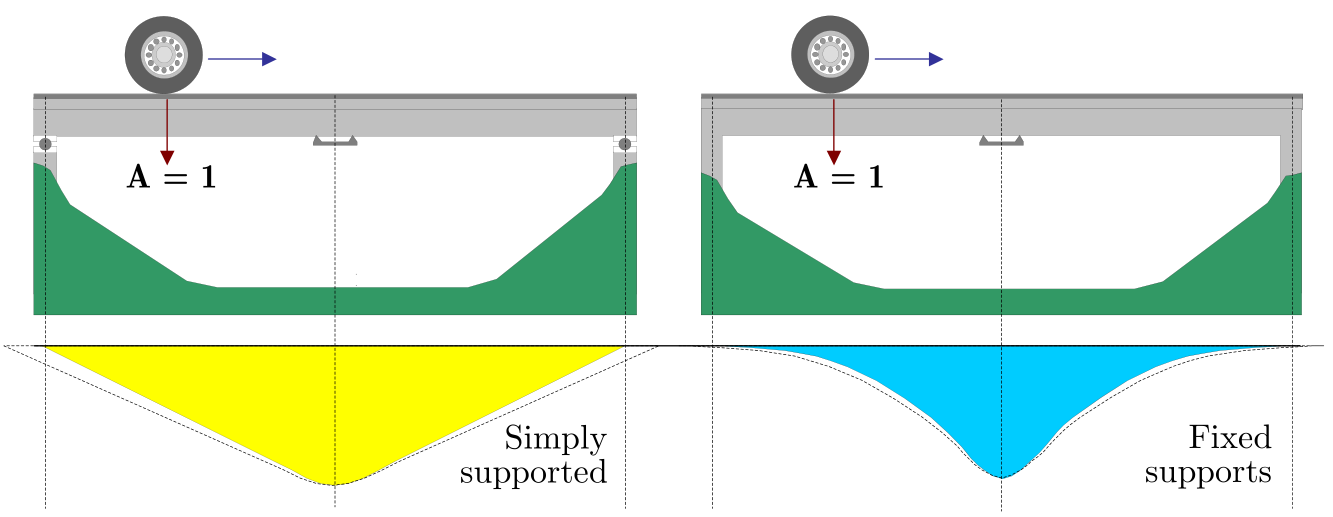
\includegraphics[scale=0.5]{figures/inflLinesQuilligan}
\end{figure}
\begin{figure}[H]
	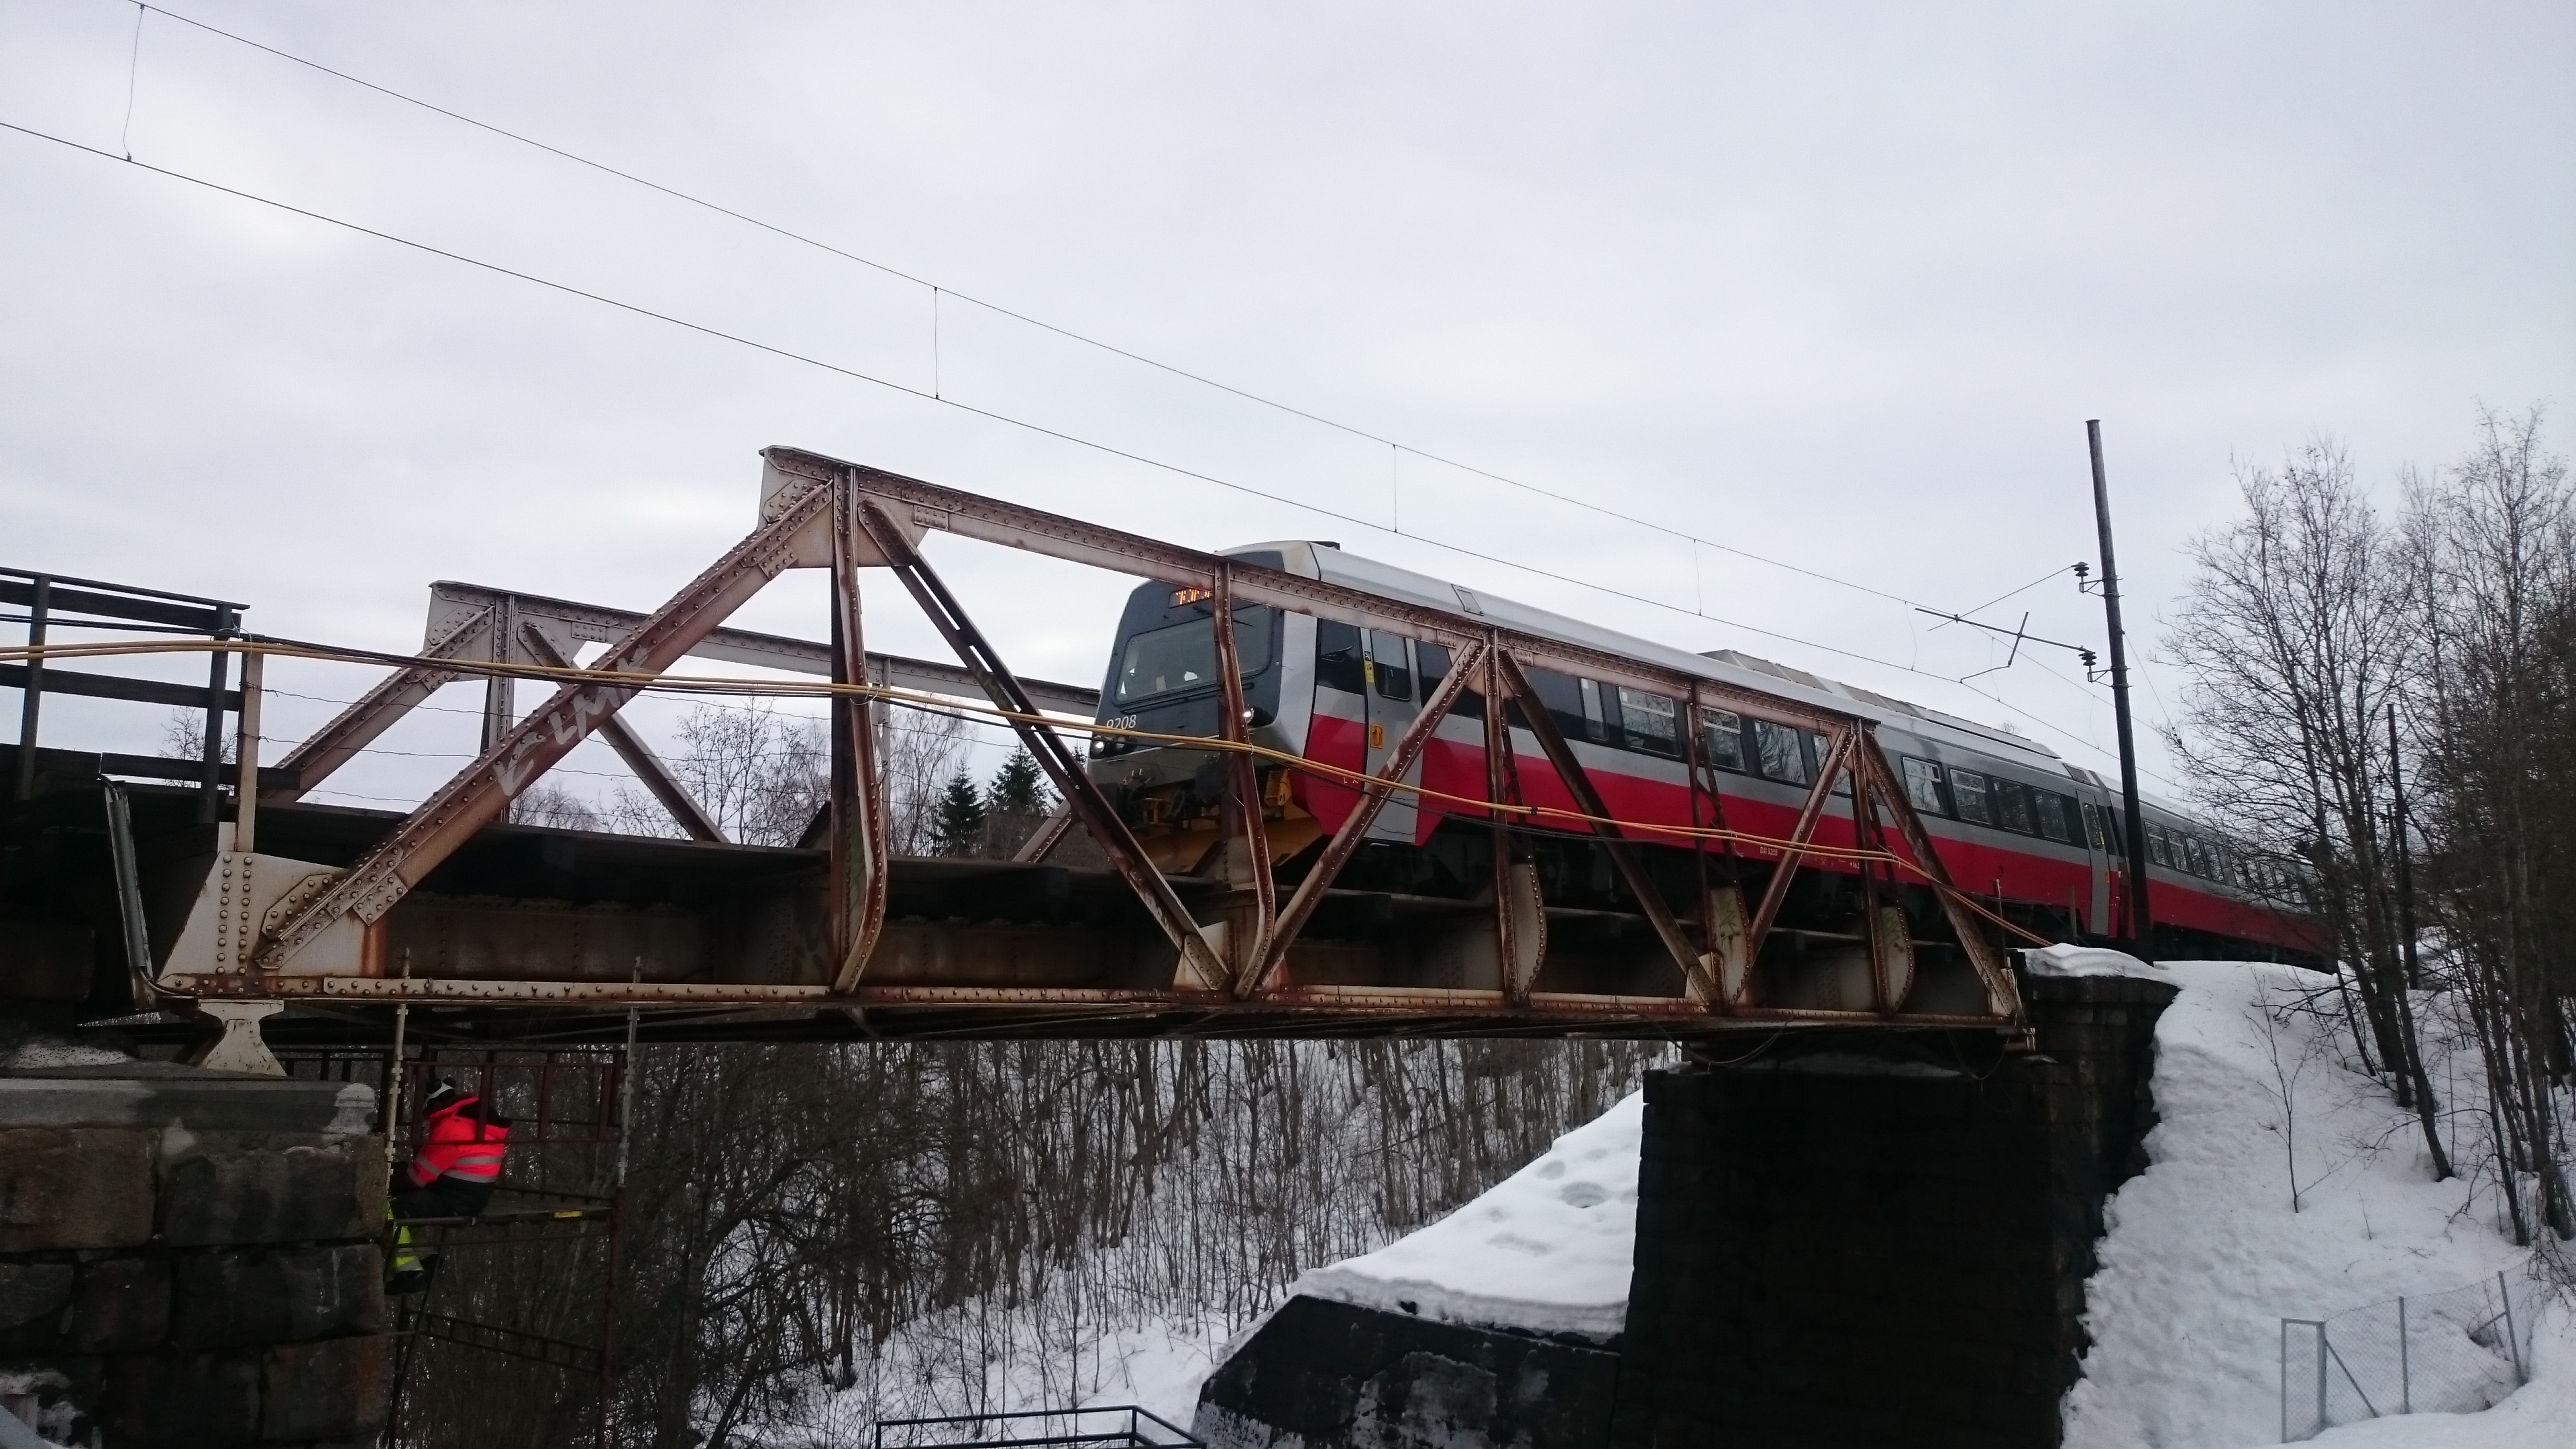
\includegraphics[width=\textwidth]{figures/train_passing.jpg}
	\caption{Lerelva bridge with a train passing over}
	\label{fig:lerelva_bridge}
\end{figure}


\subsection{Testing}
Keywords:
\begin{itemize}
\item Comparing calculated strain with measured strain
\item Perform the same test with a influence line found through the matrix method
\end{itemize}

When performing BWIM with a influence line through the matrix method, the length of the strain signal will require a influence line of a certain length. The exact position where the train begins to influence the bridge is not known due to the special conditions of the Trondheim side support and the dynamic effects in the influence line.
To use the found influence line as correctly as possible, it will be needed to place it in accordance with the provided strain signal.

\subsubsection{Using calculated influence lines}
To perform a standard BWIM calculation, the influence line needs to be aligned correctly with the strain signal, otherwise calculated Axle weights will be based on faulty calculations from solving the system

$A = I_m \textbackslash \varepsilon$ 
(NEEDS TO BE IN THEORY).
The first peak of the strain signal, corresponding to the first axle of the train, should occur at the same location as the peak of the influence line which should be precisely at the strain-gauge/sensor location.
Identifying the first peak of the strain signal is subject to noise which corrupts any reading of peaks in the raw strain signa. Therefore filtering of noise is needed to correctly identify the signals peaks. A trains axle spacings, as seen in \ref{appendix:nsb92} which is the train type of the readings, may consist short spacings. If the axle spacing between two axles are short compared to the bridge, they both influence the signal simoultaneously and the peaks corresponding to the two axles thus lies very close to each other. The filtering can therefore not be to hard or soft, which may result in problems when trying to automate the procedure of identifying axles.
To correctly align the strain signal and influence line, the matlab code used in this thesis first smooths the strain signal to a degree where the desired number of peaks are identifyable before using matlabs findpeaks (REFERENCE THIS) procedure to find the peak locations, like seen in figure \ref{fig:axle_peaks}.
\begin{figure}[htbp]
	\centering
	% This file was created by matlab2tikz.
%
%The latest updates can be retrieved from
%  http://www.mathworks.com/matlabcentral/fileexchange/22022-matlab2tikz-matlab2tikz
%where you can also make suggestions and rate matlab2tikz.
%
\definecolor{mycolor1}{rgb}{0.00000,0.44700,0.74100}%
\definecolor{mycolor2}{rgb}{0.85000,0.32500,0.09800}%
%
\begin{tikzpicture}

  \begin{axis}[%
    width=\textwidth,
    height=0.4\textwidth,
    at={(0\figurewidth,0\figureheight)},
    scale only axis,
    xmin=0,
    xmax=4500,
    xlabel={sensor samples},
    ymin=-5e-05,
    ymax=0.0002,
    ylabel={\varepsilon},
    axis background/.style={fill=white},
    title style={font=\bfseries},
    title={Strain signal},
    legend style={legend cell align=left,align=left,draw=white!15!black}
    ]
    \addplot [color=mycolor1,solid,forget plot]
    table[row sep=crcr]{%
    1	1.07101192055607e-06\\
    2	1.15785473831036e-06\\
    3	1.24695257432971e-06\\
    4	1.33795909976233e-06\\
    5	1.43051062004486e-06\\
    6	1.52422884868125e-06\\
    7	1.61872382133967e-06\\
    8	1.71359692420423e-06\\
    9	1.80844400939035e-06\\
    10	1.90285856936081e-06\\
    11	1.99643494167531e-06\\
    12	2.08877151507188e-06\\
    13	2.17947390782138e-06\\
    14	2.268158089514e-06\\
    15	2.35445341792965e-06\\
    16	2.43800556340617e-06\\
    17	2.51847929414396e-06\\
    18	2.5955610971638e-06\\
    19	2.6689616111522e-06\\
    20	2.73841784917348e-06\\
    21	2.80369519118109e-06\\
    22	2.86458912840487e-06\\
    23	2.92092674400533e-06\\
    24	2.97256791684727e-06\\
    25	3.01940623783136e-06\\
    26	3.06136963090643e-06\\
    27	3.09842067364385e-06\\
    28	3.13055661505934e-06\\
    29	3.15780909119241e-06\\
    30	3.18024354177006e-06\\
    31	3.19795833406382e-06\\
    32	3.21108360277028e-06\\
    33	3.21977981737855e-06\\
    34	3.22423609100969e-06\\
    35	3.2246682470972e-06\\
    36	3.22131666250271e-06\\
    37	3.21444390770554e-06\\
    38	3.20433220654909e-06\\
    39	3.19128073965453e-06\\
    40	3.17560281700575e-06\\
    41	3.15762294635929e-06\\
    42	3.13767382502496e-06\\
    43	3.11609328319061e-06\\
    44	3.0932212073238e-06\\
    45	3.0693964722678e-06\\
    46	3.04495391046257e-06\\
    47	3.02022134626329e-06\\
    48	2.99551672260636e-06\\
    49	2.97114534629135e-06\\
    50	2.94739727691906e-06\\
    51	2.92454488306264e-06\\
    52	2.9028405875642e-06\\
    53	2.88251482196242e-06\\
    54	2.8637742079848e-06\\
    55	2.84679998180184e-06\\
    56	2.8317466743631e-06\\
    57	2.81874105863844e-06\\
    58	2.80788137199758e-06\\
    59	2.7992368193022e-06\\
    60	2.79284735958379e-06\\
    61	2.78872377646215e-06\\
    62	2.78684802975203e-06\\
    63	2.7871738830346e-06\\
    64	2.78962779935979e-06\\
    65	2.79411009472477e-06\\
    66	2.80049633656153e-06\\
    67	2.80863897219052e-06\\
    68	2.81836917007551e-06\\
    69	2.82949885476947e-06\\
    70	2.84182291468976e-06\\
    71	2.85512156031882e-06\\
    72	2.86916280910931e-06\\
    73	2.88370507229044e-06\\
    74	2.89849981793621e-06\\
    75	2.91329428407222e-06\\
    76	2.92783421526998e-06\\
    77	2.94186659611012e-06\\
    78	2.95514235508501e-06\\
    79	2.96741901295683e-06\\
    80	2.9784632502808e-06\\
    81	2.98805336974028e-06\\
    82	2.99598163010627e-06\\
    83	3.00205643001963e-06\\
    84	3.00610432138358e-06\\
    85	3.00797183392982e-06\\
    86	3.00752709446612e-06\\
    87	3.00466122640742e-06\\
    88	2.9992895174123e-06\\
    89	2.99135234527266e-06\\
    90	2.98081585461111e-06\\
    91	2.96767237940475e-06\\
    92	2.95194060885043e-06\\
    93	2.933665496592e-06\\
    94	2.91291791581728e-06\\
    95	2.88979406517949e-06\\
    96	2.86441463288027e-06\\
    97	2.83692372854414e-06\\
    98	2.80748759469876e-06\\
    99	2.77629311172744e-06\\
    100	2.74354611206273e-06\\
    101	2.70946952112381e-06\\
    102	2.67430134405017e-06\\
    103	2.6382925186351e-06\\
    104	2.60170465600364e-06\\
    105	2.5648076915002e-06\\
    106	2.52787746894345e-06\\
    107	2.4911932818658e-06\\
    108	2.45503539557809e-06\\
    109	2.41968257388664e-06\\
    110	2.38540963404192e-06\\
    111	2.35248505301926e-06\\
    112	2.32116864752913e-06\\
    113	2.29170934923572e-06\\
    114	2.26434309554024e-06\\
    115	2.23929085496942e-06\\
    116	2.21675680471769e-06\\
    117	2.19692667623817e-06\\
    118	2.17996628298069e-06\\
    119	2.16602024245452e-06\\
    120	2.15521090276914e-06\\
    121	2.14763748169876e-06\\
    122	2.14337542414927e-06\\
    123	2.142475981699e-06\\
    124	2.1449660156634e-06\\
    125	2.15084802291733e-06\\
    126	2.16010038152303e-06\\
    127	2.17267781107562e-06\\
    128	2.18851204061427e-06\\
    129	2.20751267497674e-06\\
    130	2.22956824861435e-06\\
    131	2.25454745415543e-06\\
    132	2.28230053142016e-06\\
    133	2.31266080116753e-06\\
    134	2.34544632660512e-06\\
    135	2.38046168462887e-06\\
    136	2.41749982789026e-06\\
    137	2.4563440181204e-06\\
    138	2.49676981067939e-06\\
    139	2.53854707004721e-06\\
    140	2.58144199593128e-06\\
    141	2.62521913983302e-06\\
    142	2.66964339228794e-06\\
    143	2.71448192156572e-06\\
    144	2.75950604538049e-06\\
    145	2.80449301810664e-06\\
    146	2.849227717112e-06\\
    147	2.89350421309301e-06\\
    148	2.93712721071385e-06\\
    149	2.97991334739261e-06\\
    150	3.02169233973116e-06\\
    151	3.06230796882751e-06\\
    152	3.10161889752512e-06\\
    153	3.13949931452059e-06\\
    154	3.17583940215105e-06\\
    155	3.21054562659395e-06\\
    156	3.24354085111495e-06\\
    157	3.27476427487458e-06\\
    158	3.30417120163105e-06\\
    159	3.33173264443684e-06\\
    160	3.35743477410208e-06\\
    161	3.38127822077042e-06\\
    162	3.40327723940982e-06\\
    163	3.42345875134288e-06\\
    164	3.44186127512136e-06\\
    165	3.45853376106956e-06\\
    166	3.47353434467925e-06\\
    167	3.48692903471944e-06\\
    168	3.49879035242805e-06\\
    169	3.5091959384713e-06\\
    170	3.51822714449095e-06\\
    171	3.5259676260078e-06\\
    172	3.53250195321596e-06\\
    173	3.53791425578838e-06\\
    174	3.5422869172278e-06\\
    175	3.54569933354472e-06\\
    176	3.54822675013577e-06\\
    177	3.54993918968282e-06\\
    178	3.55090048270746e-06\\
    179	3.55116741111083e-06\\
    180	3.55078897362202e-06\\
    181	3.54980578058266e-06\\
    182	3.54824958392986e-06\\
    183	3.5461429466221e-06\\
    184	3.54349905409902e-06\\
    185	3.54032166869701e-06\\
    186	3.53660522627483e-06\\
    187	3.5323350726566e-06\\
    188	3.5274878358898e-06\\
    189	3.52203192876262e-06\\
    190	3.51592817454412e-06\\
    191	3.50913054751629e-06\\
    192	3.5015870185782e-06\\
    193	3.4932404950277e-06\\
    194	3.48402984258126e-06\\
    195	3.4738909767874e-06\\
    196	3.46275801023222e-06\\
    197	3.45056444133535e-06\\
    198	3.43724437009632e-06\\
    199	3.42273372587983e-06\\
    200	3.40697149222425e-06\\
    201	3.38990091372363e-06\\
    202	3.37147067026538e-06\\
    203	3.35163600430252e-06\\
    204	3.33035978739484e-06\\
    205	3.30761351296058e-06\\
    206	3.28337820303155e-06\\
    207	3.2576452177896e-06\\
    208	3.23041695776933e-06\\
    209	3.20170744982954e-06\\
    210	3.17154280930843e-06\\
    211	3.13996157217217e-06\\
    212	3.10701489242575e-06\\
    213	3.07276660156443e-06\\
    214	3.03729312838564e-06\\
    215	3.00068327903762e-06\\
    216	2.96303787873738e-06\\
    217	2.92446927812668e-06\\
    218	2.88510072873567e-06\\
    219	2.8450656334738e-06\\
    220	2.80450667944871e-06\\
    221	2.76357486171299e-06\\
    222	2.72242840774158e-06\\
    223	2.68123161353551e-06\\
    224	2.64015360321941e-06\\
    225	2.59936702484188e-06\\
    226	2.55904669578693e-06\\
    227	2.51936821175886e-06\\
    228	2.48050653370193e-06\\
    229	2.44263456725937e-06\\
    230	2.40592174945947e-06\\
    231	2.37053265724016e-06\\
    232	2.3366256521883e-06\\
    233	2.30435157547968e-06\\
    234	2.27385250646397e-06\\
    235	2.24526059765286e-06\\
    236	2.21869699804667e-06\\
    237	2.19427087578467e-06\\
    238	2.17207855003709e-06\\
    239	2.1522027408848e-06\\
    240	2.13471194466955e-06\\
    241	2.11965994095553e-06\\
    242	2.10708543583914e-06\\
    243	2.09701184489166e-06\\
    244	2.08944721753616e-06\\
    245	2.08438430316093e-06\\
    246	2.08180075777392e-06\\
    247	2.08165948852235e-06\\
    248	2.08390913195349e-06\\
    249	2.08848466049559e-06\\
    250	2.09530811030273e-06\\
    251	2.10428942235178e-06\\
    252	2.11532738751598e-06\\
    253	2.12831068527973e-06\\
    254	2.14311900481459e-06\\
    255	2.15962423631818e-06\\
    256	2.17769171983233e-06\\
    257	2.19718153821281e-06\\
    258	2.21794984052597e-06\\
    259	2.23985018189991e-06\\
    260	2.26273486576365e-06\\
    261	2.28645627446633e-06\\
    262	2.31086817447878e-06\\
    263	2.33582698274005e-06\\
    264	2.36119298121555e-06\\
    265	2.38683146737756e-06\\
    266	2.41261382909249e-06\\
    267	2.43841853329783e-06\\
    268	2.46413201885971e-06\\
    269	2.48964948511261e-06\\
    270	2.51487556878118e-06\\
    271	2.53972490325665e-06\\
    272	2.56412255553438e-06\\
    273	2.58800433749805e-06\\
    274	2.61131698964593e-06\\
    275	2.63401823677874e-06\\
    276	2.65607671659242e-06\\
    277	2.67747178352556e-06\\
    278	2.69819319158612e-06\\
    279	2.71824066120887e-06\\
    280	2.73762333646164e-06\\
    281	2.75635914010726e-06\\
    282	2.77447403513046e-06\\
    283	2.79200120234026e-06\\
    284	2.80898014454729e-06\\
    285	2.82545572858569e-06\\
    286	2.84147717708881e-06\\
    287	2.85709702243231e-06\\
    288	2.87237003562175e-06\\
    289	2.88735214312121e-06\\
    290	2.90209934469009e-06\\
    291	2.91666664522219e-06\\
    292	2.93110701335865e-06\\
    293	2.94547037928325e-06\\
    294	2.95980268360538e-06\\
    295	2.97414498860084e-06\\
    296	2.98853266231934e-06\\
    297	3.00299464519017e-06\\
    298	3.01755280777342e-06\\
    299	3.03222140722422e-06\\
    300	3.04700664887516e-06\\
    301	3.06190635810887e-06\\
    302	3.07690976640419e-06\\
    303	3.09199741410881e-06\\
    304	3.10714117113457e-06\\
    305	3.12230437540221e-06\\
    306	3.13744208749938e-06\\
    307	3.15250145866907e-06\\
    308	3.16742220793535e-06\\
    309	3.18213720291112e-06\\
    310	3.19657313763345e-06\\
    311	3.21065129964912e-06\\
    312	3.22428841753932e-06\\
    313	3.23739757913932e-06\\
    314	3.24988920988485e-06\\
    315	3.26167210001572e-06\\
    316	3.27265446879077e-06\\
    317	3.28274505342695e-06\\
    318	3.29185421017388e-06\\
    319	3.29989501477402e-06\\
    320	3.30678434954283e-06\\
    321	3.31244396443067e-06\\
    322	3.31680149969921e-06\\
    323	3.31979145825312e-06\\
    324	3.32135611621458e-06\\
    325	3.32144636099944e-06\\
    326	3.32002244694886e-06\\
    327	3.31705465947711e-06\\
    328	3.31252387970406e-06\\
    329	3.30642204264028e-06\\
    330	3.29875248317075e-06\\
    331	3.28953016532553e-06\\
    332	3.27878179161982e-06\\
    333	3.26654579057761e-06\\
    334	3.25287218190486e-06\\
    335	3.23782232013895e-06\\
    336	3.22146851895162e-06\\
    337	3.20389355961083e-06\\
    338	3.18519008839591e-06\\
    339	3.16545990899717e-06\\
    340	3.14481317710074e-06\\
    341	3.12336750544939e-06\\
    342	3.10124698866818e-06\\
    343	3.07858115803886e-06\\
    344	3.05550387718788e-06\\
    345	3.03215219031344e-06\\
    346	3.00866513510672e-06\\
    347	2.98518253291736e-06\\
    348	2.96184376896868e-06\\
    349	2.93878657554065e-06\\
    350	2.91614583100656e-06\\
    351	2.89405238743499e-06\\
    352	2.87263193915129e-06\\
    353	2.85200394419792e-06\\
    354	2.8322806100447e-06\\
    355	2.81356595418607e-06\\
    356	2.79595494942762e-06\\
    357	2.77953276272353e-06\\
    358	2.7643740953843e-06\\
    359	2.75054263134571e-06\\
    360	2.73809059898888e-06\\
    361	2.72705845073624e-06\\
    362	2.71747466333951e-06\\
    363	2.70935566043332e-06\\
    364	2.70270585756968e-06\\
    365	2.69751782858815e-06\\
    366	2.69377259083031e-06\\
    367	2.69144000539028e-06\\
    368	2.69047928731864e-06\\
    369	2.69083961948368e-06\\
    370	2.69246086264967e-06\\
    371	2.6952743532748e-06\\
    372	2.69920377957065e-06\\
    373	2.70416612551249e-06\\
    374	2.71007267175463e-06\\
    375	2.71683004179714e-06\\
    376	2.72434128127401e-06\\
    377	2.73250695789707e-06\\
    378	2.74122626939543e-06\\
    379	2.75039814674198e-06\\
    380	2.75992234005452e-06\\
    381	2.76970047480137e-06\\
    382	2.77963706632511e-06\\
    383	2.78964048121932e-06\\
    384	2.7996238347478e-06\\
    385	2.80950581427446e-06\\
    386	2.8192114195669e-06\\
    387	2.82867261183788e-06\\
    388	2.83782886448543e-06\\
    389	2.84662760966915e-06\\
    390	2.8550245761094e-06\\
    391	2.86298401479661e-06\\
    392	2.87047881064041e-06\\
    393	2.87749047945538e-06\\
    394	2.88400905105453e-06\\
    395	2.89003284059094e-06\\
    396	2.89556811163315e-06\\
    397	2.90062863576765e-06\\
    398	2.9052351547745e-06\\
    399	2.90941475260891e-06\\
    400	2.91320014552346e-06\\
    401	2.91662889967437e-06\\
    402	2.91974258645581e-06\\
    403	2.92258588658853e-06\\
    404	2.92520565464421e-06\\
    405	2.92764995620617e-06\\
    406	2.92996709024378e-06\\
    407	2.93220460950722e-06\\
    408	2.93440835182834e-06\\
    409	2.93662149513936e-06\\
    410	2.93888364879517e-06\\
    411	2.94122999340911e-06\\
    412	2.94369048088833e-06\\
    413	2.94628910568998e-06\\
    414	2.94904325751976e-06\\
    415	2.95196316476878e-06\\
    416	2.95505143694139e-06\\
    417	2.95830271318014e-06\\
    418	2.96170342275367e-06\\
    419	2.96523166205503e-06\\
    420	2.96885719127507e-06\\
    421	2.97254155248546e-06\\
    422	2.97623830940079e-06\\
    423	2.97989340761253e-06\\
    424	2.98344565260809e-06\\
    425	2.98682730142921e-06\\
    426	2.98996476240076e-06\\
    427	2.99277939598693e-06\\
    428	2.99518840852907e-06\\
    429	2.99710582939773e-06\\
    430	2.99844356096952e-06\\
    431	2.9991124898284e-06\\
    432	2.99902364670531e-06\\
    433	2.99808940191937e-06\\
    434	2.99622468247854e-06\\
    435	2.99334819654656e-06\\
    436	2.98938365069129e-06\\
    437	2.9842609452027e-06\\
    438	2.97791733281036e-06\\
    439	2.97029852634023e-06\\
    440	2.96135974122831e-06\\
    441	2.95106665935258e-06\\
    442	2.93939630134874e-06\\
    443	2.92633779543349e-06\\
    444	2.91189303176447e-06\\
    445	2.89607719250657e-06\\
    446	2.87891914903972e-06\\
    447	2.86046171912117e-06\\
    448	2.84076177829027e-06\\
    449	2.81989022135912e-06\\
    450	2.79793177145581e-06\\
    451	2.77498463575548e-06\\
    452	2.75116000873335e-06\\
    453	2.72658142548434e-06\\
    454	2.70138396935561e-06\\
    455	2.67571333981231e-06\\
    456	2.64972478808714e-06\\
    457	2.6235819297275e-06\\
    458	2.59745544463623e-06\\
    459	2.57152167658474e-06\\
    460	2.54596114544277e-06\\
    461	2.52095698650466e-06\\
    462	2.49669333228201e-06\\
    463	2.47335365296566e-06\\
    464	2.45111907242396e-06\\
    465	2.43016667709284e-06\\
    466	2.41066783541596e-06\\
    467	2.39278654560725e-06\\
    468	2.37667782942996e-06\\
    469	2.36248618941405e-06\\
    470	2.35034414646848e-06\\
    471	2.34037087419172e-06\\
    472	2.33267094534512e-06\\
    473	2.32733320493842e-06\\
    474	2.32442978319452e-06\\
    475	2.32401526032192e-06\\
    476	2.32612599354016e-06\\
    477	2.33077961519452e-06\\
    478	2.33797470907199e-06\\
    479	2.34769067021354e-06\\
    480	2.35988775162413e-06\\
    481	2.37450729933269e-06\\
    482	2.39147217526844e-06\\
    483	2.41068736542119e-06\\
    484	2.43204076876102e-06\\
    485	2.4554041604283e-06\\
    486	2.4806343207925e-06\\
    487	2.50757432013628e-06\\
    488	2.53605494697009e-06\\
    489	2.5658962663459e-06\\
    490	2.59690929302909e-06\\
    491	2.62889776302781e-06\\
    492	2.66165998578357e-06\\
    493	2.69499075830741e-06\\
    494	2.72868332172003e-06\\
    495	2.7625313400282e-06\\
    496	2.79633088055485e-06\\
    497	2.82988237524054e-06\\
    498	2.86299254205732e-06\\
    499	2.89547624601945e-06\\
    500	2.92715827974193e-06\\
    501	2.95787504418389e-06\\
    502	2.98747611111224e-06\\
    503	3.01582564992596e-06\\
    504	3.0428037027828e-06\\
    505	3.06830729345466e-06\\
    506	3.09225135699214e-06\\
    507	3.11456947908694e-06\\
    508	3.13521443596388e-06\\
    509	3.15415852769323e-06\\
    510	3.17139369996879e-06\\
    511	3.18693145162364e-06\\
    512	3.20080252743167e-06\\
    513	3.21305639804574e-06\\
    514	3.22376053122694e-06\\
    515	3.23299946079853e-06\\
    516	3.24087366199226e-06\\
    517	3.24749824401384e-06\\
    518	3.25300147271933e-06\\
    519	3.25752313823991e-06\\
    520	3.26121278419809e-06\\
    521	3.26422781680165e-06\\
    522	3.2667315135666e-06\\
    523	3.26889095268644e-06\\
    524	3.27087488511881e-06\\
    525	3.27285157228939e-06\\
    526	3.27498661290324e-06\\
    527	3.27744078270048e-06\\
    528	3.28036791108744e-06\\
    529	3.28391281841531e-06\\
    530	3.28820933726238e-06\\
    531	3.2933784404086e-06\\
    532	3.29952649727389e-06\\
    533	3.30674367943398e-06\\
    534	3.31510253443882e-06\\
    535	3.3246567455511e-06\\
    536	3.33544009321126e-06\\
    537	3.34746563203851e-06\\
    538	3.36072509501308e-06\\
    539	3.37518853417475e-06\\
    540	3.39080420474119e-06\\
    541	3.40749869701833e-06\\
    542	3.42517731787289e-06\\
    543	3.44372472088888e-06\\
    544	3.46300578166385e-06\\
    545	3.48286671204382e-06\\
    546	3.50313640447843e-06\\
    547	3.52362799512492e-06\\
    548	3.54414063187009e-06\\
    549	3.5644614311017e-06\\
    550	3.58436760486607e-06\\
    551	3.60362873802673e-06\\
    552	3.62200919320853e-06\\
    553	3.63927061969594e-06\\
    554	3.65517454107108e-06\\
    555	3.66948499524389e-06\\
    556	3.68197119965817e-06\\
    557	3.69241021386208e-06\\
    558	3.70058957132397e-06\\
    559	3.70630985235382e-06\\
    560	3.7093871702655e-06\\
    561	3.70965554348198e-06\\
    562	3.70696912714317e-06\\
    563	3.70120427891669e-06\\
    564	3.69226143512825e-06\\
    565	3.68006677500667e-06\\
    566	3.66457365276413e-06\\
    567	3.6457637793889e-06\\
    568	3.62364813839365e-06\\
    569	3.59826762231483e-06\\
    570	3.56969337947564e-06\\
    571	3.53802686337621e-06\\
    572	3.50339958003479e-06\\
    573	3.46597253164185e-06\\
    574	3.42593535797546e-06\\
    575	3.38350518012826e-06\\
    576	3.33892515418397e-06\\
    577	3.29246274552175e-06\\
    578	3.24440773738692e-06\\
    579	3.19506999021897e-06\\
    580	3.14477697093873e-06\\
    581	3.09387107393776e-06\\
    582	3.04270675785964e-06\\
    583	2.9916475243849e-06\\
    584	2.94106276710838e-06\\
    585	2.89132452020772e-06\\
    586	2.84280413792482e-06\\
    587	2.79586893690365e-06\\
    588	2.75087883413448e-06\\
    589	2.70818301363607e-06\\
    590	2.66811665505764e-06\\
    591	2.63099775709798e-06\\
    592	2.59712408802009e-06\\
    593	2.56677029458947e-06\\
    594	2.54018519949065e-06\\
    595	2.51758931568803e-06\\
    596	2.4991726043099e-06\\
    597	2.48509250046278e-06\\
    598	2.47547222894888e-06\\
    599	2.47039942918295e-06\\
    600	2.46992510571412e-06\\
    601	2.47406291767798e-06\\
    602	2.48278881726606e-06\\
    603	2.49604104393487e-06\\
    604	2.51372047761758e-06\\
    605	2.53569135068243e-06\\
    606	2.56178231483884e-06\\
    607	2.59178785565939e-06\\
    608	2.62547004389997e-06\\
    609	2.66256060939635e-06\\
    610	2.70276332002847e-06\\
    611	2.74575664510646e-06\\
    612	2.79119667958023e-06\\
    613	2.83872030273442e-06\\
    614	2.88794854253496e-06\\
    615	2.93849011456712e-06\\
    616	2.98994510257251e-06\\
    617	3.04190874597518e-06\\
    618	3.09397529850292e-06\\
    619	3.14574192107455e-06\\
    620	3.19681257154735e-06\\
    621	3.24680185371092e-06\\
    622	3.29533878807785e-06\\
    623	3.3420704675568e-06\\
    624	3.38666556200007e-06\\
    625	3.42881763688479e-06\\
    626	3.46824825300653e-06\\
    627	3.50470981602066e-06\\
    628	3.53798814694315e-06\\
    629	3.56790474729672e-06\\
    630	3.59431873543745e-06\\
    631	3.61712843369299e-06\\
    632	3.63627258925631e-06\\
    633	3.65173121527805e-06\\
    634	3.6635260422501e-06\\
    635	3.67172057353804e-06\\
    636	3.67641974276341e-06\\
    637	3.67776917462053e-06\\
    638	3.67595405459683e-06\\
    639	3.67119761691345e-06\\
    640	3.66375926377409e-06\\
    641	3.65393233266651e-06\\
    642	3.64204153196742e-06\\
    643	3.62844006841966e-06\\
    644	3.61350649314812e-06\\
    645	3.59764129572545e-06\\
    646	3.58126327836099e-06\\
    647	3.56480574453913e-06\\
    648	3.54871253835333e-06\\
    649	3.53343397234957e-06\\
    650	3.51942268288842e-06\\
    651	3.50712945284919e-06\\
    652	3.49699904191874e-06\\
    653	3.48946606472968e-06\\
    654	3.48495095673392e-06\\
    655	3.48385606692214e-06\\
    656	3.48656191533293e-06\\
    657	3.49342365174845e-06\\
    658	3.50476775006143e-06\\
    659	3.52088897053729e-06\\
    660	3.5420476196104e-06\\
    661	3.56846713396602e-06\\
    662	3.60033201250157e-06\\
    663	3.63778611636034e-06\\
    664	3.68093135362447e-06\\
    665	3.72982676147391e-06\\
    666	3.78448799470704e-06\\
    667	3.8448872255103e-06\\
    668	3.91095345530372e-06\\
    669	3.98257323541389e-06\\
    670	4.05959178927989e-06\\
    671	4.14181452491903e-06\\
    672	4.22900892251121e-06\\
    673	4.320906778241e-06\\
    674	4.41720678200285e-06\\
    675	4.51757740326528e-06\\
    676	4.62166005633644e-06\\
    677	4.72907251350812e-06\\
    678	4.83941253210767e-06\\
    679	4.95226165938152e-06\\
    680	5.06718917739172e-06\\
    681	5.18375614874896e-06\\
    682	5.30151952304205e-06\\
    683	5.42003626326988e-06\\
    684	5.53886745143896e-06\\
    685	5.6575823327644e-06\\
    686	5.77576225859741e-06\\
    687	5.89300448929604e-06\\
    688	6.00892581974384e-06\\
    689	6.12316599209015e-06\\
    690	6.23539086251657e-06\\
    691	6.34529529140439e-06\\
    692	6.45260572916037e-06\\
    693	6.55708247312568e-06\\
    694	6.65852157440996e-06\\
    695	6.7567563771268e-06\\
    696	6.85165867631949e-06\\
    697	6.94313948481762e-06\\
    698	7.03114940331559e-06\\
    699	7.115678592071e-06\\
    700	7.19675634674149e-06\\
    701	7.27445028497085e-06\\
    702	7.34886515435473e-06\\
    703	7.42014127632392e-06\\
    704	7.48845264423449e-06\\
    705	7.55400469751361e-06\\
    706	7.61703179703656e-06\\
    707	7.67779442997238e-06\\
    708	7.73657617509799e-06\\
    709	7.79368046201626e-06\\
    710	7.84942715979461e-06\\
    711	7.90414903224682e-06\\
    712	7.95818809839208e-06\\
    713	8.01189193752863e-06\\
    714	8.06560997884404e-06\\
    715	8.1196898155454e-06\\
    716	8.17447358312818e-06\\
    717	8.23029444061717e-06\\
    718	8.28747319241278e-06\\
    719	8.3463150867752e-06\\
    720	8.40710682499173e-06\\
    721	8.47011381292191e-06\\
    722	8.53557768392383e-06\\
    723	8.60371411916116e-06\\
    724	8.67471098800788e-06\\
    725	8.74872682773735e-06\\
    726	8.82588967794484e-06\\
    727	8.90629628124621e-06\\
    728	8.99001165776077e-06\\
    729	9.07706905676839e-06\\
    730	9.16747028477232e-06\\
    731	9.26118640504468e-06\\
    732	9.35815879962645e-06\\
    733	9.45830058074162e-06\\
    734	9.56149833471068e-06\\
    735	9.66761417775147e-06\\
    736	9.77648809957929e-06\\
    737	9.8879405674988e-06\\
    738	1.00017753607531e-05\\
    739	1.01177826022959e-05\\
    740	1.02357419529056e-05\\
    741	1.0355425930695e-05\\
    742	1.0476603317606e-05\\
    743	1.05990426134345e-05\\
    744	1.07225154973163e-05\\
    745	1.08468002564332e-05\\
    746	1.09716851419692e-05\\
    747	1.10969716130581e-05\\
    748	1.12224774306177e-05\\
    749	1.13480395645368e-05\\
    750	1.14735168796709e-05\\
    751	1.15987925684796e-05\\
    752	1.17237763008794e-05\\
    753	1.18484060649719e-05\\
    754	1.19726496756926e-05\\
    755	1.20965059320872e-05\\
    756	1.22200054078129e-05\\
    757	1.23432108635474e-05\\
    758	1.24662172742152e-05\\
    759	1.25891514682778e-05\\
    760	1.27121713807194e-05\\
    761	1.28354649257563e-05\\
    762	1.29592484996536e-05\\
    763	1.30837651283003e-05\\
    764	1.32092822783226e-05\\
    765	1.33360893544698e-05\\
    766	1.34644949097261e-05\\
    767	1.35948235980611e-05\\
    768	1.37274129028767e-05\\
    769	1.38626096770136e-05\\
    770	1.40007665326055e-05\\
    771	1.41422381210872e-05\\
    772	1.42873773452521e-05\\
    773	1.44365315463859e-05\\
    774	1.45900387101746e-05\\
    775	1.4748223735265e-05\\
    776	1.49113948080657e-05\\
    777	1.50798399265865e-05\\
    778	1.52538236148528e-05\\
    779	1.54335838676949e-05\\
    780	1.56193293635187e-05\\
    781	1.58112369800384e-05\\
    782	1.60094496449081e-05\\
    783	1.6214074549772e-05\\
    784	1.64251817524794e-05\\
    785	1.66428031881349e-05\\
    786	1.68669321053028e-05\\
    787	1.70975229391169e-05\\
    788	1.73344916282974e-05\\
    789	1.75777163782042e-05\\
    790	1.78270388671104e-05\\
    791	1.80822658879075e-05\\
    792	1.83431714125236e-05\\
    793	1.86094990614821e-05\\
    794	1.88809649563233e-05\\
    795	1.91572609280897e-05\\
    796	1.94380580508098e-05\\
    797	1.97230104649261e-05\\
    798	2.0011759451977e-05\\
    799	2.03039377185771e-05\\
    800	2.05991738449012e-05\\
    801	2.0897096850491e-05\\
    802	2.11973408283073e-05\\
    803	2.14995495965628e-05\\
    804	2.18033813170167e-05\\
    805	2.21085130281107e-05\\
    806	2.24146450415748e-05\\
    807	2.2721505151948e-05\\
    808	2.30288526098305e-05\\
    809	2.33364818116067e-05\\
    810	2.36442256608412e-05\\
    811	2.39519585595209e-05\\
    812	2.42595989907895e-05\\
    813	2.45671116587393e-05\\
    814	2.4874509155181e-05\\
    815	2.51818531280362e-05\\
    816	2.54892549310683e-05\\
    817	2.57968757400124e-05\\
    818	2.61049261257557e-05\\
    819	2.64136650809704e-05\\
    820	2.67233985024836e-05\\
    821	2.70344771375918e-05\\
    822	2.73472940084578e-05\\
    823	2.76622813345746e-05\\
    824	2.79799069790058e-05\\
    825	2.83006704496335e-05\\
    826	2.86250984919154e-05\\
    827	2.89537403146036e-05\\
    828	2.92871624944587e-05\\
    829	2.96259436101492e-05\\
    830	2.9970668659205e-05\\
    831	3.03219233150537e-05\\
    832	3.06802880837694e-05\\
    833	3.10463324221682e-05\\
    834	3.14206088802615e-05\\
    835	3.18036473318128e-05\\
    836	3.21959493568114e-05\\
    837	3.25979828390667e-05\\
    838	3.3010176840846e-05\\
    839	3.34329168145181e-05\\
    840	3.38665402085473e-05\\
    841	3.43113325219129e-05\\
    842	3.47675238571497e-05\\
    843	3.52352860177251e-05\\
    844	3.57147301904481e-05\\
    845	3.62059052480727e-05\\
    846	3.67087967012705e-05\\
    847	3.72233263227578e-05\\
    848	3.77493524596334e-05\\
    849	3.82866710429748e-05\\
    850	3.88350172965226e-05\\
    851	3.93940681389323e-05\\
    852	3.99634452666494e-05\\
    853	4.05427188970594e-05\\
    854	4.11314121442389e-05\\
    855	4.17290059924781e-05\\
    856	4.23349448258229e-05\\
    857	4.29486424652742e-05\\
    858	4.35694886590608e-05\\
    859	4.41968559656275e-05\\
    860	4.48301069637284e-05\\
    861	4.54686017193423e-05\\
    862	4.61117054350858e-05\\
    863	4.67587962044515e-05\\
    864	4.74092727905734e-05\\
    865	4.80625623473672e-05\\
    866	4.87181279998373e-05\\
    867	4.93754762001056e-05\\
    868	5.00341637763152e-05\\
    869	5.06938045930054e-05\\
    870	5.1354075743835e-05\\
    871	5.20147232006458e-05\\
    872	5.26755668467811e-05\\
    873	5.33365048272905e-05\\
    874	5.399751715411e-05\\
    875	5.46586685104853e-05\\
    876	5.53201102057319e-05\\
    877	5.59820812388639e-05\\
    878	5.66449084375912e-05\\
    879	5.73090056476253e-05\\
    880	5.79748719560678e-05\\
    881	5.86430889417962e-05\\
    882	5.93143169551366e-05\\
    883	5.9989290438624e-05\\
    884	6.06688123102138e-05\\
    885	6.13537474398286e-05\\
    886	6.20450152595094e-05\\
    887	6.27435815566026e-05\\
    888	6.34504495082533e-05\\
    889	6.41666500239078e-05\\
    890	6.48932314704715e-05\\
    891	6.56312488621248e-05\\
    892	6.63817526035094e-05\\
    893	6.71457768809715e-05\\
    894	6.79243278017299e-05\\
    895	6.87183713851598e-05\\
    896	6.95288215138014e-05\\
    897	7.03565279541569e-05\\
    898	7.12022645588196e-05\\
    899	7.20667177619229e-05\\
    900	7.29504754793238e-05\\
    901	7.38540165233078e-05\\
    902	7.47777006389345e-05\\
    903	7.57217592654542e-05\\
    904	7.66862871215139e-05\\
    905	7.76712347071949e-05\\
    906	7.86764018093048e-05\\
    907	7.97014320888417e-05\\
    908	8.07458088212161e-05\\
    909	8.18088518507247e-05\\
    910	8.28897158109904e-05\\
    911	8.39873896527055e-05\\
    912	8.51006975091174e-05\\
    913	8.6228300918386e-05\\
    914	8.73687024103072e-05\\
    915	8.85202504530472e-05\\
    916	8.96811457435769e-05\\
    917	9.08494488135315e-05\\
    918	9.20230889103731e-05\\
    919	9.31998741020989e-05\\
    920	9.43775025424352e-05\\
    921	9.555357482258e-05\\
    922	9.67256073252291e-05\\
    923	9.78910464869168e-05\\
    924	9.90472838657392e-05\\
    925	0.000100191671903379\\
    926	0.000101321540263108\\
    927	0.000102434212619171\\
    928	0.000103527023767728\\
    929	0.000104597336925397\\
    930	0.000105642561078463\\
    931	0.000106660168244002\\
    932	0.000107647710503574\\
    933	0.000108602836670776\\
    934	0.000109523308455774\\
    935	0.000110407015993023\\
    936	0.000111251992602645\\
    937	0.000112056428661376\\
    938	0.000112818684465564\\
    939	0.000113537301976346\\
    940	0.000114211015345801\\
    941	0.000114838760132478\\
    942	0.000115419681125185\\
    943	0.000115953138705153\\
    944	0.000116438713688627\\
    945	0.000116876210604446\\
    946	0.000117265659374116\\
    947	0.000117607315375223\\
    948	0.000117901657882549\\
    949	0.000118149386894953\\
    950	0.000118351418369689\\
    951	0.000118508877899361\\
    952	0.000118623092879984\\
    953	0.000118695583231455\\
    954	0.000118728050744169\\
    955	0.000118722367137228\\
    956	0.000118680560924787\\
    957	0.000118604803197268\\
    958	0.0001184973924335\\
    959	0.000118360738468141\\
    960	0.000118197345745936\\
    961	0.000118009796000454\\
    962	0.000117800730499772\\
    963	0.000117572832005159\\
    964	0.000117328806591142\\
    965	0.000117071365476243\\
    966	0.000116803207013381\\
    967	0.00011652699898718\\
    968	0.00011624536136244\\
    969	0.000115960849623705\\
    970	0.000115675938840285\\
    971	0.000115393008584304\\
    972	0.000115114328821423\\
    973	0.000114842046884858\\
    974	0.000114578175633296\\
    975	0.000114324582882416\\
    976	0.00011408298218794\\
    977	0.000113854925045766\\
    978	0.000113641794561654\\
    979	0.00011344480062949\\
    980	0.000113264976643287\\
    981	0.000113103177754057\\
    982	0.000112960080668521\\
    983	0.000112836184972574\\
    984	0.000112731815948464\\
    985	0.000112647128841075\\
    986	0.000112582114515515\\
    987	0.000112536606435588\\
    988	0.000112510288880823\\
    989	0.000112502706308548\\
    990	0.000112513273757281\\
    991	0.000112541288178423\\
    992	0.000112585940575076\\
    993	0.000112646328819775\\
    994	0.000112721471017146\\
    995	0.000112810319272974\\
    996	0.000112911773727974\\
    997	0.000113024696712757\\
    998	0.000113147926879979\\
    999	0.000113280293170654\\
    1000	0.00011342062847385\\
    1001	0.000113567782842694\\
    1002	0.000113720636134554\\
    1003	0.000113878109949548\\
    1004	0.000114039178748988\\
    1005	0.000114202880043966\\
    1006	0.000114368323554015\\
    1007	0.000114534699246403\\
    1008	0.000114701284178159\\
    1009	0.000114867448075246\\
    1010	0.000115032657596223\\
    1011	0.000115196479241233\\
    1012	0.000115358580881\\
    1013	0.00011551873189468\\
    1014	0.000115676801919655\\
    1015	0.00011583275823062\\
    1016	0.000115986661779427\\
    1017	0.000116138661940964\\
    1018	0.00011628899002377\\
    1019	0.000116437951616938\\
    1020	0.000116585917857058\\
    1021	0.000116733315710334\\
    1022	0.000116880617375519\\
    1023	0.000117028328922781\\
    1024	0.000117176978291992\\
    1025	0.000117327102781138\\
    1026	0.000117479236161452\\
    1027	0.000117633895560496\\
    1028	0.000117791568257644\\
    1029	0.000117952698538243\\
    1030	0.00011811767475311\\
    1031	0.000118286816728984\\
    1032	0.000118460363673066\\
    1033	0.000118638462710864\\
    1034	0.000118821158191269\\
    1035	0.000119008381886154\\
    1036	0.000119199944203883\\
    1037	0.000119395526526946\\
    1038	0.000119594674773709\\
    1039	0.000119796794272948\\
    1040	0.000120001146027594\\
    1041	0.000120206844431064\\
    1042	0.00012041285648579\\
    1043	0.000120618002559223\\
    1044	0.000120820958697824\\
    1045	0.00012102026050446\\
    1046	0.000121214308569435\\
    1047	0.000121401375430105\\
    1048	0.000121579614018926\\
    1049	0.000121747067544965\\
    1050	0.000121901680739475\\
    1051	0.000122041312382261\\
    1052	0.000122163749012432\\
    1053	0.000122266719714745\\
    1054	0.000122347911861358\\
    1055	0.000122404987678464\\
    1056	0.000122435601498035\\
    1057	0.000122437417547\\
    1058	0.000122408128119517\\
    1059	0.000122345471972807\\
    1060	0.000122247252783208\\
    1061	0.000122111357496872\\
    1062	0.000121935774408755\\
    1063	0.000121718610804335\\
    1064	0.000121458110000862\\
    1065	0.000121152667628765\\
    1066	0.000120800846999212\\
    1067	0.000120401393410655\\
    1068	0.000119953247255364\\
    1069	0.000119455555796534\\
    1070	0.000118907683497328\\
    1071	0.000118309220795154\\
    1072	0.000117659991227484\\
    1073	0.000116960056829445\\
    1074	0.000116209721738143\\
    1075	0.000115409533954098\\
    1076	0.000114560285226127\\
    1077	0.000113663009042343\\
    1078	0.000112718976726529\\
    1079	0.000111729691655851\\
    1080	0.000110696881632463\\
    1081	0.000109622489458006\\
    1082	0.000108508661776028\\
    1083	0.000107357736262907\\
    1084	0.000106172227262751\\
    1085	0.00010495480997582\\
    1086	0.000103708303323229\\
    1087	0.000102435651622781\\
    1088	0.000101139905221757\\
    1089	9.98242002422125e-05\\
    1090	9.84917376026622e-05\\
    1091	9.71457614869485e-05\\
    1092	9.57895374365261e-05\\
    1093	9.44263302462373e-05\\
    1094	9.30593818459339e-05\\
    1095	9.16918893509544e-05\\
    1096	9.03269834634891e-05\\
    1097	8.89677074042822e-05\\
    1098	8.76169965499201e-05\\
    1099	8.62776589452052e-05\\
    1100	8.4952356852838e-05\\
    1101	8.36435894939126e-05\\
    1102	8.23536771226239e-05\\
    1103	8.10847465672108e-05\\
    1104	7.98387183565808e-05\\
    1105	7.86172955384304e-05\\
    1106	7.74219542800768e-05\\
    1107	7.62539363278155e-05\\
    1108	7.51142433845225e-05\\
    1109	7.40036334485986e-05\\
    1110	7.29226191403433e-05\\
    1111	7.18714680246013e-05\\
    1112	7.08502049212096e-05\\
    1113	6.98586161775311e-05\\
    1114	6.88962558603596e-05\\
    1115	6.79624538078679e-05\\
    1116	6.7056325466194e-05\\
    1117	6.61767834198722e-05\\
    1118	6.53225505107459e-05\\
    1119	6.44921744263871e-05\\
    1120	6.36840436265103e-05\\
    1121	6.28964044645185e-05\\
    1122	6.21273793512626e-05\\
    1123	6.13749857994171e-05\\
    1124	6.06371561796559e-05\\
    1125	5.99117580141072e-05\\
    1126	5.91966146284439e-05\\
    1127	5.84895259814336e-05\\
    1128	5.77882894898807e-05\\
    1129	5.70907206676195e-05\\
    1130	5.63946733995769e-05\\
    1131	5.56980596758706e-05\\
    1132	5.4998868616423e-05\\
    1133	5.42951846235841e-05\\
    1134	5.35852045087114e-05\\
    1135	5.28672534484691e-05\\
    1136	5.21397996376841e-05\\
    1137	5.14014675178413e-05\\
    1138	5.06510494735846e-05\\
    1139	4.98875159038086e-05\\
    1140	4.91100235889241e-05\\
    1141	4.83179222915449e-05\\
    1142	4.75107595440061e-05\\
    1143	4.66882835926512e-05\\
    1144	4.58504444855582e-05\\
    1145	4.49973933071606e-05\\
    1146	4.41294795799091e-05\\
    1147	4.32472468695476e-05\\
    1148	4.23514266466156e-05\\
    1149	4.14429304722683e-05\\
    1150	4.05228405913015e-05\\
    1151	3.95923990292449e-05\\
    1152	3.86529953034113e-05\\
    1153	3.77061528697544e-05\\
    1154	3.67535144381805e-05\\
    1155	3.57968262984906e-05\\
    1156	3.48379218073071e-05\\
    1157	3.38787041931071e-05\\
    1158	3.29211288417692e-05\\
    1159	3.19671852288145e-05\\
    1160	3.1018878666743e-05\\
    1161	3.0078212036533e-05\\
    1162	2.91471676714714e-05\\
    1163	2.8227689559037e-05\\
    1164	2.7321666022603e-05\\
    1165	2.64309130392841e-05\\
    1166	2.5557158343406e-05\\
    1167	2.47020264568735e-05\\
    1168	2.38670247782496e-05\\
    1169	2.30535308517205e-05\\
    1170	2.22627809254188e-05\\
    1171	2.14958598959167e-05\\
    1172	2.07536927222141e-05\\
    1173	2.00370373783535e-05\\
    1174	1.93464793990344e-05\\
    1175	1.86824280574196e-05\\
    1176	1.80451141988569e-05\\
    1177	1.74345897386393e-05\\
    1178	1.68507288163365e-05\\
    1179	1.62932305837959e-05\\
    1180	1.5761623588777e-05\\
    1181	1.52552717014949e-05\\
    1182	1.4773381517228e-05\\
    1183	1.43150111547429e-05\\
    1184	1.38790803577085e-05\\
    1185	1.34643817946375e-05\\
    1186	1.30695934423087e-05\\
    1187	1.26932919281833e-05\\
    1188	1.23339666991115e-05\\
    1189	1.19900348767124e-05\\
    1190	1.16598566542491e-05\\
    1191	1.13417510856685e-05\\
    1192	1.10340121147519e-05\\
    1193	1.07349246910611e-05\\
    1194	1.04427808195532e-05\\
    1195	1.0155895392384e-05\\
    1196	9.87262165448748e-06\\
    1197	9.59136615897874e-06\\
    1198	9.31060307423168e-06\\
    1199	9.02888771155991e-06\\
    1200	8.7448691507185e-06\\
    1201	8.45730184984909e-06\\
    1202	8.16505613692486e-06\\
    1203	7.86712749110189e-06\\
    1204	7.56264453454771e-06\\
    1205	7.25087566816304e-06\\
    1206	6.93123429802515e-06\\
    1207	6.60328261322097e-06\\
    1208	6.26673388987439e-06\\
    1209	5.92145331046953e-06\\
    1210	5.56745730189026e-06\\
    1211	5.20491140979701e-06\\
    1212	4.83412674091554e-06\\
    1213	4.45555501838066e-06\\
    1214	4.0697823083336e-06\\
    1215	3.67752148839457e-06\\
    1216	3.27960354030478e-06\\
    1217	2.87696775984372e-06\\
    1218	2.470650986983e-06\\
    1219	2.06177596804309e-06\\
    1220	1.65153896929824e-06\\
    1221	1.24119676795542e-06\\
    1222	8.32053151661444e-07\\
    1223	4.25445061626686e-07\\
    1224	2.27285170535329e-08\\
    1225	-3.74735540183809e-07\\
    1226	-7.65595341754596e-07\\
    1227	-1.14852219257677e-06\\
    1228	-1.52222403936145e-06\\
    1229	-1.88545857741043e-06\\
    1230	-2.23704577037337e-06\\
    1231	-2.57587966416566e-06\\
    1232	-2.90093938384878e-06\\
    1233	-3.21129921092808e-06\\
    1234	-3.50613764811292e-06\\
    1235	-3.78474538904124e-06\\
    1236	-4.04653212166106e-06\\
    1237	-4.29103210579919e-06\\
    1238	-4.51790847779275e-06\\
    1239	-4.72695624780325e-06\\
    1240	-4.9181039684426e-06\\
    1241	-5.09141406649388e-06\\
    1242	-5.24708184267024e-06\\
    1243	-5.38543315740181e-06\\
    1244	-5.50692083344357e-06\\
    1245	-5.6121198185296e-06\\
    1246	-5.70172116325016e-06\\
    1247	-5.77652488067297e-06\\
    1248	-5.83743176486654e-06\\
    1249	-5.88543425531286e-06\\
    1250	-5.92160644312051e-06\\
    1251	-5.94709332288688e-06\\
    1252	-5.96309940094288e-06\\
    1253	-5.97087677646754e-06\\
    1254	-5.9717128165517e-06\\
    1255	-5.96691754965885e-06\\
    1256	-5.95781090407141e-06\\
    1257	-5.94570991878292e-06\\
    1258	-5.93191605392389e-06\\
    1259	-5.91770272617337e-06\\
    1260	-5.90430319175818e-06\\
    1261	-5.89289889558434e-06\\
    1262	-5.88460839985049e-06\\
    1263	-5.88047699919432e-06\\
    1264	-5.88146712210594e-06\\
    1265	-5.88844961006851e-06\\
    1266	-5.9021959567502e-06\\
    1267	-5.92337157966445e-06\\
    1268	-5.95253018613648e-06\\
    1269	-5.99010928426833e-06\\
    1270	-6.0364268780046e-06\\
    1271	-6.09167937346518e-06\\
    1272	-6.15594071156833e-06\\
    1273	-6.22916272972054e-06\\
    1274	-6.31117674313221e-06\\
    1275	-6.40169632424318e-06\\
    1276	-6.50032124693538e-06\\
    1277	-6.60654255077571e-06\\
    1278	-6.71974866959343e-06\\
    1279	-6.83923255835657e-06\\
    1280	-6.96419974266044e-06\\
    1281	-7.09377720628658e-06\\
    1282	-7.227023024309e-06\\
    1283	-7.36293664218532e-06\\
    1284	-7.50046969525721e-06\\
    1285	-7.63853725813093e-06\\
    1286	-7.77602940958222e-06\\
    1287	-7.91182299594273e-06\\
    1288	-8.04479347441791e-06\\
    1289	-8.17382671745717e-06\\
    1290	-8.29783066015105e-06\\
    1291	-8.41574667465401e-06\\
    1292	-8.52656055879842e-06\\
    1293	-8.62931303033998e-06\\
    1294	-8.72310962362043e-06\\
    1295	-8.80712989177169e-06\\
    1296	-8.88063582487835e-06\\
    1297	-8.94297940266229e-06\\
    1298	-8.99360920918414e-06\\
    1299	-9.03207604668004e-06\\
    1300	-9.05803749586106e-06\\
    1301	-9.07126138070451e-06\\
    1302	-9.07162810684919e-06\\
    1303	-9.05913185405541e-06\\
    1304	-9.0338806146968e-06\\
    1305	-8.99609508180418e-06\\
    1306	-8.94610640164662e-06\\
    1307	-8.88435281713131e-06\\
    1308	-8.81137523928636e-06\\
    1309	-8.7278117946737e-06\\
    1310	-8.63439140665166e-06\\
    1311	-8.53192647786476e-06\\
    1312	-8.42130475010334e-06\\
    1313	-8.30348042564722e-06\\
    1314	-8.17946464131905e-06\\
    1315	-8.05031539265658e-06\\
    1316	-7.91712701080175e-06\\
    1317	-7.78101929886e-06\\
    1318	-7.64312643755919e-06\\
    1319	-7.50458577201233e-06\\
    1320	-7.36652659224179e-06\\
    1321	-7.2300590198521e-06\\
    1322	-7.09626311184816e-06\\
    1323	-6.96617829010416e-06\\
    1324	-6.84079320142247e-06\\
    1325	-6.72103610852158e-06\\
    1326	-6.6077659067027e-06\\
    1327	-6.50176385443296e-06\\
    1328	-6.40372609870231e-06\\
    1329	-6.31425706785254e-06\\
    1330	-6.23386379571622e-06\\
    1331	-6.16295123142594e-06\\
    1332	-6.10181857926897e-06\\
    1333	-6.05065670255711e-06\\
    1334	-6.00954661477162e-06\\
    1335	-5.97845907032388e-06\\
    1336	-5.95725525627088e-06\\
    1337	-5.94568857532854e-06\\
    1338	-5.94340749966309e-06\\
    1339	-5.94995946431454e-06\\
    1340	-5.96479575880667e-06\\
    1341	-5.98727736565965e-06\\
    1342	-6.01668168519749e-06\\
    1343	-6.0522100773713e-06\\
    1344	-6.09299614333979e-06\\
    1345	-6.13811466238079e-06\\
    1346	-6.18659109338479e-06\\
    1347	-6.23741154478952e-06\\
    1348	-6.28953311239243e-06\\
    1349	-6.34189448107011e-06\\
    1350	-6.39342668407298e-06\\
    1351	-6.44306391226653e-06\\
    1352	-6.48975426547371e-06\\
    1353	-6.53247033893062e-06\\
    1354	-6.5702195397862e-06\\
    1355	-6.60205403154749e-06\\
    1356	-6.62708020834271e-06\\
    1357	-6.64446760581971e-06\\
    1358	-6.65345716135728e-06\\
    1359	-6.65336874298415e-06\\
    1360	-6.64360787389938e-06\\
    1361	-6.6236715877047e-06\\
    1362	-6.59315335829204e-06\\
    1363	-6.55174705770783e-06\\
    1364	-6.49924990512858e-06\\
    1365	-6.43556438024036e-06\\
    1366	-6.36069908471263e-06\\
    1367	-6.27476854598906e-06\\
    1368	-6.17799196818108e-06\\
    1369	-6.07069094533801e-06\\
    1370	-5.95328616267542e-06\\
    1371	-5.82629312136592e-06\\
    1372	-5.69031693214371e-06\\
    1373	-5.54604623213632e-06\\
    1374	-5.39424628793857e-06\\
    1375	-5.23575135588672e-06\\
    1376	-5.07145637771136e-06\\
    1377	-4.90230809615839e-06\\
    1378	-4.72929568072854e-06\\
    1379	-4.55344095831796e-06\\
    1380	-4.37578834722577e-06\\
    1381	-4.19739459567655e-06\\
    1382	-4.0193184276755e-06\\
    1383	-3.84261019964457e-06\\
    1384	-3.66830167088929e-06\\
    1385	-3.49739598951115e-06\\
    1386	-3.33085799294035e-06\\
    1387	-3.1696049188282e-06\\
    1388	-3.01449761766672e-06\\
    1389	-2.86633235321443e-06\\
    1390	-2.7258332706855e-06\\
    1391	-2.59364560574132e-06\\
    1392	-2.47032969970191e-06\\
    1393	-2.35635587813407e-06\\
    1394	-2.25210024116034e-06\\
    1395	-2.15784140456933e-06\\
    1396	-2.07375822116329e-06\\
    1397	-1.99992850188035e-06\\
    1398	-1.9363287461504e-06\\
    1399	-1.88283488080654e-06\\
    1400	-1.83922399676152e-06\\
    1401	-1.80517706269581e-06\\
    1402	-1.78028258526443e-06\\
    1403	-1.76404117592733e-06\\
    1404	-1.75587097553979e-06\\
    1405	-1.75511387937104e-06\\
    1406	-1.76104249736961e-06\\
    1407	-1.77286777730118e-06\\
    1408	-1.78974721195877e-06\\
    1409	-1.81079354601348e-06\\
    1410	-1.83508389331782e-06\\
    1411	-1.86166917162412e-06\\
    1412	-1.88958375877548e-06\\
    1413	-1.9178552725056e-06\\
    1414	-1.94551437503695e-06\\
    1415	-1.97160450373931e-06\\
    1416	-1.99519143015688e-06\\
    1417	-2.01537255175772e-06\\
    1418	-2.03128582375122e-06\\
    1419	-2.04211824224743e-06\\
    1420	-2.04711379483512e-06\\
    1421	-2.04558080030307e-06\\
    1422	-2.03689856564109e-06\\
    1423	-2.02052329558637e-06\\
    1424	-1.99599319773803e-06\\
    1425	-1.96293273457981e-06\\
    1426	-1.92105598253297e-06\\
    1427	-1.87016906732629e-06\\
    1428	-1.81017165441927e-06\\
    1429	-1.74105748285335e-06\\
    1430	-1.66291394063769e-06\\
    1431	-1.57592068949953e-06\\
    1432	-1.4803473564469e-06\\
    1433	-1.37655031900891e-06\\
    1434	-1.26496862013567e-06\\
    1435	-1.14611905746961e-06\\
    1436	-1.02059049995216e-06\\
    1437	-8.89037492422702e-07\\
    1438	-7.5217321592285e-07\\
    1439	-6.10761877769058e-07\\
    1440	-4.65610611038932e-07\\
    1441	-3.17560967870569e-07\\
    1442	-1.67480094862579e-07\\
    1443	-1.62516818382542e-08\\
    1444	1.35233222721005e-07\\
    1445	2.86085435183688e-07\\
    1446	4.3542680470589e-07\\
    1447	5.82399231930741e-07\\
    1448	7.26173446577445e-07\\
    1449	8.65957454776226e-07\\
    1450	1.00100457063613e-06\\
    1451	1.13062095103053e-06\\
    1452	1.25417255789645e-06\\
    1453	1.37109147841762e-06\\
    1454	1.480881540233e-06\\
    1455	1.58312316620991e-06\\
    1456	1.6774774212702e-06\\
    1457	1.76368921217414e-06\\
    1458	1.84158960996562e-06\\
    1459	1.91109727387087e-06\\
    1460	1.97221896472951e-06\\
    1461	2.02504914542577e-06\\
    1462	2.06976867518143e-06\\
    1463	2.10664261387816e-06\\
    1464	2.13601716169488e-06\\
    1465	2.15831576818813e-06\\
    1466	2.17403445341562e-06\\
    1467	2.18373639172331e-06\\
    1468	2.18804581629781e-06\\
    1469	2.18764130945857e-06\\
    1470	2.18324854985429e-06\\
    1471	2.17563259317535e-06\\
    1472	2.16558976764177e-06\\
    1473	2.15393926933271e-06\\
    1474	2.14151454534151e-06\\
    1475	2.12915455475405e-06\\
    1476	2.11769499852611e-06\\
    1477	2.1079596094739e-06\\
    1478	2.10075159279248e-06\\
    1479	2.0968453057828e-06\\
    1480	2.09697826282206e-06\\
    1481	2.10184354808686e-06\\
    1482	2.1120827141592e-06\\
    1483	2.12827923947198e-06\\
    1484	2.15095261162792e-06\\
    1485	2.18055309701877e-06\\
    1486	2.21745724994961e-06\\
    1487	2.26196420670834e-06\\
    1488	2.31429280179945e-06\\
    1489	2.3745795349594e-06\\
    1490	2.44287740868908e-06\\
    1491	2.51915564695755e-06\\
    1492	2.60330029655427e-06\\
    1493	2.69511570338061e-06\\
    1494	2.79432684687622e-06\\
    1495	2.9005825068645e-06\\
    1496	3.01345922846147e-06\\
    1497	3.13246604242154e-06\\
    1498	3.25704989046693e-06\\
    1499	3.3866016978547e-06\\
    1500	3.52046302874394e-06\\
    1501	3.6579332539121e-06\\
    1502	3.79827715508666e-06\\
    1503	3.94073288567036e-06\\
    1504	4.08452020398242e-06\\
    1505	4.2288488923588e-06\\
    1506	4.37292727357584e-06\\
    1507	4.5159707351044e-06\\
    1508	4.6572101716762e-06\\
    1509	4.79590025754964e-06\\
    1510	4.93132746168815e-06\\
    1511	5.06281772179543e-06\\
    1512	5.18974369675507e-06\\
    1513	5.3115315214624e-06\\
    1514	5.42766699327098e-06\\
    1515	5.53770112524078e-06\\
    1516	5.64125500802393e-06\\
    1517	5.73802392946907e-06\\
    1518	5.82778070881062e-06\\
    1519	5.91037821053755e-06\\
    1520	5.98575101163579e-06\\
    1521	6.05391620477004e-06\\
    1522	6.11497332902821e-06\\
    1523	6.16910342899953e-06\\
    1524	6.21656725209965e-06\\
    1525	6.25770260309929e-06\\
    1526	6.29292088366249e-06\\
    1527	6.3227028532636e-06\\
    1528	6.34759365604171e-06\\
    1529	6.36819716587901e-06\\
    1530	6.38516970917801e-06\\
    1531	6.39921323138349e-06\\
    1532	6.41106797918259e-06\\
    1533	6.42150477545609e-06\\
    1534	6.43131696839359e-06\\
    1535	6.44131213967828e-06\\
    1536	6.45230365925497e-06\\
    1537	6.46510217589284e-06\\
    1538	6.48050713352003e-06\\
    1539	6.49929840313339e-06\\
    1540	6.52222811897465e-06\\
    1541	6.55001280562248e-06\\
    1542	6.58332587969976e-06\\
    1543	6.62279060606674e-06\\
    1544	6.66897358369953e-06\\
    1545	6.72237883099157e-06\\
    1546	6.78344253401354e-06\\
    1547	6.85252851439244e-06\\
    1548	6.92992446599135e-06\\
    1549	7.01583900156521e-06\\
    1550	7.11039954211742e-06\\
    1551	7.21365107287282e-06\\
    1552	7.32555578070957e-06\\
    1553	7.44599357864356e-06\\
    1554	7.5747635136362e-06\\
    1555	7.71158604469216e-06\\
    1556	7.85610616902783e-06\\
    1557	8.00789736511646e-06\\
    1558	8.16646631275065e-06\\
    1559	8.33125834199172e-06\\
    1560	8.50166355509217e-06\\
    1561	8.67702355825777e-06\\
    1562	8.85663873354123e-06\\
    1563	9.03977597529583e-06\\
    1564	9.22567681053084e-06\\
    1565	9.41356581825282e-06\\
    1566	9.60265925949655e-06\\
    1567	9.79217382728255e-06\\
    1568	9.9813354242136e-06\\
    1569	1.01693878748568e-05\\
    1570	1.03556014804628e-05\\
    1571	1.05392813249441e-05\\
    1572	1.07197752433583e-05\\
    1573	1.08964813674056e-05\\
    1574	1.1068855166608e-05\\
    1575	1.12364159088646e-05\\
    1576	1.13987524699105e-05\\
    1577	1.15555284278004e-05\\
    1578	1.17064863858105e-05\\
    1579	1.18514514750492e-05\\
    1580	1.19903339964875e-05\\
    1581	1.21231311709981e-05\\
    1582	1.22499279752204e-05\\
    1583	1.23708970505637e-05\\
    1584	1.24862976823207e-05\\
    1585	1.2596473855587e-05\\
    1586	1.27018514043716e-05\\
    1587	1.28029342798383e-05\\
    1588	1.29002999729332e-05\\
    1589	1.29945941356429e-05\\
    1590	1.30865244536812e-05\\
    1591	1.31768538314487e-05\\
    1592	1.32663929575424e-05\\
    1593	1.33559923258553e-05\\
    1594	1.34465337933036e-05\\
    1595	1.35389217604083e-05\\
    1596	1.36340740652618e-05\\
    1597	1.37329126848009e-05\\
    1598	1.38363543397263e-05\\
    1599	1.3945301100846e-05\\
    1600	1.40606310950418e-05\\
    1601	1.41831894084688e-05\\
    1602	1.43137792829869e-05\\
    1603	1.44531536992177e-05\\
    1604	1.46020074360304e-05\\
    1605	1.47609696917274e-05\\
    1606	1.49305973467651e-05\\
    1607	1.51113689415594e-05\\
    1608	1.53036794358532e-05\\
    1609	1.55078358083308e-05\\
    1610	1.57240535467327e-05\\
    1611	1.59524540697384e-05\\
    1612	1.61930631124278e-05\\
    1613	1.64458100973145e-05\\
    1614	1.67105285028475e-05\\
    1615	1.69869572310211e-05\\
    1616	1.7274742965413e-05\\
    1617	1.75734435006916e-05\\
    1618	1.78825320145139e-05\\
    1619	1.820140224286e-05\\
    1620	1.85293745103475e-05\\
    1621	1.88657025580102e-05\\
    1622	1.92095811025327e-05\\
    1623	1.95601540530756e-05\\
    1624	1.99165233046981e-05\\
    1625	2.02777580210628e-05\\
    1626	2.0642904313655e-05\\
    1627	2.10109952202294e-05\\
    1628	2.13810608816615e-05\\
    1629	2.1752138813868e-05\\
    1630	2.21232841699998e-05\\
    1631	2.2493579887728e-05\\
    1632	2.28621466171357e-05\\
    1633	2.32281523265074e-05\\
    1634	2.35908214861468e-05\\
    1635	2.39494437342372e-05\\
    1636	2.4303381933648e-05\\
    1637	2.46520795344381e-05\\
    1638	2.49950671635612e-05\\
    1639	2.5331968370868e-05\\
    1640	2.56625044688554e-05\\
    1641	2.59864984126513e-05\\
    1642	2.63038776763481e-05\\
    1643	2.66146760919247e-05\\
    1644	2.69190346275102e-05\\
    1645	2.7217201092544e-05\\
    1646	2.75095287683678e-05\\
    1647	2.7796473973824e-05\\
    1648	2.80785925864302e-05\\
    1649	2.83565355505276e-05\\
    1650	2.86310434143545e-05\\
    1651	2.89029399481668e-05\\
    1652	2.91731249052007e-05\\
    1653	2.94425659963553e-05\\
    1654	2.9712290157864e-05\\
    1655	2.99833741988317e-05\\
    1656	3.02569349222613e-05\\
    1657	3.05341188190033e-05\\
    1658	3.08160914388669e-05\\
    1659	3.11040265468832e-05\\
    1660	3.13990951753618e-05\\
    1661	3.17024546838965e-05\\
    1662	3.20152379398386e-05\\
    1663	3.23385427309525e-05\\
    1664	3.26734215200013e-05\\
    1665	3.30208716478967e-05\\
    1666	3.33818260878074e-05\\
    1667	3.37571448473004e-05\\
    1668	3.41476071092298e-05\\
    1669	3.45539041947519e-05\\
    1670	3.49766334236079e-05\\
    1671	3.54162929377469e-05\\
    1672	3.58732775445609e-05\\
    1673	3.6347875625559e-05\\
    1674	3.68402671453324e-05\\
    1675	3.7350522784255e-05\\
    1676	3.78786042066535e-05\\
    1677	3.84243654642747e-05\\
    1678	3.89875555229046e-05\\
    1679	3.95678218880735e-05\\
    1680	4.01647152940407e-05\\
    1681	4.07776954088105e-05\\
    1682	4.1406137496908e-05\\
    1683	4.20493399711616e-05\\
    1684	4.27065327549001e-05\\
    1685	4.33768863668942e-05\\
    1686	4.40595216331402e-05\\
    1687	4.47535199223058e-05\\
    1688	4.54579337953938e-05\\
    1689	4.61717979550259e-05\\
    1690	4.68941403757427e-05\\
    1691	4.76239934939272e-05\\
    1692	4.83604053344099e-05\\
    1693	4.91024504505397e-05\\
    1694	4.98492405555128e-05\\
    1695	5.05999347250418e-05\\
    1696	5.13537490550079e-05\\
    1697	5.21099656625423e-05\\
    1698	5.28679409249859e-05\\
    1699	5.36271128583339e-05\\
    1700	5.43870075450122e-05\\
    1701	5.51472445300869e-05\\
    1702	5.5907541115181e-05\\
    1703	5.666771549038e-05\\
    1704	5.74276886561306e-05\\
    1705	5.8187485099469e-05\\
    1706	5.89472322017384e-05\\
    1707	5.97071583681304e-05\\
    1708	6.04675898827972e-05\\
    1709	6.12289465067832e-05\\
    1710	6.19917358494825e-05\\
    1711	6.27565465576131e-05\\
    1712	6.35240403786592e-05\\
    1713	6.42949431682488e-05\\
    1714	6.50700349228615e-05\\
    1715	6.58501389304914e-05\\
    1716	6.663611014228e-05\\
    1717	6.74288228775931e-05\\
    1718	6.82291579834273e-05\\
    1719	6.90379895763018e-05\\
    1720	6.98561715008452e-05\\
    1721	7.06845236440385e-05\\
    1722	7.15238182474812e-05\\
    1723	7.23747663620412e-05\\
    1724	7.32380045898241e-05\\
    1725	7.41140822574993e-05\\
    1726	7.50034491626861e-05\\
    1727	7.59064440313008e-05\\
    1728	7.6823283818554e-05\\
    1729	7.77540539796848e-05\\
    1730	7.86986998285803e-05\\
    1731	7.96570190932347e-05\\
    1732	8.06286557666088e-05\\
    1733	8.16130953399755e-05\\
    1734	8.26096614933583e-05\\
    1735	8.36175143043267e-05\\
    1736	8.46356500223029e-05\\
    1737	8.56629024408152e-05\\
    1738	8.66979458849252e-05\\
    1739	8.77392998155126e-05\\
    1740	8.87853350363722e-05\\
    1741	8.98342814743115e-05\\
    1742	9.08842374867934e-05\\
    1743	9.19331806362963e-05\\
    1744	9.29789798556154e-05\\
    1745	9.40194089139657e-05\\
    1746	9.5052161080093e-05\\
    1747	9.6074864865814e-05\\
    1748	9.70851007216109e-05\\
    1749	9.80804185452263e-05\\
    1750	9.90583558547509e-05\\
    1751	0.000100016456469578\\
    1752	0.000100952289535898\\
    1753	0.000101863468728205\\
    1754	0.000102747671454639\\
    1755	0.000103602657891967\\
    1756	0.000104426289675586\\
    1757	0.000105216548071237\\
    1758	0.000105971551457982\\
    1759	0.000106689571956633\\
    1760	0.000107369051043927\\
    1761	0.000108008614000555\\
    1762	0.000108607083050332\\
    1763	0.000109163489058537\\
    1764	0.000109677081669394\\
    1765	0.000110147337775952\\
    1766	0.000110573968229938\\
    1767	0.000110956922714499\\
    1768	0.000111296392718929\\
    1769	0.000111592812571313\\
    1770	0.000111846858502468\\
    1771	0.000112059445732296\\
    1772	0.000112231723587693\\
    1773	0.000112365068679147\\
    1774	0.000112461076181083\\
    1775	0.00011252154927859\\
    1776	0.000112548486860283\\
    1777	0.000112544069553539\\
    1778	0.000112510644214013\\
    1779	0.000112450706996103\\
    1780	0.000112366885144605\\
    1781	0.000112261917660269\\
    1782	0.000112138635002944\\
    1783	0.000111999938005601\\
    1784	0.000111848776180525\\
    1785	0.000111688125605306\\
    1786	0.000111520966580875\\
    1787	0.00011135026125672\\
    1788	0.000111178931419405\\
    1789	0.000111009836639785\\
    1790	0.000110845752971653\\
    1791	0.000110689352390139\\
    1792	0.000110543183151972\\
    1793	0.000110409651251783\\
    1794	0.000110291003139007\\
    1795	0.000110189309848786\\
    1796	0.000110106452687614\\
    1797	0.000110044110600434\\
    1798	0.000110003749330658\\
    1799	0.000109986612468235\\
    1800	0.000109993714463561\\
    1801	0.000110025835667001\\
    1802	0.000110083519435043\\
    1803	0.000110167071325016\\
    1804	0.000110276560380873\\
    1805	0.000110411822493103\\
    1806	0.000110572465796454\\
    1807	0.000110757878050106\\
    1808	0.000110967235926326\\
    1809	0.000111199516115723\\
    1810	0.000111453508140113\\
    1811	0.000111727828747911\\
    1812	0.000112020937751979\\
    1813	0.000112331155156266\\
    1814	0.00011265667940528\\
    1815	0.000112995606579842\\
    1816	0.000113345950353497\\
    1817	0.000113705662516757\\
    1818	0.000114072653870896\\
    1819	0.000114444815289484\\
    1820	0.000114820038744227\\
    1821	0.000115196238092003\\
    1822	0.000115571369422273\\
    1823	0.000115943450768222\\
    1824	0.000116310580991115\\
    1825	0.000116670957655271\\
    1826	0.00011702289372079\\
    1827	0.000117364832892551\\
    1828	0.000117695363476988\\
    1829	0.00011801323061256\\
    1830	0.000118317346755622\\
    1831	0.000118606800320288\\
    1832	0.000118880862388874\\
    1833	0.00011913899142824\\
    1834	0.000119380835966855\\
    1835	0.000119606235207326\\
    1836	0.000119815217569333\\
    1837	0.000120007997178284\\
    1838	0.000120184968335172\\
    1839	0.00012034669802307\\
    1840	0.000120493916525127\\
    1841	0.000120627506247678\\
    1842	0.000120748488859987\\
    1843	0.000120858010878997\\
    1844	0.000120957327843109\\
    1845	0.000121047787233332\\
    1846	0.000121130810312927\\
    1847	0.000121207873067866\\
    1848	0.000121280486439835\\
    1849	0.000121350176051138\\
    1850	0.000121418461626539\\
    1851	0.000121486836320766\\
    1852	0.000121556746162144\\
    1853	0.000121629569822434\\
    1854	0.0001217065989206\\
    1855	0.000121789019063813\\
    1856	0.00012187789182259\\
    1857	0.000121974137828663\\
    1858	0.000122078521173959\\
    1859	0.000122191635277149\\
    1860	0.0001223138903706\\
    1861	0.000122445502745445\\
    1862	0.000122586485875951\\
    1863	0.000122736643526635\\
    1864	0.000122895564926743\\
    1865	0.000123062622077017\\
    1866	0.000123236969233274\\
    1867	0.000123417544590405\\
    1868	0.000123603074169211\\
    1869	0.000123792077887168\\
    1870	0.000123982877773008\\
    1871	0.000124173608264106\\
    1872	0.000124362228505274\\
    1873	0.000124546536547874\\
    1874	0.000124724185329372\\
    1875	0.000124892700295778\\
    1876	0.000125049498512924\\
    1877	0.000125191909097546\\
    1878	0.000125317194785616\\
    1879	0.000125422574443654\\
    1880	0.000125505246318735\\
    1881	0.000125562411814907\\
    1882	0.000125591299577681\\
    1883	0.00012558918966425\\
    1884	0.000125553437575247\\
    1885	0.000125481497924075\\
    1886	0.000125370947522235\\
    1887	0.000125219507663564\\
    1888	0.000125025065396862\\
    1889	0.00012478569358498\\
    1890	0.000124499669558949\\
    1891	0.000124165492188114\\
    1892	0.000123781897201337\\
    1893	0.000123347870610008\\
    1894	0.000122862660100793\\
    1895	0.000122325784284439\\
    1896	0.000121737039706577\\
    1897	0.000121096505546908\\
    1898	0.000120404545954415\\
    1899	0.000119661809988036\\
    1900	0.000118869229154314\\
    1901	0.000118028012555783\\
    1902	0.000117139639686008\\
    1903	0.000116205850929017\\
    1904	0.000115228635842223\\
    1905	0.000114210219322537\\
    1906	0.00011315304577511\\
    1907	0.000112059761422739\\
    1908	0.000110933194911339\\
    1909	0.000109776336382752\\
    1910	0.000108592315200495\\
    1911	0.000107384376526593\\
    1912	0.000106155856958386\\
    1913	0.000104910159442931\\
    1914	0.000103650727693354\\
    1915	0.000102381020336092\\
    1916	0.000101104485020463\\
    1917	9.98245327222138e-05\\
    1918	9.85445124708562e-05\\
    1919	9.72676867264984e-05\\
    1920	9.59972076256957e-05\\
    1921	9.47360943075927e-05\\
    1922	9.34872115213796e-05\\
    1923	9.22532497039504e-05\\
    1924	9.10367067027476e-05\\
    1925	8.98398713032216e-05\\
    1926	8.86648087033002e-05\\
    1927	8.75133480588871e-05\\
    1928	8.63870722048913e-05\\
    1929	8.52873096358009e-05\\
    1930	8.42151288085562e-05\\
    1931	8.31713348086597e-05\\
    1932	8.21564683982813e-05\\
    1933	8.11708074427977e-05\\
    1934	8.02143706899574e-05\\
    1935	7.92869238538966e-05\\
    1936	7.83879879347627e-05\\
    1937	7.75168496839346e-05\\
    1938	7.66725741049557e-05\\
    1939	7.58540188615185e-05\\
    1940	7.50598504463261e-05\\
    1941	7.42885619485789e-05\\
    1942	7.35384922433489e-05\\
    1943	7.28078464133407e-05\\
    1944	7.20947172026228e-05\\
    1945	7.13971072929492e-05\\
    1946	7.07129521863544e-05\\
    1947	7.00401434728737e-05\\
    1948	6.93765522595392e-05\\
    1949	6.87200525362735e-05\\
    1950	6.80685442559296e-05\\
    1951	6.74199759095039e-05\\
    1952	6.67723663834264e-05\\
    1953	6.61238258937567e-05\\
    1954	6.5472575801995e-05\\
    1955	6.48169671289699e-05\\
    1956	6.41554975967512e-05\\
    1957	6.34868270436384e-05\\
    1958	6.28097910738345e-05\\
    1959	6.21234128212705e-05\\
    1960	6.14269127260109e-05\\
    1961	6.07197162415779e-05\\
    1962	6.00014594121581e-05\\
    1963	5.92719922798171e-05\\
    1964	5.85313801033321e-05\\
    1965	5.77799023918352e-05\\
    1966	5.70180497779491e-05\\
    1967	5.62465187762659e-05\\
    1968	5.54662044936628e-05\\
    1969	5.4678191377875e-05\\
    1970	5.38837421097399e-05\\
    1971	5.30842847624277e-05\\
    1972	5.22813983675832e-05\\
    1973	5.1476797043477e-05\\
    1974	5.06723128538477e-05\\
    1975	4.98698775779773e-05\\
    1976	4.90715035825711e-05\\
    1977	4.82792639941103e-05\\
    1978	4.74952723764355e-05\\
    1979	4.67216621223487e-05\\
    1980	4.59605657699479e-05\\
    1981	4.52140944542256e-05\\
    1982	4.44843177021676e-05\\
    1983	4.37732437752144e-05\\
    1984	4.30828007565443e-05\\
    1985	4.24148185722607e-05\\
    1986	4.17710121253208e-05\\
    1987	4.11529657090209e-05\\
    1988	4.05621188531881e-05\\
    1989	3.99997537410489e-05\\
    1990	3.9466984318224e-05\\
    1991	3.89647471975835e-05\\
    1992	3.84937944449841e-05\\
    1993	3.80546883113826e-05\\
    1994	3.76477979566774e-05\\
    1995	3.72732981900744e-05\\
    1996	3.69311702310183e-05\\
    1997	3.6621204473979e-05\\
    1998	3.63430052198511e-05\\
    1999	3.60959973166125e-05\\
    2000	3.58794346324105e-05\\
    2001	3.5692410265581e-05\\
    2002	3.55338683784653e-05\\
    2003	3.54026175254288e-05\\
    2004	3.52973453303905e-05\\
    2005	3.52166343555763e-05\\
    2006	3.51589789912647e-05\\
    2007	3.51228031861109e-05\\
    2008	3.51064788293193e-05\\
    2009	3.51083445895716e-05\\
    2010	3.51267250112658e-05\\
    2011	3.51599496663296e-05\\
    2012	3.5206372159657e-05\\
    2013	3.52643887880863e-05\\
    2014	3.53324566567609e-05\\
    2015	3.54091110626705e-05\\
    2016	3.54929819630664e-05\\
    2017	3.55828093562402e-05\\
    2018	3.5677457413706e-05\\
    2019	3.57759272160533e-05\\
    2020	3.58773679594757e-05\\
    2021	3.59810865160982e-05\\
    2022	3.60865552485457e-05\\
    2023	3.61934179975462e-05\\
    2024	3.63014941805571e-05\\
    2025	3.64107809592368e-05\\
    2026	3.65214534538631e-05\\
    2027	3.66338630033116e-05\\
    2028	3.67485334897374e-05\\
    2029	3.68661557674484e-05\\
    2030	3.69875802554002e-05\\
    2031	3.71138077720832e-05\\
    2032	3.72459787101053e-05\\
    2033	3.73853606653112e-05\\
    2034	3.75333346516372e-05\\
    2035	3.76913800479087e-05\\
    2036	3.78610584362933e-05\\
    2037	3.80439965039746e-05\\
    2038	3.82418681896968e-05\\
    2039	3.84563762650326e-05\\
    2040	3.86892335464624e-05\\
    2041	3.89421439385524e-05\\
    2042	3.92167835106331e-05\\
    2043	3.95147818093878e-05\\
    2044	3.983770360765e-05\\
    2045	4.01870312855035e-05\\
    2046	4.05641480335133e-05\\
    2047	4.0970322059648e-05\\
    2048	4.14066919712721e-05\\
    2049	4.18742534915798e-05\\
    2050	4.23738476561387e-05\\
    2051	4.29061506199399e-05\\
    2052	4.34716651886746e-05\\
    2053	4.4070714170028e-05\\
    2054	4.4703435621805e-05\\
    2055	4.53697800538369e-05\\
    2056	4.60695096201058e-05\\
    2057	4.68021993165383e-05\\
    2058	4.75672401786978e-05\\
    2059	4.83638444523602e-05\\
    2060	4.91910526889032e-05\\
    2061	5.00477426967962e-05\\
    2062	5.09326402604714e-05\\
    2063	5.18443315186694e-05\\
    2064	5.27812768762224e-05\\
    2065	5.37418263063155e-05\\
    2066	5.47242358847725e-05\\
    2067	5.57266853839743e-05\\
    2068	5.67472967418188e-05\\
    2069	5.77841532107831e-05\\
    2070	5.88353189837731e-05\\
    2071	5.98988590871471e-05\\
    2072	6.09728593271401e-05\\
    2073	6.20554460739533e-05\\
    2074	6.31448056680482e-05\\
    2075	6.42392032356883e-05\\
    2076	6.53370007055124e-05\\
    2077	6.64366738248414e-05\\
    2078	6.75368279834785e-05\\
    2079	6.86362126638671e-05\\
    2080	6.97337343495208e-05\\
    2081	7.08284677385217e-05\\
    2082	7.19196651254448e-05\\
    2083	7.30067638331637e-05\\
    2084	7.40893915954235e-05\\
    2085	7.51673698116887e-05\\
    2086	7.62407146173199e-05\\
    2087	7.73096357344627e-05\\
    2088	7.83745330918572e-05\\
    2089	7.94359912249126e-05\\
    2090	8.04947714905959e-05\\
    2091	8.15518021547086e-05\\
    2092	8.26081664317497e-05\\
    2093	8.36650885795612e-05\\
    2094	8.47239181720772e-05\\
    2095	8.57861126935546e-05\\
    2096	8.68532186164232e-05\\
    2097	8.79268511421769e-05\\
    2098	8.90086728003302e-05\\
    2099	9.01003711142431e-05\\
    2100	9.12036355543956e-05\\
    2101	9.23201340093634e-05\\
    2102	9.34514890121725e-05\\
    2103	9.45992539648341e-05\\
    2104	9.57648896065727e-05\\
    2105	9.69497409715652e-05\\
    2106	9.81550150798436e-05\\
    2107	9.93817596004065e-05\\
    2108	0.000100630842718563\\
    2109	0.000101902934430138\\
    2110	0.000103198489473473\\
    2111	0.000104517732096314\\
    2112	0.000105860642838685\\
    2113	0.000107226947495023\\
    2114	0.000108616108399181\\
    2115	0.000110027318154702\\
    2116	0.000111459495910152\\
    2117	0.000112911286255525\\
    2118	0.00011438106079101\\
    2119	0.000115866922393936\\
    2120	0.000117366712183854\\
    2121	0.000118878019159506\\
    2122	0.000120398192455408\\
    2123	0.000121924356139898\\
    2124	0.000123453426451267\\
    2125	0.00012498213134409\\
    2126	0.000126507032194437\\
    2127	0.000128024547490447\\
    2128	0.000129530978314071\\
    2129	0.000131022535400784\\
    2130	0.000132495367546996\\
    2131	0.000133945591119817\\
    2132	0.000135369320411095\\
    2133	0.000136762698567172\\
    2134	0.000138121928817868\\
    2135	0.000139443305722845\\
    2136	0.000140723246150746\\
    2137	0.000141958319706461\\
    2138	0.000143145278324531\\
    2139	0.000144281084752007\\
    2140	0.000145362939652106\\
    2141	0.000146388307070558\\
    2142	0.000147354938019626\\
    2143	0.000148260891950279\\
    2144	0.000149104555900701\\
    2145	0.000149884661129198\\
    2146	0.000150600297061278\\
    2147	0.000151250922404211\\
    2148	0.000151836373307358\\
    2149	0.000152356868472806\\
    2150	0.000152813011148235\\
    2151	0.000153205787961969\\
    2152	0.000153536564588821\\
    2153	0.000153807078264221\\
    2154	0.000154019427192939\\
    2155	0.000154176056927282\\
    2156	0.000154279743817644\\
    2157	0.000154333575665415\\
    2158	0.000154340929734348\\
    2159	0.000154305448301151\\
    2160	0.000154231011949262\\
    2161	0.000154121710831009\\
    2162	0.000153981814142738\\
    2163	0.00015381573807453\\
    2164	0.000153628012510862\\
    2165	0.000153423246770789\\
    2166	0.000153206094685734\\
    2167	0.000152981219319797\\
    2168	0.000152753257641477\\
    2169	0.000152526785456816\\
    2170	0.000152306282912203\\
    2171	0.000152096100870451\\
    2172	0.00015190042845625\\
    2173	0.000151723262056879\\
    2174	0.000151568376051069\\
    2175	0.000151439295523427\\
    2176	0.000151339271203856\\
    2177	0.000151271256851191\\
    2178	0.000151237889277975\\
    2179	0.000151241471189099\\
    2180	0.000151283956981219\\
    2181	0.000151366941622608\\
    2182	0.000151491652704676\\
    2183	0.000151658945727138\\
    2184	0.00015186930264886\\
    2185	0.000152122833706198\\
    2186	0.000152419282470306\\
    2187	0.000152758034084908\\
    2188	0.0001531381265964\\
    2189	0.000153558265259509\\
    2190	0.000154016839674003\\
    2191	0.000154511943581704\\
    2192	0.000155041397128274\\
    2193	0.000155602771371385\\
    2194	0.00015619341479604\\
    2195	0.000156810481579192\\
    2196	0.000157450961329669\\
    2197	0.00015811171001581\\
    2198	0.00015878948178237\\
    2199	0.000159480961350192\\
    2200	0.000160182796687025\\
    2201	0.000160891631635687\\
    2202	0.000161604138186555\\
    2203	0.000162317048085164\\
    2204	0.00016302718347242\\
    2205	0.000163731486264507\\
    2206	0.000164427045992018\\
    2207	0.000165111125832875\\
    2208	0.000165781186591273\\
    2209	0.000166434908394827\\
    2210	0.00016707020990435\\
    2211	0.00016768526485478\\
    2212	0.000168278515771756\\
    2213	0.000168848684735707\\
    2214	0.000169394781094017\\
    2215	0.000169916106051441\\
    2216	0.000170412254099272\\
    2217	0.000170883111274513\\
    2218	0.000171328850271124\\
    2219	0.00017174992245606\\
    2220	0.000172147046873027\\
    2221	0.000172521196346259\\
    2222	0.000172873580825007\\
    2223	0.000173205628136454\\
    2224	0.00017351896234027\\
    2225	0.000173815379901616\\
    2226	0.00017409682392105\\
    2227	0.000174365356679062\\
    2228	0.000174623130769906\\
    2229	0.000174872359113623\\
    2230	0.000175115284146693\\
    2231	0.000175354146500413\\
    2232	0.000175591153481793\\
    2233	0.000175828447674469\\
    2234	0.0001760680759768\\
    2235	0.000176311959390926\\
    2236	0.000176561863870179\\
    2237	0.000176819372522924\\
    2238	0.000177085859458647\\
    2239	0.000177362465547207\\
    2240	0.000177650076344526\\
    2241	0.000177949302418013\\
    2242	0.000178260462282671\\
    2243	0.000178583568134508\\
    2244	0.000178918314541679\\
    2245	0.000179264070226015\\
    2246	0.000179619873038506\\
    2247	0.000179984428202178\\
    2248	0.000180356109864894\\
    2249	0.000180732965973238\\
    2250	0.00018111272644712\\
    2251	0.000181492814603281\\
    2252	0.000181870361744918\\
    2253	0.000182242224804332\\
    2254	0.000182605006896233\\
    2255	0.000182955080611328\\
    2256	0.000183288613853354\\
    2257	0.000183601597998049\\
    2258	0.000183889878129925\\
    2259	0.000184149185092301\\
    2260	0.000184375169068117\\
    2261	0.000184563434393671\\
    2262	0.000184709575294885\\
    2263	0.000184809212225931\\
    2264	0.000184858028483346\\
    2265	0.000184851806765042\\
    2266	0.000184786465342975\\
    2267	0.000184658093520673\\
    2268	0.00018446298605234\\
    2269	0.000184197676208739\\
    2270	0.0001838589671865\\
    2271	0.000183443961571756\\
    2272	0.00018295008858596\\
    2273	0.000182375128861221\\
    2274	0.000181717236514318\\
    2275	0.000180974958312552\\
    2276	0.000180147249750479\\
    2277	0.000179233487884174\\
    2278	0.000178233480798683\\
    2279	0.000177147473614475\\
    2280	0.00017597615096977\\
    2281	0.000174720635947234\\
    2282	0.000173382485445431\\
    2283	0.000171963682027377\\
    2284	0.000170466622310081\\
    2285	0.000168894101990045\\
    2286	0.000167249297629739\\
    2287	0.000165535745359111\\
    2288	0.000163757316673651\\
    2289	0.00016191819153644\\
    2290	0.000160022829015501\\
    2291	0.000158075935709576\\
    2292	0.000156082432234909\\
    2293	0.000154047418062524\\
    2294	0.000151976135009783\\
    2295	0.000149873929701458\\
    2296	0.000147746215324141\\
    2297	0.000145598433003398\\
    2298	0.000143436013135693\\
    2299	0.000141264337006647\\
    2300	0.000139088699023723\\
    2301	0.000136914269885007\\
    2302	0.000134746060996371\\
    2303	0.000132588890437141\\
    2304	0.000130447350759501\\
    2305	0.000128325778889433\\
    2306	0.000126228228377184\\
    2307	0.00012415844422323\\
    2308	0.000122119840481718\\
    2309	0.000120115480817621\\
    2310	0.000118148062166595\\
    2311	0.000116219901618008\\
    2312	0.000114332926612136\\
    2313	0.000112488668512343\\
    2314	0.000110688259582428\\
    2315	0.000108932433368612\\
    2316	0.000107221528455016\\
    2317	0.000105555495531357\\
    2318	0.000103933907682132\\
    2319	0.000102355973778106\\
    2320	0.000100820554823722\\
    2321	9.93261830883344e-05\\
    2322	9.78710838251827e-05\\
    2323	9.64531993599651e-05\\
    2324	9.50702153109915e-05\\
    2325	9.37195886852812e-05\\
    2326	9.23985775798587e-05\\
    2327	9.11042722049706e-05\\
    2328	8.9833626936113e-05\\
    2329	8.85834930947145e-05\\
    2330	8.7350652153086e-05\\
    2331	8.61318490578878e-05\\
    2332	8.49238253678322e-05\\
    2333	8.37233519056437e-05\\
    2334	8.2527260631356e-05\\
    2335	8.13324754537662e-05\\
    2336	8.01360417091782e-05\\
    2337	7.89351540513248e-05\\
    2338	7.77271825134002e-05\\
    2339	7.65096965222868e-05\\
    2340	7.52804866661408e-05\\
    2341	7.40375840392781e-05\\
    2342	7.27792770125692e-05\\
    2343	7.15041253030556e-05\\
    2344	7.0210971243001e-05\\
    2345	6.88989481758207e-05\\
    2346	6.75674859340374e-05\\
    2347	6.62163133823225e-05\\
    2348	6.48454580365227e-05\\
    2349	6.34552427970965e-05\\
    2350	6.20462798623109e-05\\
    2351	6.06194619126461e-05\\
    2352	5.91759506828553e-05\\
    2353	5.77171630618272e-05\\
    2354	5.62447548825502e-05\\
    2355	5.47606025849053e-05\\
    2356	5.32667829525203e-05\\
    2357	5.17655511413393e-05\\
    2358	5.02593172317598e-05\\
    2359	4.87506215480439e-05\\
    2360	4.72421089981135e-05\\
    2361	4.57365026937347e-05\\
    2362	4.42365771154227e-05\\
    2363	4.27451310881344e-05\\
    2364	4.12649608329717e-05\\
    2365	3.97988333567096e-05\\
    2366	3.83494604350497e-05\\
    2367	3.69194734371556e-05\\
    2368	3.55113992283459e-05\\
    2369	3.41276373749322e-05\\
    2370	3.27704388602295e-05\\
    2371	3.14418865038965e-05\\
    2372	3.01438772581619e-05\\
    2373	2.88781065343609e-05\\
    2374	2.76460546917354e-05\\
    2375	2.64489757978836e-05\\
    2376	2.52878887467895e-05\\
    2377	2.41635707962633e-05\\
    2378	2.30765535621341e-05\\
    2379	2.20271214818669e-05\\
    2380	2.10153127357146e-05\\
    2381	2.00409225892587e-05\\
    2382	1.91035090975142e-05\\
    2383	1.82024010878733e-05\\
    2384	1.73367083172839e-05\\
    2385	1.65053336783923e-05\\
    2386	1.57069873101288e-05\\
    2387	1.4940202450565e-05\\
    2388	1.42033528539702e-05\\
    2389	1.34946715800037e-05\\
    2390	1.28122709510138e-05\\
    2391	1.21541634635788e-05\\
    2392	1.15182834328068e-05\\
    2393	1.09025091425675e-05\\
    2394	1.03046852717904e-05\\
    2395	9.72264536626225e-06\\
    2396	9.15423412695642e-06\\
    2397	8.59732928982327e-06\\
    2398	8.04986287808693e-06\\
    2399	7.50984161636686e-06\\
    2400	6.97536630627009e-06\\
    2401	6.4446499753619e-06\\
    2402	5.91603462549096e-06\\
    2403	5.38800642215486e-06\\
    2404	4.85920918378897e-06\\
    2405	4.32845604834861e-06\\
    2406	3.79473921415026e-06\\
    2407	3.25723767242722e-06\\
    2408	2.71532287023584e-06\\
    2409	2.16856226399648e-06\\
    2410	1.61672074584767e-06\\
    2411	1.05975994691956e-06\\
    2412	4.97835443355071e-07\\
    2413	-6.87080877726008e-08\\
    2414	-6.3934369480926e-07\\
    2415	-1.21337087244047e-06\\
    2416	-1.78992607065019e-06\\
    2417	-2.36799486756328e-06\\
    2418	-2.94642566577023e-06\\
    2419	-3.5239447570288e-06\\
    2420	-4.09917258720214e-06\\
    2421	-4.67064104206424e-06\\
    2422	-5.23681156526968e-06\\
    2423	-5.79609391244143e-06\\
    2424	-6.34686534003179e-06\\
    2425	-6.88749002440454e-06\\
    2426	-7.41633850549266e-06\\
    2427	-7.93180695039885e-06\\
    2428	-8.43233603541188e-06\\
    2429	-8.91642925005872e-06\\
    2430	-9.38267043394806e-06\\
    2431	-9.82974036618731e-06\\
    2432	-1.02564322379877e-05\\
    2433	-1.06616658515759e-05\\
    2434	-1.10445004025789e-05\\
    2435	-1.14041457184904e-05\\
    2436	-1.17399718424888e-05\\
    2437	-1.20515168695977e-05\\
    2438	-1.23384929607588e-05\\
    2439	-1.26007904796432e-05\\
    2440	-1.28384802167517e-05\\
    2441	-1.30518136853495e-05\\
    2442	-1.32412214938399e-05\\
    2443	-1.34073098191005e-05\\
    2444	-1.35508550248768e-05\\
    2445	-1.36727964883627e-05\\
    2446	-1.37742277163981e-05\\
    2447	-1.38563858500926e-05\\
    2448	-1.39206396729814e-05\\
    2449	-1.39684762528573e-05\\
    2450	-1.40014863610667e-05\\
    2451	-1.40213488251623e-05\\
    2452	-1.40298139812708e-05\\
    2453	-1.40286864012301e-05\\
    2454	-1.40198070764416e-05\\
    2455	-1.40050352453517e-05\\
    2456	-1.39862300545267e-05\\
    2457	-1.39652322443679e-05\\
    2458	-1.39438460496275e-05\\
    2459	-1.39238215020557e-05\\
    2460	-1.39068373177661e-05\\
    2461	-1.38944845453073e-05\\
    2462	-1.38882511420415e-05\\
    2463	-1.38895076363626e-05\\
    2464	-1.38994940216272e-05\\
    2465	-1.39193080145609e-05\\
    2466	-1.3949894796473e-05\\
    2467	-1.39920383400113e-05\\
    2468	-1.40463544075937e-05\\
    2469	-1.41132852902157e-05\\
    2470	-1.41930963372542e-05\\
    2471	-1.42858743093423e-05\\
    2472	-1.4391527567569e-05\\
    2473	-1.45097880933563e-05\\
    2474	-1.46402153145847e-05\\
    2475	-1.47822016950447e-05\\
    2476	-1.49349800263071e-05\\
    2477	-1.50976323437771e-05\\
    2478	-1.52691003722238e-05\\
    2479	-1.54481973906188e-05\\
    2480	-1.56336213918133e-05\\
    2481	-1.58239693996015e-05\\
    2482	-1.60177527941637e-05\\
    2483	-1.62134134868823e-05\\
    2484	-1.64093407771692e-05\\
    2485	-1.66038887173173e-05\\
    2486	-1.67953938065532e-05\\
    2487	-1.69821928324648e-05\\
    2488	-1.71626406768374e-05\\
    2489	-1.73351279036531e-05\\
    2490	-1.74980979495918e-05\\
    2491	-1.76500637417649e-05\\
    2492	-1.77896235735941e-05\\
    2493	-1.79154760776228e-05\\
    2494	-1.80264341435499e-05\\
    2495	-1.81214376407984e-05\\
    2496	-1.81995648173548e-05\\
    2497	-1.82600422603209e-05\\
    2498	-1.83022533184524e-05\\
    2499	-1.83257449027743e-05\\
    2500	-1.83302325979956e-05\\
    2501	-1.83156040347252e-05\\
    2502	-1.82819204902388e-05\\
    2503	-1.82294167035878e-05\\
    2504	-1.81584989089813e-05\\
    2505	-1.80697411094445e-05\\
    2506	-1.79638796305584e-05\\
    2507	-1.78418060114534e-05\\
    2508	-1.77045583069846e-05\\
    2509	-1.75533108909819e-05\\
    2510	-1.73893628654996e-05\\
    2511	-1.72141251949274e-05\\
    2512	-1.70291066965317e-05\\
    2513	-1.6835899030352e-05\\
    2514	-1.66361608412624e-05\\
    2515	-1.64316012143378e-05\\
    2516	-1.62239626113453e-05\\
    2517	-1.60150034611615e-05\\
    2518	-1.58064805801408e-05\\
    2519	-1.56001315999114e-05\\
    2520	-1.53976575797236e-05\\
    2521	-1.52007059783593e-05\\
    2522	-1.50108541567195e-05\\
    2523	-1.48295935766171e-05\\
    2524	-1.46583148540513e-05\\
    2525	-1.44982938164129e-05\\
    2526	-1.4350678702767e-05\\
    2527	-1.42164786346708e-05\\
    2528	-1.40965534720481e-05\\
    2529	-1.39916051545812e-05\\
    2530	-1.39021706140402e-05\\
    2531	-1.382861632711e-05\\
    2532	-1.37711345617445e-05\\
    2533	-1.37297413530633e-05\\
    2534	-1.37042762274508e-05\\
    2535	-1.36944036760372e-05\\
    2536	-1.36996163612623e-05\\
    2537	-1.37192400229702e-05\\
    2538	-1.37524400335865e-05\\
    2539	-1.37982295355894e-05\\
    2540	-1.38554790788461e-05\\
    2541	-1.39229276606025e-05\\
    2542	-1.39991950571501e-05\\
    2543	-1.40827953235522e-05\\
    2544	-1.41721513264529e-05\\
    2545	-1.42656101649972e-05\\
    2546	-1.43614593263722e-05\\
    2547	-1.44579434155057e-05\\
    2548	-1.45532812931181e-05\\
    2549	-1.46456834526292e-05\\
    2550	-1.47333694644429e-05\\
    2551	-1.48145853158587e-05\\
    2552	-1.48876204762993e-05\\
    2553	-1.49508245206735e-05\\
    2554	-1.50026231484814e-05\\
    2555	-1.50415334426587e-05\\
    2556	-1.50661782200797e-05\\
    2557	-1.50752993350098e-05\\
    2558	-1.50677698075289e-05\\
    2559	-1.50426046609075e-05\\
    2560	-1.49989703650038e-05\\
    2561	-1.49361927968154e-05\\
    2562	-1.48537636442252e-05\\
    2563	-1.47513451945746e-05\\
    2564	-1.46287734658214e-05\\
    2565	-1.44860596545303e-05\\
    2566	-1.43233898916378e-05\\
    2567	-1.41411233136599e-05\\
    2568	-1.39397884736048e-05\\
    2569	-1.37200781321531e-05\\
    2570	-1.34828424855014e-05\\
    2571	-1.32290809014899e-05\\
    2572	-1.29599322500916e-05\\
    2573	-1.26766639278893e-05\\
    2574	-1.23806596886792e-05\\
    2575	-1.20734064036924e-05\\
    2576	-1.17564798850085e-05\\
    2577	-1.14315299144522e-05\\
    2578	-1.11002646275428e-05\\
    2579	-1.076443440782e-05\\
    2580	-1.04258154510681e-05\\
    2581	-1.00861931615534e-05\\
    2582	-9.74734554336423e-06\\
    2583	-9.41102674929423e-06\\
    2584	-9.07895094744749e-06\\
    2585	-8.75277666190466e-06\\
    2586	-8.43409173840943e-06\\
    2587	-8.12439907918004e-06\\
    2588	-7.82510328269203e-06\\
    2589	-7.53749831470717e-06\\
    2590	-7.26275632604023e-06\\
    2591	-7.00191772066589e-06\\
    2592	-6.75588256491142e-06\\
    2593	-6.52540341477032e-06\\
    2594	-6.31107962396551e-06\\
    2595	-6.11335318042021e-06\\
    2596	-5.9325061034271e-06\\
    2597	-5.76865941818351e-06\\
    2598	-5.62177370864601e-06\\
    2599	-5.49165123401326e-06\\
    2600	-5.37793957871654e-06\\
    2601	-5.28013679074628e-06\\
    2602	-5.19759794861522e-06\\
    2603	-5.12954308339346e-06\\
    2604	-5.07506636919455e-06\\
    2605	-5.03314648335322e-06\\
    2606	-5.00265802645541e-06\\
    2607	-4.98238388243996e-06\\
    2608	-4.97102839030701e-06\\
    2609	-4.96723119160039e-06\\
    2610	-4.96958161186666e-06\\
    2611	-4.97663342976583e-06\\
    2612	-4.98691988447626e-06\\
    2613	-4.99896877050197e-06\\
    2614	-5.01131746898156e-06\\
    2615	-5.02252776608892e-06\\
    2616	-5.0312003120989e-06\\
    2617	-5.03598857912078e-06\\
    2618	-5.0356121813258e-06\\
    2619	-5.02886942865604e-06\\
    2620	-5.01464899340789e-06\\
    2621	-4.99194057865726e-06\\
    2622	-4.95984448812322e-06\\
    2623	-4.91758000864509e-06\\
    2624	-4.86449252885177e-06\\
    2625	-4.80005933070298e-06\\
    2626	-4.7238940042447e-06\\
    2627	-4.63574945000479e-06\\
    2628	-4.53551944781598e-06\\
    2629	-4.42323878534582e-06\\
    2630	-4.29908195409177e-06\\
    2631	-4.16336043491599e-06\\
    2632	-4.0165186092079e-06\\
    2633	-3.85912834533326e-06\\
    2634	-3.69188232302079e-06\\
    2635	-3.51558617062594e-06\\
    2636	-3.33114950167299e-06\\
    2637	-3.1395759476046e-06\\
    2638	-2.94195229315897e-06\\
    2639	-2.73943682915674e-06\\
    2640	-2.53324704464038e-06\\
    2641	-2.32464678619928e-06\\
    2642	-2.11493301687794e-06\\
    2643	-1.90542231027649e-06\\
    2644	-1.69743721727033e-06\\
    2645	-1.49229264320525e-06\\
    2646	-1.29128237245812e-06\\
    2647	-1.09566587491513e-06\\
    2648	-9.06655525239688e-07\\
    2649	-7.25404360823214e-07\\
    2650	-5.52994498098789e-07\\
    2651	-3.90426319510092e-07\\
    2652	-2.38608534960676e-07\\
    2653	-9.83492120998188e-08\\
    2654	2.96521405543478e-08\\
    2655	1.44811364794633e-07\\
    2656	2.46665257151732e-07\\
    2657	3.34875937858765e-07\\
    2658	4.09233948400039e-07\\
    2659	4.69660054728603e-07\\
    2660	5.16205746422089e-07\\
    2661	5.49052435240415e-07\\
    2662	5.68509369621819e-07\\
    2663	5.75010294473577e-07\\
    2664	5.6910889804548e-07\\
    2665	5.5147309960629e-07\\
    2666	5.22878242940537e-07\\
    2667	4.84199271255921e-07\\
    2668	4.36401968811388e-07\\
    2669	3.80533363379166e-07\\
    2670	3.17711391425225e-07\\
    2671	2.49113934588944e-07\\
    2672	1.75967341580038e-07\\
    2673	9.95345539547342e-08\\
    2674	2.11029573404639e-08\\
    2675	-5.80279184722067e-08\\
    2676	-1.36558726570344e-07\\
    2677	-2.13202533778116e-07\\
    2678	-2.86696833954335e-07\\
    2679	-3.5581522550621e-07\\
    2680	-4.19378639234784e-07\\
    2681	-4.76266008094304e-07\\
    2682	-5.25424276979495e-07\\
    2683	-5.65877658176425e-07\\
    2684	-5.9673604653995e-07\\
    2685	-6.17202517702951e-07\\
    2686	-6.26579842575086e-07\\
    2687	-6.24275961948352e-07\\
    2688	-6.09808376078303e-07\\
    2689	-5.82807415534969e-07\\
    2690	-5.43018371298839e-07\\
    2691	-4.90302473890941e-07\\
    2692	-4.24636723148154e-07\\
    2693	-3.4611258196508e-07\\
    2694	-2.54933558802841e-07\\
    2695	-1.51411714890859e-07\\
    2696	-3.59631427162688e-08\\
    2697	9.08975275095621e-08\\
    2698	2.28563527289812e-07\\
    2699	3.76343180403473e-07\\
    2700	5.33467881989356e-07\\
    2701	6.99100736653948e-07\\
    2702	8.72345760196522e-07\\
    2703	1.05225754467248e-06\\
    2704	1.23785128273102e-06\\
    2705	1.42811304448988e-06\\
    2706	1.62201019867343e-06\\
    2707	1.81850186934356e-06\\
    2708	2.01654932029458e-06\\
    2709	2.21512616104552e-06\\
    2710	2.41322827131846e-06\\
    2711	2.60988334490132e-06\\
    2712	2.80415995880539e-06\\
    2713	2.9951760795859e-06\\
    2714	3.18210692552353e-06\\
    2715	3.36419211099123e-06\\
    2716	3.54074200766596e-06\\
    2717	3.71114326619615e-06\\
    2718	3.874863451404e-06\\
    2719	4.03145475398267e-06\\
    2720	4.18055675183582e-06\\
    2721	4.321898204588e-06\\
    2722	4.45529787526129e-06\\
    2723	4.58066438355167e-06\\
    2724	4.69799510543804e-06\\
    2725	4.80737414391058e-06\\
    2726	4.90896940530574e-06\\
    2727	5.00302882498381e-06\\
    2728	5.08987579478486e-06\\
    2729	5.16990385276275e-06\\
    2730	5.24357070304052e-06\\
    2731	5.31139164018378e-06\\
    2732	5.37393245818427e-06\\
    2733	5.43180192892991e-06\\
    2734	5.48564393886486e-06\\
    2735	5.53612937538017e-06\\
    2736	5.58394785629647e-06\\
    2737	5.62979939659365e-06\\
    2738	5.67438610630829e-06\\
    2739	5.71840401226287e-06\\
    2740	5.76253509403719e-06\\
    2741	5.80743962136851e-06\\
    2742	5.85374887601586e-06\\
    2743	5.90205833609636e-06\\
    2744	5.95292139505733e-06\\
    2745	6.00684368085514e-06\\
    2746	6.0642780336471e-06\\
    2747	6.12562019244978e-06\\
    2748	6.19120523286282e-06\\
    2749	6.261304789198e-06\\
    2750	6.33612508528533e-06\\
    2751	6.41580578895146e-06\\
    2752	6.50041969578554e-06\\
    2753	6.58997323842365e-06\\
    2754	6.68440780830013e-06\\
    2755	6.78360186773232e-06\\
    2756	6.88737382142423e-06\\
    2757	6.99548560808593e-06\\
    2758	7.10764696496411e-06\\
    2759	7.22352031074412e-06\\
    2760	7.34272618559717e-06\\
    2761	7.4648491811757e-06\\
    2762	7.58944428816952e-06\\
    2763	7.71604358467787e-06\\
    2764	7.84416318517192e-06\\
    2765	7.9733103672555e-06\\
    2766	8.10299079179945e-06\\
    2767	8.23271573134614e-06\\
    2768	8.36200922195467e-06\\
    2769	8.49041505488087e-06\\
    2770	8.61750352664022e-06\\
    2771	8.74287786906112e-06\\
    2772	8.86618028486168e-06\\
    2773	8.9870975190309e-06\\
    2774	9.10536590180916e-06\\
    2775	9.22077580527904e-06\\
    2776	9.33317546242658e-06\\
    2777	9.44247410493677e-06\\
    2778	9.54864438386085e-06\\
    2779	9.65172404555145e-06\\
    2780	9.75181684380819e-06\\
    2781	9.84909267792071e-06\\
    2782	9.94378695513521e-06\\
    2783	1.00361991849129e-05\\
    2784	1.01266908210889e-05\\
    2785	1.02156823765898e-05\\
    2786	1.03036498436225e-05\\
    2787	1.03911204601285e-05\\
    2788	1.04786678707033e-05\\
    2789	1.05669067370465e-05\\
    2790	1.06564868592419e-05\\
    2791	1.07480868747124e-05\\
    2792	1.08424076064881e-05\\
    2793	1.09401651364078e-05\\
    2794	1.10420836820131e-05\\
    2795	1.11488883581457e-05\\
    2796	1.12612979056038e-05\\
    2797	1.1380017469635e-05\\
    2798	1.15057315105383e-05\\
    2799	1.16390969272235e-05\\
    2800	1.17807364722447e-05\\
    2801	1.19312325336125e-05\\
    2802	1.2091121354641e-05\\
    2803	1.22608877582271e-05\\
    2804	1.24409604363651e-05\\
    2805	1.26317078594179e-05\\
    2806	1.28334348527681e-05\\
    2807	1.30463798810372e-05\\
    2808	1.32707130721741e-05\\
    2809	1.35065350054474e-05\\
    2810	1.37538762788409e-05\\
    2811	1.40126978626283e-05\\
    2812	1.42828922370883e-05\\
    2813	1.45642853035243e-05\\
    2814	1.48566390490536e-05\\
    2815	1.51596549371431e-05\\
    2816	1.54729779876697e-05\\
    2817	1.57962015024804e-05\\
    2818	1.61288723850956e-05\\
    2819	1.64704969964225e-05\\
    2820	1.6820547482208e-05\\
    2821	1.7178468502518e-05\\
    2822	1.75436842888541e-05\\
    2823	1.79156059506626e-05\\
    2824	1.82936389499862e-05\\
    2825	1.86771906609117e-05\\
    2826	1.90656779292816e-05\\
    2827	1.94585345478945e-05\\
    2828	1.98552185631156e-05\\
    2829	2.02552193304496e-05\\
    2830	2.06580642391861e-05\\
    2831	2.10633250296725e-05\\
    2832	2.14706236310814e-05\\
    2833	2.18796374526624e-05\\
    2834	2.22901040673536e-05\\
    2835	2.27018252332114e-05\\
    2836	2.31146702053307e-05\\
    2837	2.35285782986882e-05\\
    2838	2.3943560670575e-05\\
    2839	2.43597012998916e-05\\
    2840	2.47771571494756e-05\\
    2841	2.51961575067102e-05\\
    2842	2.56170025068412e-05\\
    2843	2.60400608525818e-05\\
    2844	2.64657667526411e-05\\
    2845	2.68946161106423e-05\\
    2846	2.73271620044263e-05\\
    2847	2.77640095038548e-05\\
    2848	2.82058098828534e-05\\
    2849	2.86532542884747e-05\\
    2850	2.91070669361416e-05\\
    2851	2.95679979058758e-05\\
    2852	3.00368156191552e-05\\
    2853	3.05142990800287e-05\\
    2854	3.10012299671941e-05\\
    2855	3.14983846658714e-05\\
    2856	3.2006526329465e-05\\
    2857	3.25263970611659e-05\\
    2858	3.30587103048162e-05\\
    2859	3.36041435325176e-05\\
    2860	3.41633313136575e-05\\
    2861	3.47368588462456e-05\\
    2862	3.53252560267653e-05\\
    2863	3.59289921291629e-05\\
    2864	3.65484711572073e-05\\
    2865	3.71840279272963e-05\\
    2866	3.78359249309441e-05\\
    2867	3.85043500177436e-05\\
    2868	3.91894149306323e-05\\
    2869	3.9891154715906e-05\\
    2870	4.06095280207131e-05\\
    2871	4.13444182808313e-05\\
    2872	4.20956357914789e-05\\
    2873	4.2862920643856e-05\\
    2874	4.36459465001556e-05\\
    2875	4.44443251700378e-05\\
    2876	4.52576119421283e-05\\
    2877	4.60853116150921e-05\\
    2878	4.69268851643429e-05\\
    2879	4.77817569725752e-05\\
    2880	4.86493225451384e-05\\
    2881	4.9528956624894e-05\\
    2882	5.04200216156843e-05\\
    2883	5.13218762189587e-05\\
    2884	5.223388418451e-05\\
    2885	5.31554230737169e-05\\
    2886	5.40858929322052e-05\\
    2887	5.5024724768452e-05\\
    2888	5.59713887355899e-05\\
    2889	5.69254019155081e-05\\
    2890	5.78863356073e-05\\
    2891	5.88538220261465e-05\\
    2892	5.98275603238155e-05\\
    2893	6.08073218480633e-05\\
    2894	6.17929545652864e-05\\
    2895	6.27843865787281e-05\\
    2896	6.37816286833159e-05\\
    2897	6.47847759077168e-05\\
    2898	6.57940080043493e-05\\
    2899	6.68095888587869e-05\\
    2900	6.78318648011244e-05\\
    2901	6.88612618133381e-05\\
    2902	6.98982816383506e-05\\
    2903	7.09434968082736e-05\\
    2904	7.19975446210499e-05\\
    2905	7.30611201063059e-05\\
    2906	7.41349680325542e-05\\
    2907	7.52198740188232e-05\\
    2908	7.63166548242273e-05\\
    2909	7.74261478988108e-05\\
    2910	7.8549200288099e-05\\
    2911	7.96866569920676e-05\\
    2912	8.08393488866052e-05\\
    2913	8.20080803219115e-05\\
    2914	8.31936165175686e-05\\
    2915	8.43966708781779e-05\\
    2916	8.56178923564277e-05\\
    2917	8.68578529921879e-05\\
    2918	8.81170357567057e-05\\
    2919	8.93958228301727e-05\\
    2920	9.06944844388408e-05\\
    2921	9.2013168374507e-05\\
    2922	9.33518903145637e-05\\
    2923	9.47105250549741e-05\\
    2924	9.60887987615175e-05\\
    2925	9.7486282336517e-05\\
    2926	9.89023859890844e-05\\
    2927	0.00010033635508677\\
    2928	0.000101787267355485\\
    2929	0.000103254031482763\\
    2930	0.000104735387166966\\
    2931	0.000106229906642013\\
    2932	0.000107735997693789\\
    2933	0.000109251908170585\\
    2934	0.000110775731976083\\
    2935	0.000112305416519346\\
    2936	0.000113838771582495\\
    2937	0.000115373479553065\\
    2938	0.00011690710695479\\
    2939	0.000118437117197813\\
    2940	0.000119960884457134\\
    2941	0.000121475708576743\\
    2942	0.000122978830886319\\
    2943	0.000124467450807824\\
    2944	0.00012593874312078\\
    2945	0.000127389875747704\\
    2946	0.000128818027915015\\
    2947	0.00013022040853993\\
    2948	0.000131594274690393\\
    2949	0.000132936949962995\\
    2950	0.000134245842623227\\
    2951	0.000135518463353157\\
    2952	0.00013675244245389\\
    2953	0.000137945546353815\\
    2954	0.000139095693278687\\
    2955	0.00014020096794605\\
    2956	0.000141259635154188\\
    2957	0.000142270152144797\\
    2958	0.000143231179628674\\
    2959	0.000144141591374935\\
    2960	0.000145000482276436\\
    2961	0.000145807174817109\\
    2962	0.000146561223880695\\
    2963	0.000147262419854741\\
    2964	0.000147910789998609\\
    2965	0.000148506598059436\\
    2966	0.000149050342135409\\
    2967	0.000149542750801198\\
    2968	0.000149984777525729\\
    2969	0.000150377593427672\\
    2970	0.000150722578428761\\
    2971	0.000151021310879289\\
    2972	0.000151275555743765\\
    2973	0.000151487251447488\\
    2974	0.000151658495496699\\
    2975	0.00015179152899589\\
    2976	0.000151888720195558\\
    2977	0.000151952547212249\\
    2978	0.000151985580069983\\
    2979	0.000151990462217987\\
    2980	0.000151969891684085\\
    2981	0.000151926602026079\\
    2982	0.000151863343244862\\
    2983	0.00015178286282294\\
    2984	0.000151687887050446\\
    2985	0.000151581102797615\\
    2986	0.000151465139888087\\
    2987	0.000151342554221382\\
    2988	0.000151215811785486\\
    2989	0.000151087273691719\\
    2990	0.000150959182354153\\
    2991	0.000150833648924675\\
    2992	0.00015071264208272\\
    2993	0.000150597978265602\\
    2994	0.000150491313411543\\
    2995	0.000150394136272981\\
    2996	0.000150307763342703\\
    2997	0.000150233335419943\\
    2998	0.000150171815827923\\
    2999	0.000150123990278578\\
    3000	0.000150090468364565\\
    3001	0.000150071686643172\\
    3002	0.000150067913261701\\
    3003	0.000150079254059273\\
    3004	0.000150105660066146\\
    3005	0.000150146936308441\\
    3006	0.000150202751813987\\
    3007	0.000150272650703782\\
    3008	0.000150356064243502\\
    3009	0.0001504523237207\\
    3010	0.00015056067400579\\
    3011	0.000150680287648834\\
    3012	0.000150810279359486\\
    3013	0.000150949720714276\\
    3014	0.00015109765493381\\
    3015	0.000151253111572349\\
    3016	0.000151415120963722\\
    3017	0.00015158272827051\\
    3018	0.000151755006987929\\
    3019	0.000151931071759825\\
    3020	0.000152110090371552\\
    3021	0.000152291294793193\\
    3022	0.000152473991156571\\
    3023	0.000152657568560559\\
    3024	0.000152841506611403\\
    3025	0.000153025381617809\\
    3026	0.000153208871374487\\
    3027	0.000153391758482347\\
    3028	0.000153573932168688\\
    3029	0.000153755388586141\\
    3030	0.000153936229584869\\
    3031	0.000154116659968294\\
    3032	0.000154296983258315\\
    3033	0.000154477596011507\\
    3034	0.000154658980742846\\
    3035	0.000154841697528125\\
    3036	0.000155026374370126\\
    3037	0.00015521369642671\\
    3038	0.000155404394211195\\
    3039	0.000155599230886486\\
    3040	0.000155798988784393\\
    3041	0.000156004455290293\\
    3042	0.000156216408240606\\
    3043	0.000156435600986522\\
    3044	0.000156662747281833\\
    3045	0.000156898506155653\\
    3046	0.000157143466932165\\
    3047	0.000157398134559295\\
    3048	0.00015766291540643\\
    3049	0.000157938103687886\\
    3050	0.000158223868663974\\
    3051	0.00015852024276505\\
    3052	0.000158827110776116\\
    3053	0.000159144200210331\\
    3054	0.000159471072989277\\
    3055	0.000159807118536138\\
    3056	0.000160151548375226\\
    3057	0.000160503392317503\\
    3058	0.000160861496297278\\
    3059	0.000161224521909919\\
    3060	0.000161590947684708\\
    3061	0.000161959072110694\\
    3062	0.000162327018416974\\
    3063	0.000162692741092283\\
    3064	0.000163054034112251\\
    3065	0.00016340854082643\\
    3066	0.00016375376544127\\
    3067	0.000164087086019816\\
    3068	0.000164405768904197\\
    3069	0.00016470698445302\\
    3070	0.000164987823972814\\
    3071	0.000165245317710727\\
    3072	0.00016547645376493\\
    3073	0.000165678197759706\\
    3074	0.000165847513124081\\
    3075	0.000165981381806197\\
    3076	0.000166076825250481\\
    3077	0.000166130925461052\\
    3078	0.000166140845972843\\
    3079	0.000166103852551524\\
    3080	0.000166017333444557\\
    3081	0.000165878819008619\\
    3082	0.000165686000543042\\
    3083	0.00016543674816499\\
    3084	0.000165129127569554\\
    3085	0.000164761415526953\\
    3086	0.000164332113979288\\
    3087	0.00016383996261089\\
    3088	0.00016328394977902\\
    3089	0.000162663321705411\\
    3090	0.000161977589843873\\
    3091	0.000161226536354578\\
    3092	0.000160410217631789\\
    3093	0.000159528965848367\\
    3094	0.000158583388497335\\
    3095	0.000157574365927898\\
    3096	0.000156503046890501\\
    3097	0.00015537084212252\\
    3098	0.000154179416022977\\
    3099	0.000152930676480978\\
    3100	0.000151626762938372\\
    3101	0.000150270032782143\\
    3102	0.000148863046176262\\
    3103	0.00014740854945594\\
    3104	0.000145909457219326\\
    3105	0.00014436883326264\\
    3106	0.000142789870514291\\
    3107	0.000141175870131806\\
    3108	0.000139530219932137\\
    3109	0.000137856372331156\\
    3110	0.000136157821971865\\
    3111	0.000134438083222932\\
    3112	0.000132700667729659\\
    3113	0.000130949062198408\\
    3114	0.000129186706592768\\
    3115	0.000127416972915541\\
    3116	0.000125643144744809\\
    3117	0.000123868397685132\\
    3118	0.000122095780886276\\
    3119	0.000120328199771964\\
    3120	0.000118568400109965\\
    3121	0.000116818953542592\\
    3122	0.000115082244683425\\
    3123	0.000113360459871941\\
    3124	0.000111655577662884\\
    3125	0.000109969361111726\\
    3126	0.000108303351901654\\
    3127	0.000106658866341256\\
    3128	0.000105036993245708\\
    3129	0.000103438593697779\\
    3130	0.000101864302668741\\
    3131	0.000100314532463178\\
    3132	9.87894779361618e-05\\
    3133	9.72891234161575e-05\\
    3134	9.58132512527179e-05\\
    3135	9.4361451894468e-05\\
    3136	9.29331353902993e-05\\
    3137	9.15275441951398e-05\\
    3138	9.01437671512543e-05\\
    3139	8.87807545068594e-05\\
    3140	8.74373338259629e-05\\
    3141	8.61122266368367e-05\\
    3142	8.48040656614536e-05\\
    3143	8.35114124645965e-05\\
    3144	8.22327753592012e-05\\
    3145	8.09666274038501e-05\\
    3146	7.97114243291618e-05\\
    3147	7.84656222321331e-05\\
    3148	7.72276948812271e-05\\
    3149	7.59961504801419e-05\\
    3150	7.47695477446663e-05\\
    3151	7.35465111547738e-05\\
    3152	7.23257452530391e-05\\
    3153	7.11060478704917e-05\\
    3154	6.98863221720547e-05\\
    3155	6.86655874256357e-05\\
    3156	6.74429884116383e-05\\
    3157	6.62178034030081e-05\\
    3158	6.49894506598085e-05\\
    3159	6.37574933965857e-05\\
    3160	6.25216431953178e-05\\
    3161	6.12817618513961e-05\\
    3162	6.00378616547277e-05\\
    3163	5.87901041225526e-05\\
    3164	5.75387972147816e-05\\
    3165	5.6284391076478e-05\\
    3166	5.5027472365387e-05\\
    3167	5.3768757235046e-05\\
    3168	5.25090830558827e-05\\
    3169	5.12493989677122e-05\\
    3170	4.99907553670911e-05\\
    3171	4.87342924419882e-05\\
    3172	4.74812278741147e-05\\
    3173	4.62328438359559e-05\\
    3174	4.4990473415007e-05\\
    3175	4.37554866019078e-05\\
    3176	4.25292759820452e-05\\
    3177	4.13132422717632e-05\\
    3178	4.01087798405461e-05\\
    3179	3.89172623594707e-05\\
    3180	3.77400287138422e-05\\
    3181	3.65783693142949e-05\\
    3182	3.54335129357828e-05\\
    3183	3.43066142078666e-05\\
    3184	3.31987418725896e-05\\
    3185	3.21108679180939e-05\\
    3186	3.10438576870542e-05\\
    3187	2.99984610490833e-05\\
    3188	2.89753047155924e-05\\
    3189	2.7974885764279e-05\\
    3190	2.6997566428573e-05\\
    3191	2.60435701951105e-05\\
    3192	2.51129792397476e-05\\
    3193	2.42057332198863e-05\\
    3194	2.33216294280867e-05\\
    3195	2.24603242991965e-05\\
    3196	2.16213362506673e-05\\
    3197	2.08040498234542e-05\\
    3198	2.00077210790247e-05\\
    3199	1.92314841966453e-05\\
    3200	1.84743592043636e-05\\
    3201	1.77352607670617e-05\\
    3202	1.70130079457013e-05\\
    3203	1.63063348335028e-05\\
    3204	1.56139019673559e-05\\
    3205	1.49343084063226e-05\\
    3206	1.42661043637009e-05\\
    3207	1.36078042748228e-05\\
    3208	1.29579001795858e-05\\
    3209	1.23148752966792e-05\\
    3210	1.16772176655839e-05\\
    3211	1.1043433732685e-05\\
    3212	1.04120617592273e-05\\
    3213	9.78168493135256e-06\\
    3214	9.15094405603021e-06\\
    3215	8.51854973131029e-06\\
    3216	7.88329388491545e-06\\
    3217	7.24406058169742e-06\\
    3218	6.59983600784583e-06\\
    3219	5.94971754786348e-06\\
    3220	5.29292187914753e-06\\
    3221	4.62879201843588e-06\\
    3222	3.95680326431055e-06\\
    3223	3.27656799029145e-06\\
    3224	2.58783925370792e-06\\
    3225	1.89051319640043e-06\\
    3226	1.18463022427663e-06\\
    3227	4.70374963723206e-07\\
    3228	-2.51924996242305e-07\\
    3229	-9.81801556509137e-07\\
    3230	-1.71864972513336e-06\\
    3231	-2.46173235934237e-06\\
    3232	-3.21018598276406e-06\\
    3233	-3.96302761937544e-06\\
    3234	-4.71916257730877e-06\\
    3235	-5.47739310799792e-06\\
    3236	-6.2364278592526e-06\\
    3237	-6.99489203477157e-06\\
    3238	-7.75133816738947e-06\\
    3239	-8.50425740903856e-06\\
    3240	-9.25209123701755e-06\\
    3241	-9.99324347372256e-06\\
    3242	-1.07260925155141e-05\\
    3243	-1.14490036658716e-05\\
    3244	-1.21603414684217e-05\\
    3245	-1.28584819367853e-05\\
    3246	-1.35418245804741e-05\\
    3247	-1.42088041292117e-05\\
    3248	-1.48579018620482e-05\\
    3249	-1.5487656452411e-05\\
    3250	-1.60966742457432e-05\\
    3251	-1.668363889256e-05\\
    3252	-1.72473202665346e-05\\
    3253	-1.77865826045422e-05\\
    3254	-1.8300391813361e-05\\
    3255	-1.87878218958786e-05\\
    3256	-1.92480604581007e-05\\
    3257	-1.96804132669153e-05\\
    3258	-2.00843078373599e-05\\
    3259	-2.04592960369714e-05\\
    3260	-2.08050557036008e-05\\
    3261	-2.11213912817547e-05\\
    3262	-2.14082334910089e-05\\
    3263	-2.16656380482524e-05\\
    3264	-2.18937834733833e-05\\
    3265	-2.20929680155316e-05\\
    3266	-2.22636057438583e-05\\
    3267	-2.24062218534253e-05\\
    3268	-2.25214472424859e-05\\
    3269	-2.26100124227745e-05\\
    3270	-2.26727408289352e-05\\
    3271	-2.27105415970897e-05\\
    3272	-2.27244018856825e-05\\
    3273	-2.27153788141417e-05\\
    3274	-2.26845910965428e-05\\
    3275	-2.26332104483629e-05\\
    3276	-2.2562452844569e-05\\
    3277	-2.24735697067017e-05\\
    3278	-2.23678390953334e-05\\
    3279	-2.22465569822925e-05\\
    3280	-2.21110286744215e-05\\
    3281	-2.19625604573852e-05\\
    3282	-2.18024515242213e-05\\
    3283	-2.16319862489863e-05\\
    3284	-2.14524268610237e-05\\
    3285	-2.1265006570155e-05\\
    3286	-2.10709231874976e-05\\
    3287	-2.08713332807342e-05\\
    3288	-2.06673468965405e-05\\
    3289	-2.04600228765949e-05\\
    3290	-2.02503647872158e-05\\
    3291	-2.00393174762495e-05\\
    3292	-1.98277642644454e-05\\
    3293	-1.96165247722542e-05\\
    3294	-1.94063533768397e-05\\
    3295	-1.91979382881585e-05\\
    3296	-1.89919012272882e-05\\
    3297	-1.87887976848323e-05\\
    3298	-1.85891177322322e-05\\
    3299	-1.83932873542363e-05\\
    3300	-1.8201670266626e-05\\
    3301	-1.8014570179635e-05\\
    3302	-1.7832233464329e-05\\
    3303	-1.76548521765725e-05\\
    3304	-1.74825673911084e-05\\
    3305	-1.73154727967186e-05\\
    3306	-1.71536185024369e-05\\
    3307	-1.69970150043355e-05\\
    3308	-1.6845637262499e-05\\
    3309	-1.66994288384261e-05\\
    3310	-1.65583060442378e-05\\
    3311	-1.64221620566925e-05\\
    3312	-1.62908709511011e-05\\
    3313	-1.61642916127487e-05\\
    3314	-1.60422714863369e-05\\
    3315	-1.59246501272262e-05\\
    3316	-1.58112625218288e-05\\
    3317	-1.57019421483376e-05\\
    3318	-1.55965237530373e-05\\
    3319	-1.54948458216686e-05\\
    3320	-1.5396752729658e-05\\
    3321	-1.53020965594503e-05\\
    3322	-1.521073857761e-05\\
    3323	-1.51225503687727e-05\\
    3324	-1.50374146278548e-05\\
    3325	-1.49552256161449e-05\\
    3326	-1.48758892909357e-05\\
    3327	-1.47993231221979e-05\\
    3328	-1.47254556133769e-05\\
    3329	-1.46542255467029e-05\\
    3330	-1.45855809763938e-05\\
    3331	-1.4519477995777e-05\\
    3332	-1.44558793066435e-05\\
    3333	-1.43947526210424e-05\\
    3334	-1.43360689272244e-05\\
    3335	-1.42798006525335e-05\\
    3336	-1.4225919756719e-05\\
    3337	-1.41743957894009e-05\\
    3338	-1.4125193945268e-05\\
    3339	-1.40782731500312e-05\\
    3340	-1.40335842092091e-05\\
    3341	-1.39910680504978e-05\\
    3342	-1.39506540888051e-05\\
    3343	-1.39122587410227e-05\\
    3344	-1.38757841153026e-05\\
    3345	-1.38411168970279e-05\\
    3346	-1.3808127450853e-05\\
    3347	-1.37766691551654e-05\\
    3348	-1.37465779821445e-05\\
    3349	-1.37176723332753e-05\\
    3350	-1.36897531367828e-05\\
    3351	-1.36626042100034e-05\\
    3352	-1.36359928862614e-05\\
    3353	-1.36096709023952e-05\\
    3354	-1.35833755397345e-05\\
    3355	-1.35568310080875e-05\\
    3356	-1.35297500592062e-05\\
    3357	-1.35018358132829e-05\\
    3358	-1.34727837793317e-05\\
    3359	-1.34422840478422e-05\\
    3360	-1.34100236319029e-05\\
    3361	-1.33756889310829e-05\\
    3362	-1.33389682907642e-05\\
    3363	-1.32995546283471e-05\\
    3364	-1.32571480968162e-05\\
    3365	-1.32114587555662e-05\\
    3366	-1.31622092181447e-05\\
    3367	-1.31091372466896e-05\\
    3368	-1.30519982632849e-05\\
    3369	-1.29905677492712e-05\\
    3370	-1.29246435046642e-05\\
    3371	-1.28540477412843e-05\\
    3372	-1.27786289849359e-05\\
    3373	-1.26982637639942e-05\\
    3374	-1.26128580640216e-05\\
    3375	-1.2522348530532e-05\\
    3376	-1.24267034047115e-05\\
    3377	-1.23259231797601e-05\\
    3378	-1.2220040968513e-05\\
    3379	-1.21091225760867e-05\\
    3380	-1.19932662744593e-05\\
    3381	-1.18726022790792e-05\\
    3382	-1.17472919307813e-05\\
    3383	-1.16175265894388e-05\\
    3384	-1.14835262488496e-05\\
    3385	-1.13455378853217e-05\\
    3386	-1.12038335552567e-05\\
    3387	-1.10587082596834e-05\\
    3388	-1.09104775961642e-05\\
    3389	-1.0759475220732e-05\\
    3390	-1.06060501445193e-05\\
    3391	-1.04505638914621e-05\\
    3392	-1.02933875449131e-05\\
    3393	-1.01348987121416e-05\\
    3394	-9.97547843653839e-06\\
    3395	-9.81550808785953e-06\\
    3396	-9.65536626104656e-06\\
    3397	-9.49542571403127e-06\\
    3398	-9.33605037449117e-06\\
    3399	-9.1775924447657e-06\\
    3400	-9.02038963307442e-06\\
    3401	-8.86476253782841e-06\\
    3402	-8.71101221019331e-06\\
    3403	-8.55941791816987e-06\\
    3404	-8.41023513333542e-06\\
    3405	-8.26369375904548e-06\\
    3406	-8.1199966163693e-06\\
    3407	-7.97931820134363e-06\\
    3408	-7.84180372430995e-06\\
    3409	-7.70756843917981e-06\\
    3410	-7.57669726748255e-06\\
    3411	-7.44924471902334e-06\\
    3412	-7.32523510794338e-06\\
    3413	-7.2046630599701e-06\\
    3414	-7.08749430369112e-06\\
    3415	-6.97366673582751e-06\\
    3416	-6.86309174773796e-06\\
    3417	-6.75565579778558e-06\\
    3418	-6.65122221177695e-06\\
    3419	-6.54963319145352e-06\\
    3420	-6.45071200900863e-06\\
    3421	-6.35426536383254e-06\\
    3422	-6.26008587617791e-06\\
    3423	-6.16795469119538e-06\\
    3424	-6.07764416582986e-06\\
    3425	-5.98892061040247e-06\\
    3426	-5.90154705633e-06\\
    3427	-5.81528602136073e-06\\
    3428	-5.72990224393417e-06\\
    3429	-5.64516535878522e-06\\
    3430	-5.56085248672359e-06\\
    3431	-5.47675071259798e-06\\
    3432	-5.39265942680058e-06\\
    3433	-5.30839250725913e-06\\
    3434	-5.22378032068857e-06\\
    3435	-5.13867152390291e-06\\
    3436	-5.0529346482081e-06\\
    3437	-4.96645945227659e-06\\
    3438	-4.87915803142197e-06\\
    3439	-4.79096567381667e-06\\
    3440	-4.70184145690369e-06\\
    3441	-4.61176858001247e-06\\
    3442	-4.52075443197059e-06\\
    3443	-4.42883039527906e-06\\
    3444	-4.33605139115804e-06\\
    3445	-4.24249517244757e-06\\
    3446	-4.14826137393041e-06\\
    3447	-4.05347033211181e-06\\
    3448	-3.95826168881328e-06\\
    3449	-3.86279279509355e-06\\
    3450	-3.76723693397877e-06\\
    3451	-3.67178138224215e-06\\
    3452	-3.57662533301108e-06\\
    3453	-3.48197770227276e-06\\
    3454	-3.38805484339621e-06\\
    3455	-3.29507819456845e-06\\
    3456	-3.20327188456123e-06\\
    3457	-3.11286032248769e-06\\
    3458	-3.02406579718066e-06\\
    3459	-2.93710611152772e-06\\
    3460	-2.85219227653625e-06\\
    3461	-2.76952628908023e-06\\
    3462	-2.68929901621761e-06\\
    3463	-2.61168820766202e-06\\
    3464	-2.53685665647851e-06\\
    3465	-2.46495052634782e-06\\
    3466	-2.39609786184453e-06\\
    3467	-2.33040729611013e-06\\
    3468	-2.26796696810238e-06\\
    3469	-2.20884365928735e-06\\
    3470	-2.15308215724013e-06\\
    3471	-2.10070485115397e-06\\
    3472	-2.05171156175921e-06\\
    3473	-2.00607960564304e-06\\
    3474	-1.96376409147056e-06\\
    3475	-1.92469844316009e-06\\
    3476	-1.88879514268763e-06\\
    3477	-1.85594668291221e-06\\
    3478	-1.82602671864879e-06\\
    3479	-1.7988914021907e-06\\
    3480	-1.77438088761941e-06\\
    3481	-1.75232098655504e-06\\
    3482	-1.73252495651502e-06\\
    3483	-1.71479540177016e-06\\
    3484	-1.69892626553594e-06\\
    3485	-1.68470489151683e-06\\
    3486	-1.67191413224271e-06\\
    3487	-1.66033448130324e-06\\
    3488	-1.64974620649923e-06\\
    3489	-1.63993146109188e-06\\
    3490	-1.6306763507341e-06\\
    3491	-1.62177293431195e-06\\
    3492	-1.61302113779435e-06\\
    3493	-1.60423056128214e-06\\
    3494	-1.59522216074369e-06\\
    3495	-1.58582978741246e-06\\
    3496	-1.57590156948471e-06\\
    3497	-1.56530112257237e-06\\
    3498	-1.55390857731831e-06\\
    3499	-1.54162141464889e-06\\
    3500	-1.52835510129128e-06\\
    3501	-1.51404352040996e-06\\
    3502	-1.49863919448021e-06\\
    3503	-1.48211329980105e-06\\
    3504	-1.46445547432814e-06\\
    3505	-1.44567342275324e-06\\
    3506	-1.42579232494903e-06\\
    3507	-1.40485405601189e-06\\
    3508	-1.3829162281481e-06\\
    3509	-1.360051066541e-06\\
    3510	-1.3363441330866e-06\\
    3511	-1.31189291347589e-06\\
    3512	-1.28680528451647e-06\\
    3513	-1.26119787981041e-06\\
    3514	-1.23519437292691e-06\\
    3515	-1.20892369801585e-06\\
    3516	-1.18251822839773e-06\\
    3517	-1.15611193402437e-06\\
    3518	-1.1298385388404e-06\\
    3519	-1.10382969897506e-06\\
    3520	-1.07821322237085e-06\\
    3521	-1.05311134990596e-06\\
    3522	-1.02863911730271e-06\\
    3523	-1.00490281614048e-06\\
    3524	-9.81998571123629e-07\\
    3525	-9.60011049400025e-07\\
    3526	-9.39012316207607e-07\\
    3527	-9.19060849452133e-07\\
    3528	-9.00200724016628e-07\\
    3529	-8.82460974684296e-07\\
    3530	-8.65855144548368e-07\\
    3531	-8.50381023702514e-07\\
    3532	-8.3602058087988e-07\\
    3533	-8.22740088556415e-07\\
    3534	-8.10490439884165e-07\\
    3535	-7.99207653688794e-07\\
    3536	-7.88813561681284e-07\\
    3537	-7.79216670016288e-07\\
    3538	-7.70313185400651e-07\\
    3539	-7.61988194136084e-07\\
    3540	-7.54116980790178e-07\\
    3541	-7.4656647164531e-07\\
    3542	-7.3919678669509e-07\\
    3543	-7.31862882754566e-07\\
    3544	-7.24416269237934e-07\\
    3545	-7.16706777346129e-07\\
    3546	-7.08584362803552e-07\\
    3547	-6.99900921897673e-07\\
    3548	-6.90512100407034e-07\\
    3549	-6.80279075058243e-07\\
    3550	-6.69070287425651e-07\\
    3551	-6.56763110680272e-07\\
    3552	-6.43245430296667e-07\\
    3553	-6.2841712073487e-07\\
    3554	-6.12191401215876e-07\\
    3555	-5.94496054993703e-07\\
    3556	-5.75274497979888e-07\\
    3557	-5.54486684183476e-07\\
    3558	-5.3210983717029e-07\\
    3559	-5.08138998606586e-07\\
    3560	-4.82587386909057e-07\\
    3561	-4.55486561057127e-07\\
    3562	-4.26886386713817e-07\\
    3563	-3.96854803923197e-07\\
    3564	-3.65477397787099e-07\\
    3565	-3.32856775642942e-07\\
    3566	-2.99111756353063e-07\\
    3567	-2.64376379344822e-07\\
    3568	-2.28798742993089e-07\\
    3569	-1.9253968378975e-07\\
    3570	-1.5577130947961e-07\\
    3571	-1.18675400939708e-07\\
    3572	-8.14416990236585e-08\\
    3573	-4.42660938673206e-08\\
    3574	-7.34873524469077e-09\\
    3575	2.91079165390605e-08\\
    3576	6.49010790357897e-08\\
    3577	9.98296546599972e-08\\
    3578	1.33696235380923e-07\\
    3579	1.66309084124365e-07\\
    3580	1.97484072080889e-07\\
    3581	2.27046551509301e-07\\
    3582	2.54833144232739e-07\\
    3583	2.80693426840022e-07\\
    3584	3.04491494622666e-07\\
    3585	3.2610738748488e-07\\
    3586	3.45438362448782e-07\\
    3587	3.62399998926024e-07\\
    3588	3.76927124623438e-07\\
    3589	3.88974551777676e-07\\
    3590	3.98517615350962e-07\\
    3591	4.05552506851858e-07\\
    3592	4.10096399544313e-07\\
    3593	4.1218736295799e-07\\
    3594	4.11884066790329e-07\\
    3595	4.09265276469764e-07\\
    3596	4.04429144813936e-07\\
    3597	3.97492306336438e-07\\
    3598	3.88588782817019e-07\\
    3599	3.77868710723347e-07\\
    3600	3.65496902944602e-07\\
    3601	3.51651259043352e-07\\
    3602	3.36521039836826e-07\\
    3603	3.2030502356475e-07\\
    3604	3.0320956217263e-07\\
    3605	2.85446557323481e-07\\
    3606	2.67231376636883e-07\\
    3607	2.48780731331339e-07\\
    3608	2.30310536907249e-07\\
    3609	2.12033778749077e-07\\
    3610	1.94158404542266e-07\\
    3611	1.76885265193197e-07\\
    3612	1.60406125511265e-07\\
    3613	1.44901765264084e-07\\
    3614	1.30540190355611e-07\\
    3615	1.17474972812854e-07\\
    3616	1.05843737008969e-07\\
    3617	9.57668081098614e-08\\
    3618	8.73460371265897e-08\\
    3619	8.06638151974708e-08\\
    3620	7.57822878336649e-08\\
    3621	7.27427778565649e-08\\
    3622	7.15654236560276e-08\\
    3623	7.22490372251449e-08\\
    3624	7.47711842032676e-08\\
    3625	7.90884859052852e-08\\
    3626	8.51371410549497e-08\\
    3627	9.2833662697016e-08\\
    3628	1.0207582355802e-07\\
    3629	1.12743800982638e-07\\
    3630	1.24701510512467e-07\\
    3631	1.37798115217974e-07\\
    3632	1.51869696062369e-07\\
    3633	1.66741066886163e-07\\
    3634	1.82227716072098e-07\\
    3635	1.98137855595079e-07\\
    3636	2.14274556997698e-07\\
    3637	2.3043795286844e-07\\
    3638	2.46427481648029e-07\\
    3639	2.62044153057926e-07\\
    3640	2.77092811138278e-07\\
    3641	2.91384371804994e-07\\
    3642	3.04738011989068e-07\\
    3643	3.16983287803121e-07\\
    3644	3.27962159787987e-07\\
    3645	3.37530904121295e-07\\
    3646	3.45561889711642e-07\\
    3647	3.51945202345013e-07\\
    3648	3.565900984867e-07\\
    3649	3.59426272954061e-07\\
    3650	3.60404926448751e-07\\
    3651	3.59499620857545e-07\\
    3652	3.56706912273621e-07\\
    3653	3.52046753841715e-07\\
    3654	3.45562662766029e-07\\
    3655	3.37321648118617e-07\\
    3656	3.27413898424974e-07\\
    3657	3.1595223036205e-07\\
    3658	3.03071302255272e-07\\
    3659	2.88926598385252e-07\\
    3660	2.7369319238827e-07\\
    3661	2.57564300233032e-07\\
    3662	2.40749635361504e-07\\
    3663	2.23473580569275e-07\\
    3664	2.05973193054868e-07\\
    3665	1.88496060765814e-07\\
    3666	1.71298029698878e-07\\
    3667	1.54640823154669e-07\\
    3668	1.38789575090521e-07\\
    3669	1.24010300649382e-07\\
    3670	1.10567327655869e-07\\
    3671	9.87207133564014e-08\\
    3672	8.87236709349629e-08\\
    3673	8.08200303544601e-08\\
    3674	7.52417578566663e-08\\
    3675	7.2206558003763e-08\\
    3676	7.19155814631209e-08\\
    3677	7.45512608332645e-08\\
    3678	8.02752956892925e-08\\
    3679	8.92268067025201e-08\\
    3680	1.01520677171698e-07\\
    3681	1.17246098610038e-07\\
    3682	1.36465335175726e-07\\
    3683	1.59212719733055e-07\\
    3684	1.85493892206646e-07\\
    3685	2.15285288660052e-07\\
    3686	2.48533887216163e-07\\
    3687	2.85157214560993e-07\\
    3688	3.25043614357631e-07\\
    3689	3.68052776465366e-07\\
    3690	4.14016523436045e-07\\
    3691	4.62739848365033e-07\\
    3692	5.14002195833613e-07\\
    3693	5.67558975413594e-07\\
    3694	6.23143295036146e-07\\
    3695	6.8046789947455e-07\\
    3696	7.39227297275869e-07\\
    3697	7.99100057716235e-07\\
    3698	8.59751257765024e-07\\
    3699	9.20835057642043e-07\\
    3700	9.81997382348313e-07\\
    3701	1.04287868555945e-06\\
    3702	1.10311677149966e-06\\
    3703	1.16234964986968e-06\\
    3704	1.22021839859015e-06\\
    3705	1.27637000904518e-06\\
    3706	1.33046018866957e-06\\
    3707	1.38215609611499e-06\\
    3708	1.43113898485326e-06\\
    3709	1.47710673192042e-06\\
    3710	1.51977622956599e-06\\
    3711	1.55888561883885e-06\\
    3712	1.59419634559957e-06\\
    3713	1.62549502108687e-06\\
    3714	1.65259507096677e-06\\
    3715	1.67533815873972e-06\\
    3716	1.69359537145399e-06\\
    3717	1.70726815785563e-06\\
    3718	1.7162890113724e-06\\
    3719	1.72062189266215e-06\\
    3720	1.72026238883185e-06\\
    3721	1.7152376088306e-06\\
    3722	1.70560581691306e-06\\
    3723	1.69145580844114e-06\\
    3724	1.67290603461393e-06\\
    3725	1.65010348497061e-06\\
    3726	1.62322233867667e-06\\
    3727	1.59246239765883e-06\\
    3728	1.55804731658097e-06\\
    3729	1.52022264643431e-06\\
    3730	1.4792537101327e-06\\
    3731	1.43542332994427e-06\\
    3732	1.38902942784177e-06\\
    3733	1.3403825209021e-06\\
    3734	1.28980313472423e-06\\
    3735	1.23761915845571e-06\\
    3736	1.18416316541565e-06\\
    3737	1.12976972347475e-06\\
    3738	1.07477271929918e-06\\
    3739	1.01950272028616e-06\\
    3740	9.64284397519411e-07\\
    3741	9.09434032356622e-07\\
    3742	8.55257128337706e-07\\
    3743	8.02046148980353e-07\\
    3744	7.50078400720641e-07\\
    3745	6.99614078774445e-07\\
    3746	6.50894492053301e-07\\
    3747	6.04140481485827e-07\\
    3748	5.5955104418684e-07\\
    3749	5.17302173901425e-07\\
    3750	4.77545926050916e-07\\
    3751	4.40409713540131e-07\\
    3752	4.0599583727286e-07\\
    3753	3.74381253086977e-07\\
    3754	3.45617574582014e-07\\
    3755	3.19731309091884e-07\\
    3756	2.96724321877105e-07\\
    3757	2.76574521491411e-07\\
    3758	2.59236757239377e-07\\
    3759	2.44643917704007e-07\\
    3760	2.32708217501719e-07\\
    3761	2.23322657736434e-07\\
    3762	2.1636264408837e-07\\
    3763	2.11687745100889e-07\\
    3764	2.09143572032612e-07\\
    3765	2.08563760633511e-07\\
    3766	2.09772034389712e-07\\
    3767	2.12584328170374e-07\\
    3768	2.16810950806419e-07\\
    3769	2.2225876493608e-07\\
    3770	2.2873336246885e-07\\
    3771	2.36041214244876e-07\\
    3772	2.43991772898939e-07\\
    3773	2.52399508569633e-07\\
    3774	2.6108585792139e-07\\
    3775	2.6988106795613e-07\\
    3776	2.78625917276069e-07\\
    3777	2.87173298803785e-07\\
    3778	2.9538964945872e-07\\
    3779	3.03156213912718e-07\\
    3780	3.10370131288368e-07\\
    3781	3.16945335500605e-07\\
    3782	3.22813261859926e-07\\
    3783	3.27923354533297e-07\\
    3784	3.32243371477201e-07\\
    3785	3.35759485496704e-07\\
    3786	3.38476182124657e-07\\
    3787	3.40415957036558e-07\\
    3788	3.41618817698419e-07\\
    3789	3.42141595870241e-07\\
    3790	3.42057079435028e-07\\
    3791	3.4145297377727e-07\\
    3792	3.40430704577808e-07\\
    3793	3.39104075408364e-07\\
    3794	3.37597794884308e-07\\
    3795	3.36045889357291e-07\\
    3796	3.34590018185999e-07\\
    3797	3.33377709506693e-07\\
    3798	3.3256053512643e-07\\
    3799	3.32292243674325e-07\\
    3800	3.32726871466563e-07\\
    3801	3.34016850667371e-07\\
    3802	3.3631113425874e-07\\
    3803	3.39753357069474e-07\\
    3804	3.44480051662653e-07\\
    3805	3.50618937243764e-07\\
    3806	3.58287298938022e-07\\
    3807	3.67590473803669e-07\\
    3808	3.78620458807579e-07\\
    3809	3.91454654703085e-07\\
    3810	4.06154758331702e-07\\
    3811	4.22765814333189e-07\\
    3812	4.41315435608709e-07\\
    3813	4.6181320015816e-07\\
    3814	4.84250230118444e-07\\
    3815	5.08598956986665e-07\\
    3816	5.34813075137343e-07\\
    3817	5.62827683854548e-07\\
    3818	5.92559616217404e-07\\
    3819	6.23907951319825e-07\\
    3820	6.56754704490045e-07\\
    3821	6.9096568842053e-07\\
    3822	7.26391536442293e-07\\
    3823	7.62868877594333e-07\\
    3824	8.00221651665079e-07\\
    3825	8.3826255103295e-07\\
    3826	8.7679457491912e-07\\
    3827	9.15612680599639e-07\\
    3828	9.54505515216687e-07\\
    3829	9.93257211086788e-07\\
    3830	1.03164922683549e-06\\
    3831	1.06946221629796e-06\\
    3832	1.10647790691556e-06\\
    3833	1.14248096933174e-06\\
    3834	1.17726086004724e-06\\
    3835	1.21061361932907e-06\\
    3836	1.24234360708045e-06\\
    3837	1.27226516005977e-06\\
    3838	1.300204154682e-06\\
    3839	1.32599946063313e-06\\
    3840	1.3495042716707e-06\\
    3841	1.37058730125522e-06\\
    3842	1.38913383204815e-06\\
    3843	1.4050466098067e-06\\
    3844	1.418246573788e-06\\
    3845	1.42867341743014e-06\\
    3846	1.43628597478877e-06\\
    3847	1.4410624299549e-06\\
    3848	1.4430003484499e-06\\
    3849	1.44211653136413e-06\\
    3850	1.43844669476287e-06\\
    3851	1.43204497860588e-06\\
    3852	1.42298329110155e-06\\
    3853	1.41135049602338e-06\\
    3854	1.39725145204092e-06\\
    3855	1.38080591454502e-06\\
    3856	1.36214731176244e-06\\
    3857	1.3414214081457e-06\\
    3858	1.31878486907979e-06\\
    3859	1.29440374185522e-06\\
    3860	1.26845186861124e-06\\
    3861	1.2411092475446e-06\\
    3862	1.21256035910336e-06\\
    3863	1.18299247413762e-06\\
    3864	1.15259396105926e-06\\
    3865	1.12155260896781e-06\\
    3866	1.09005398343314e-06\\
    3867	1.05827983119076e-06\\
    3868	1.02640654940538e-06\\
    3869	9.94603734401419e-07\\
    3870	9.63032823852735e-07\\
    3871	9.31845845377502e-07\\
    3872	9.01184283308581e-07\\
    3873	8.71178074118844e-07\\
    3874	8.41944739585542e-07\\
    3875	8.13588665294846e-07\\
    3876	7.86200530531425e-07\\
    3877	7.59856893983978e-07\\
    3878	7.34619938043783e-07\\
    3879	7.10537372795969e-07\\
    3880	6.87642499118889e-07\\
    3881	6.65954428634696e-07\\
    3882	6.45478456609281e-07\\
    3883	6.26206582300488e-07\\
    3884	6.08118169714839e-07\\
    3885	5.91180740272403e-07\\
    3886	5.7535088751018e-07\\
    3887	5.60575302691137e-07\\
    3888	5.46791899042598e-07\\
    3889	5.33931021333565e-07\\
    3890	5.21916726628399e-07\\
    3891	5.10668121331836e-07\\
    3892	5.00100739074621e-07\\
    3893	4.90127943586719e-07\\
    3894	4.80662340470286e-07\\
    3895	4.71617181718534e-07\\
    3896	4.62907746931209e-07\\
    3897	4.54452685451279e-07\\
    3898	4.46175304087684e-07\\
    3899	4.38004785690529e-07\\
    3900	4.29877324603395e-07\\
    3901	4.21737165923093e-07\\
    3902	4.13537536541488e-07\\
    3903	4.05241457117216e-07\\
    3904	3.96822425413706e-07\\
    3905	3.88264962831436e-07\\
    3906	3.79565017443293e-07\\
    3907	3.70730218395659e-07\\
    3908	3.61779978148894e-07\\
    3909	3.52745440684411e-07\\
    3910	3.4366927548089e-07\\
    3911	3.34605318746063e-07\\
    3912	3.25618065063229e-07\\
    3913	3.16782014255409e-07\\
    3914	3.08180879870589e-07\\
    3915	2.99906667228778e-07\\
    3916	2.92058630432212e-07\\
    3917	2.84742119107227e-07\\
    3918	2.78067326906265e-07\\
    3919	2.72147954938154e-07\\
    3920	2.67099804300556e-07\\
    3921	2.63039312752679e-07\\
    3922	2.60082051275324e-07\\
    3923	2.58341196814869e-07\\
    3924	2.579259978906e-07\\
    3925	2.58940249954284e-07\\
    3926	2.61480797427821e-07\\
    3927	2.65636079204989e-07\\
    3928	2.71484734089365e-07\\
    3929	2.79094282152989e-07\\
    3930	2.88519897346594e-07\\
    3931	2.99803285874189e-07\\
    3932	3.12971683873192e-07\\
    3933	3.2803698682431e-07\\
    3934	3.44995021862827e-07\\
    3935	3.63824972787926e-07\\
    3936	3.84488966082863e-07\\
    3937	4.06931824678907e-07\\
    3938	4.31080994537575e-07\\
    3939	4.5684664740378e-07\\
    3940	4.84121961315123e-07\\
    3941	5.12783578655479e-07\\
    3942	5.42692239735675e-07\\
    3943	5.73693588084012e-07\\
    3944	6.05619141856413e-07\\
    3945	6.38287424047115e-07\\
    3946	6.71505242511511e-07\\
    3947	7.0506910922348e-07\\
    3948	7.38766786694025e-07\\
    3949	7.72378948092612e-07\\
    3950	8.05680936351503e-07\\
    3951	8.38444606410488e-07\\
    3952	8.7044023378563e-07\\
    3953	9.01438471831503e-07\\
    3954	9.31212339422608e-07\\
    3955	9.59539220310576e-07\\
    3956	9.8620285512711e-07\\
    3957	1.01099530690241e-06\\
    3958	1.03371888105448e-06\\
    3959	1.05418798107962e-06\\
    3960	1.07223088163442e-06\\
    3961	1.0876914013429e-06\\
    3962	1.10043045848049e-06\\
    3963	1.11032749367818e-06\\
    3964	1.11728174493883e-06\\
    3965	1.12121336155929e-06\\
    3966	1.1220643449914e-06\\
    3967	1.11979930623887e-06\\
    3968	1.11440603106197e-06\\
    3969	1.105895846031e-06\\
    3970	1.09430378031608e-06\\
    3971	1.0796885200076e-06\\
    3972	1.06213215370963e-06\\
    3973	1.04173971012001e-06\\
    3974	1.01863849028475e-06\\
    3975	9.92977199174631e-07\\
    3976	9.64924883155226e-07\\
    3977	9.34669681793085e-07\\
    3978	9.02417404240172e-07\\
    3979	8.68389942146964e-07\\
    3980	8.32823532658028e-07\\
    3981	7.95966886523682e-07\\
    3982	7.58079197703458e-07\\
    3983	7.19428052028847e-07\\
    3984	6.80287253520879e-07\\
    3985	6.40934587812696e-07\\
    3986	6.01649542798987e-07\\
    3987	5.62711007116351e-07\\
    3988	5.24394967345921e-07\\
    3989	4.86972224916949e-07\\
    3990	4.50706153579996e-07\\
    3991	4.15850518005281e-07\\
    3992	3.82647373554311e-07\\
    3993	3.51325066570586e-07\\
    3994	3.22096353647516e-07\\
    3995	2.95156657263042e-07\\
    3996	2.70682473935942e-07\\
    3997	2.48829949663758e-07\\
    3998	2.29733635864682e-07\\
    3999	2.13505437377236e-07\\
    4000	2.00233762289342e-07\\
    4001	1.89982881487968e-07\\
    };
    \addplot [color=mycolor1,solid]
    table[row sep=crcr]{%
    4001	1.89982881487968e-07\\
    4002	1.82792503861966e-07\\
    4003	1.7867757107034e-07\\
    4004	1.77628273726995e-07\\
    4005	1.7961028877042e-07\\
    4006	1.8456523570275e-07\\
    4007	1.92411347316502e-07\\
    4008	2.03044348501983e-07\\
    4009	2.1633853475875e-07\\
    4010	2.32148040144435e-07\\
    4011	2.50308282599679e-07\\
    4012	2.70637572906268e-07\\
    4013	2.92938871984511e-07\\
    4014	3.17001679830087e-07\\
    4015	3.4260403814345e-07\\
    4016	3.6951462762919e-07\\
    4017	3.97494940049724e-07\\
    4018	4.26301504414981e-07\\
    4019	4.55688146185163e-07\\
    4020	4.85408258063129e-07\\
    4021	5.15217060857886e-07\\
    4022	5.44873833013384e-07\\
    4023	5.74144087717456e-07\\
    4024	6.02801677028305e-07\\
    4025	6.30630803179335e-07\\
    4026	6.57427918137816e-07\\
    4027	6.83003493591752e-07\\
    4028	7.0718364480984e-07\\
    4029	7.2981159325306e-07\\
    4030	7.5074895439486e-07\\
    4031	7.69876838918117e-07\\
    4032	7.87096757283694e-07\\
    4033	8.02331319588764e-07\\
    4034	8.15524724635295e-07\\
    4035	8.26643034191302e-07\\
    4036	8.35674230527594e-07\\
    4037	8.42628057432328e-07\\
    4038	8.47535647022742e-07\\
    4039	8.50448936767818e-07\\
    4040	8.51439883185843e-07\\
    4041	8.50599480669048e-07\\
    4042	8.48036595790604e-07\\
    4043	8.43876629251492e-07\\
    4044	8.38260019308207e-07\\
    4045	8.31340602067064e-07\\
    4046	8.23283845426492e-07\\
    4047	8.14264974677306e-07\\
    4048	8.04467008822905e-07\\
    4049	7.94078727543951e-07\\
    4050	7.83292589399546e-07\\
    4051	7.72302622319394e-07\\
    4052	7.61302307696331e-07\\
    4053	7.50482479432814e-07\\
    4054	7.40029259127232e-07\\
    4055	7.30122048208183e-07\\
    4056	7.20931597241424e-07\\
    4057	7.12618171848562e-07\\
    4058	7.05329833699402e-07\\
    4059	6.99200853877389e-07\\
    4060	6.94350274584157e-07\\
    4061	6.90880633655068e-07\\
    4062	6.88876864720223e-07\\
    4063	6.88405384078732e-07\\
    4064	6.89513373476096e-07\\
    4065	6.92228266004656e-07\\
    4066	6.96557440303607e-07\\
    4067	7.02488126138512e-07\\
    4068	7.09987522312275e-07\\
    4069	7.19003125719681e-07\\
    4070	7.29463268228783e-07\\
    4071	7.4127785597409e-07\\
    4072	7.54339303601808e-07\\
    4073	7.68523654033437e-07\\
    4074	7.83691872435212e-07\\
    4075	7.99691301310525e-07\\
    4076	8.16357261992845e-07\\
    4077	8.33514786322628e-07\\
    4078	8.50980460957009e-07\\
    4079	8.68564365601603e-07\\
    4080	8.86072085480037e-07\\
    4081	9.03306777578005e-07\\
    4082	9.20071269625306e-07\\
    4083	9.36170170414124e-07\\
    4084	9.51411969902052e-07\\
    4085	9.65611107612953e-07\\
    4086	9.78589988129435e-07\\
    4087	9.90180922964371e-07\\
    4088	1.00022797879982e-06\\
    4089	1.0085887129857e-06\\
    4090	1.01513577828617e-06\\
    4091	1.01975838014051e-06\\
    4092	1.02236357115338e-06\\
    4093	1.02287736913362e-06\\
    4094	1.02124568674461e-06\\
    4095	1.01743506269588e-06\\
    4096	1.01143318637738e-06\\
    4097	1.00324920989341e-06\\
    4098	9.92913843574261e-07\\
    4099	9.80479233207784e-07\\
    4100	9.66018619419394e-07\\
    4101	9.49625781815402e-07\\
    4102	9.31414272669938e-07\\
    4103	9.11516447057153e-07\\
    4104	8.9008229838789e-07\\
    4105	8.67278110282889e-07\\
    4106	8.43284937580976e-07\\
    4107	8.18296931026019e-07\\
    4108	7.925195217776e-07\\
    4109	7.66167483336099e-07\\
    4110	7.39462889745485e-07\\
    4111	7.1263299002453e-07\\
    4112	6.85908019668046e-07\\
    4113	6.59518970745546e-07\\
    4114	6.33695342596515e-07\\
    4115	6.08662895376337e-07\\
    4116	5.84641428739899e-07\\
    4117	5.61842607761832e-07\\
    4118	5.40467857783229e-07\\
    4119	5.20706349249454e-07\\
    4120	5.02733092767739e-07\\
    4121	4.86707163573378e-07\\
    4122	4.72770073361702e-07\\
    4123	4.61044306029644e-07\\
    4124	4.51632032289925e-07\\
    4125	4.44614016388455e-07\\
    4126	4.40048726288063e-07\\
    4127	4.3797165669711e-07\\
    4128	4.38394872240452e-07\\
    4129	4.41306775912212e-07\\
    4130	4.46672105736322e-07\\
    4131	4.54432160314113e-07\\
    4132	4.64505251680802e-07\\
    4133	4.76787381645772e-07\\
    4134	4.91153135579042e-07\\
    4135	5.0745678544933e-07\\
    4136	5.25533591839298e-07\\
    4137	5.45201292681881e-07\\
    4138	5.66261764598258e-07\\
    4139	5.88502840990478e-07\\
    4140	6.11700269469647e-07\\
    4141	6.35619789797232e-07\\
    4142	6.60019312298109e-07\\
    4143	6.84651175682874e-07\\
    4144	7.09264462400763e-07\\
    4145	7.33607349045839e-07\\
    4146	7.5742946896128e-07\\
    4147	7.80484264034412e-07\\
    4148	8.02531302751467e-07\\
    4149	8.23338541883874e-07\\
    4150	8.42684509706017e-07\\
    4151	8.60360389391501e-07\\
    4152	8.76171982195026e-07\\
    4153	8.89941531190547e-07\\
    4154	9.01509387691004e-07\\
    4155	9.10735504009248e-07\\
    4156	9.17500737917328e-07\\
    4157	9.21707956005752e-07\\
    4158	9.23282925117837e-07\\
    4159	9.22174983117052e-07\\
    4160	9.18357482416342e-07\\
    4161	9.11828001937508e-07\\
    4162	9.02608325451635e-07\\
    4163	8.90744186557954e-07\\
    4164	8.76304782862756e-07\\
    4165	8.59382064202328e-07\\
    4166	8.40089801987536e-07\\
    4167	8.18562448914669e-07\\
    4168	7.94953800362157e-07\\
    4169	7.69435470757032e-07\\
    4170	7.42195200028285e-07\\
    4171	7.13435006947858e-07\\
    4172	6.8336920767728e-07\\
    4173	6.52222319173706e-07\\
    4174	6.20226868249182e-07\\
    4175	5.87621128010436e-07\\
    4176	5.54646804123822e-07\\
    4177	5.21546693843303e-07\\
    4178	4.8856234100398e-07\\
    4179	4.55931710216445e-07\\
    4180	4.23886903298247e-07\\
    4181	3.92651940548582e-07\\
    4182	3.62440628816682e-07\\
    4183	3.33454537438231e-07\\
    4184	3.05881102027237e-07\\
    4185	2.79891874822285e-07\\
    4186	2.55640938811668e-07\\
    4187	2.33263501212186e-07\\
    4188	2.12874680071312e-07\\
    4189	1.94568495818802e-07\\
    4190	1.78417077529458e-07\\
    4191	1.64470091497816e-07\\
    4192	1.52754397485734e-07\\
    4193	1.43273935710984e-07\\
    4194	1.36009845319669e-07\\
    4195	1.3092081275267e-07\\
    4196	1.27943646098699e-07\\
    4197	1.26994069247703e-07\\
    4198	1.2796772744183e-07\\
    4199	1.30741393688202e-07\\
    4200	1.35174363471086e-07\\
    4201	1.41110023300577e-07\\
    4202	1.48377576880174e-07\\
    4203	1.56793911084144e-07\\
    4204	1.66165582524433e-07\\
    4205	1.76290904269412e-07\\
    4206	1.8696211126604e-07\\
    4207	1.97967582223981e-07\\
    4208	2.09094095151572e-07\\
    4209	2.20129093397328e-07\\
    4210	2.30862938948726e-07\\
    4211	2.41091129874488e-07\\
    4212	2.50616459166837e-07\\
    4213	2.59251092840954e-07\\
    4214	2.66818545977171e-07\\
    4215	2.73155536435685e-07\\
    4216	2.78113697226755e-07\\
    4217	2.81561129966757e-07\\
    4218	2.83383783478157e-07\\
    4219	2.83486643384277e-07\\
    4220	2.81794720487883e-07\\
    4221	2.78253827787857e-07\\
    4222	2.7283113815963e-07\\
    4223	2.65515516979898e-07\\
    4224	2.56317626292922e-07\\
    4225	2.45269799469284e-07\\
    4226	2.32425687676392e-07\\
    4227	2.17859681837382e-07\\
    4228	2.01666116078515e-07\\
    4229	1.83958260930943e-07\\
    4230	1.64867116736209e-07\\
    4231	1.4454001978663e-07\\
    4232	1.23139075686374e-07\\
    4233	1.00839436230793e-07\\
    4234	7.78274377471499e-08\\
    4235	5.42986203073243e-08\\
    4236	3.04556484909349e-08\\
    4237	6.50615543864516e-09\\
    4238	-1.73394672264083e-08\\
    4239	-4.08703104215355e-08\\
    4240	-6.38771960120811e-08\\
    4241	-8.61549089127555e-08\\
    4242	-1.07504389302886e-07\\
    4243	-1.27734861730559e-07\\
    4244	-1.46665878473325e-07\\
    4245	-1.64129255351359e-07\\
    4246	-1.79970879241967e-07\\
    4247	-1.94052367814626e-07\\
    4248	-2.06252563478994e-07\\
    4249	-2.16468845201244e-07\\
    4250	-2.24618243679607e-07\\
    4251	-2.30638347360969e-07\\
    4252	-2.34487988905341e-07\\
    4253	-2.36147703944502e-07\\
    4254	-2.35619956311824e-07\\
    4255	-2.32929126318299e-07\\
    4256	-2.28121261092834e-07\\
    4257	-2.212635884655e-07\\
    4258	-2.12443798328811e-07\\
    4259	-2.0176909783631e-07\\
    4260	-1.89365049167963e-07\\
    4261	-1.75374200881087e-07\\
    4262	-1.59954526052524e-07\\
    4263	-1.4327768247899e-07\\
    4264	-1.2552711211664e-07\\
    4265	-1.06895998688269e-07\\
    4266	-8.75851039487948e-08\\
    4267	-6.78005044610687e-08\\
    4268	-4.77512518777688e-08\\
    4269	-2.76469806428402e-08\\
    4270	-7.69548770295364e-09\\
    4271	1.18996907479952e-08\\
    4272	3.09416802885723e-08\\
    4273	4.92426219240531e-08\\
    4274	6.66259535741728e-08\\
    4275	8.29285951738924e-08\\
    4276	9.80030139936404e-08\\
    4277	1.11719147853457e-07\\
    4278	1.2396616520289e-07\\
    4279	1.34654042553678e-07\\
    4280	1.43714941472023e-07\\
    4281	1.51104369242984e-07\\
    4282	1.56802109395199e-07\\
    4283	1.60812910497998e-07\\
    4284	1.63166923994283e-07\\
    4285	1.63919884287882e-07\\
    4286	1.63153026839491e-07\\
    4287	1.60972742616342e-07\\
    4288	1.57509969860585e-07\\
    4289	1.52919326765438e-07\\
    4290	1.47377991249726e-07\\
    4291	1.41084336574327e-07\\
    4292	1.3425633402341e-07\\
    4293	1.27129736253834e-07\\
    4294	1.19956057173796e-07\\
    4295	1.13000366324238e-07\\
    4296	1.06538917682076e-07\\
    4297	1.0085663456238e-07\\
    4298	9.62444738512904e-08\\
    4299	9.29966941337915e-08\\
    4300	9.14080533786558e-08\\
    4301	9.17709626951471e-08\\
    4302	9.43726232713107e-08\\
    4303	9.94921739378608e-08\\
    4304	1.07397876868222e-07\\
    4305	1.18344368724632e-07\\
    4306	1.32570004091476e-07\\
    4307	1.50294317305444e-07\\
    4308	1.71715627804272e-07\\
    4309	1.97008812877861e-07\\
    4310	2.26323270233075e-07\\
    4311	2.59781091086334e-07\\
    4312	2.97475462594081e-07\\
    4313	3.39469316338456e-07\\
    4314	3.85794237322718e-07\\
    4315	4.36449645520542e-07\\
    4316	4.91402259488606e-07\\
    4317	5.50585848916234e-07\\
    4318	6.13901280275683e-07\\
    4319	6.81216856976923e-07\\
    4320	7.52368952650362e-07\\
    4321	8.27162933402998e-07\\
    4322	9.05374362149846e-07\\
    4323	9.86750475435118e-07\\
    };
    \addlegendentry{filtered strain signal};

    \addplot [color=mycolor2,only marks,mark=o,mark options={solid}]
    table[row sep=crcr]{%
    954	0.000118728050744169\\
    1057	0.000122437417547\\
    1776	0.000112548486860283\\
    1882	0.000125591299577681\\
    2158	0.000154340929734348\\
    2264	0.000184858028483346\\
    2979	0.000151990462217987\\
    3078	0.000166140845972843\\
    };
    \addlegendentry{peaks from findpeaks};

  \end{axis}
  \end{tikzpicture}%

	\caption{Axle peaks in strain signal}
	\label{fig:axle_peaks}
\end{figure}
\begin{figure}[htbp]
	\centering
	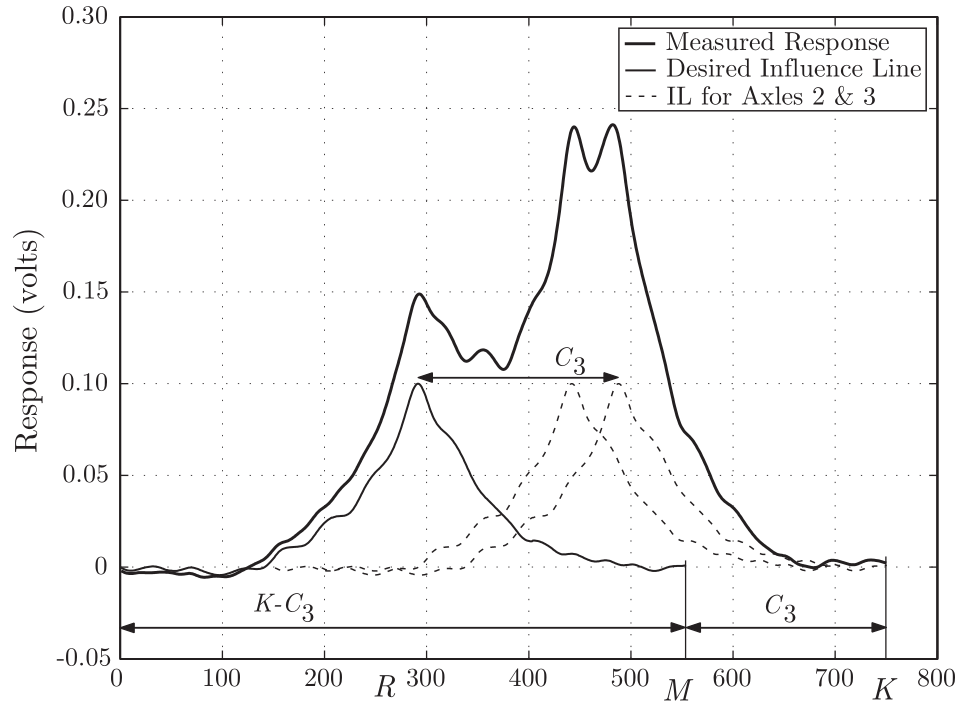
\includegraphics[width=\textwidth]{figures/strain_vs_influenceline}
	\caption{Axle peaks in strain signal}
	\label{fig:axle_peaks}
\end{figure}

The influence line is



(The noise level seem to vary according to sensor location.. Place in theory maybe!!)
